% \documentclass[a4paper,twocolumn,11pt,accepted=2017-05-09]{quantumarticle}
\documentclass[a4paper,twocolumn,10pt]{quantumarticle}
\pdfoutput=1
\usepackage[utf8]{inputenc}
\usepackage[english]{babel}
\usepackage[T1]{fontenc}
\usepackage{amsmath}
\usepackage{hyperref}

\usepackage{tikz}
\usepackage{lipsum}

\newtheorem{theorem}{Theorem}


\usepackage{tikz}
\usepackage{qcircuit}
%%%%%%%%%%%%%%%%%%

%\usepackage{IEEEtrantools}
\usepackage{multirow}

% ------------------------------------------------------------------------------
\newcommand{\rev}{\color{blue}}
\newcommand{\bae}{\color{purple}}
\newcommand{\ji}{\color{gray}}

\newcommand{\vx}{\Vec{x}}
\newcommand{\vy}{\Vec{y}}
\newcommand{\vo}{\Vec{0}}
\newcommand{\Va}{\Vec{a}}
\newcommand{\Vb}{\Vec{b}}
\newcommand{\power}[1]{^{\otimes #1}}
\newcommand{\lb}{\nonumber \\}


\newcommand{\R}{\mathbb{R}}
\newcommand{\N}{\mathbb{N}}
\newcommand{\C}{\mathbb{C}}
\newcommand{\Z}{\mathbb{Z}}
\newcommand{\Q}{\mathbb{Q}}
\newcommand{\I}{\mathbbm{1}}

\newcommand{\tr}{\text{tr}}
\newcommand{\ket}[1]{| #1 \rangle}
\newcommand{\bra}[1]{\langle #1|}
\newcommand{\ip}[2]{\langle #1|#2 \rangle}
\newcommand{\bracket}[3]{\langle #1|#2|#3 \rangle}
\newcommand{\sm}[1]{\left( \begin{smallmatrix} #1 \end{smallmatrix} \right)}

\newcommand{\be}{\begin{equation}}
\newcommand{\ee}{\end{equation}}
\newcommand{\bea}{\begin{eqnarray}}
\newcommand{\eea}{\end{eqnarray}}
\newcommand{\bes}{\begin{equation*}}
\newcommand{\ees}{\end{equation*}}
\newcommand{\beas}{\begin{eqnarray*}}
\newcommand{\eeas}{\end{eqnarray*}}

% ------------------------------------------------------------------------------

\newcommand{\x}{\mathrm{x}}
%\newcommand{\ket}[1]{|#1\rangle}
\newcommand{\ketbra}[1]{\ket{#1}\!\bra{#1}}
%\newcommand{\bra}[1]{\langle#1|}
\newcommand{\dyad}[1]{\ket{#1}\!\bra{#1}}

\newcommand{\ten}{\otimes}
\newcommand{\Id}{\mathds{1}}
\newcommand{\zero}{\mathbf{0}}
\newcommand{\KBDS}{C^{s}}
\newcommand{\KBDSs}{C}
%\newcommand{\KBDS}{C^{\mbox{\tiny U}}}
\newcommand{\KTwo}{C^{2\times2}}
\renewcommand{\H}{\mathcal{H}}
\def\A{\mathcal{A}}
\def\B{\mathcal{B}}

\def\x{\mathrm{x}}
\def\y{\mathrm{y}}

\def\W{\mathcal{W}}


\def\sig{\widetilde{\sigma}}
\def\F{\mathcal{F}}
\def\N{\mathcal{N}}
\def\P{\mathbbm{P}}
\def\tr{\mathrm{tr}}

\def\L{\mathcal{L}}
\def\Q{\mathcal{Q}}
\def\NL{\mathcal{NS}}

\DeclareMathOperator*{\Oplus}{\bigoplus}
\DeclareMathOperator*{\Otimes}{\bigotimes}
% \DeclareMathOperator*{\Oplus}{\scalerel*{\bigoplus}{\textstyle\sum}}
% ------------------------------------------------------------------------------






\begin{document}

\title{ Detecting Entanglement by State Preparation and Local Measurements}


\author{Jaemin Kim}
\email{woals6584@kaist.ac.kr}
\affiliation{School of Electrical Engineering, Korea Advanced Institute of Science and Technology (KAIST), 291 Daehak-ro, Yuseong-gu, Daejeon 34141, Republic of Korea }
\orcid{ }


\author{Anindita Bera}
\email{aninditatitli@gmail.com}
\affiliation{Department of Mathematics, Birla Institute of Technology Mesra, Jharkhand 835215, India}
\orcid{ }


\author{Dariusz Chru\'sci\'nski}
\email{darch@fizyka.umk.pl}
\affiliation{Institute of Physics, Faculty of Physics, Astronomy, and Informatics, Nicolaus Copernicus University, Grudziadzka 5, 87-100 Torun, Poland}
\orcid{ }

\author{Joonwoo Bae}
\email{joonwoo.bae@kaist.ac.kr}
\affiliation{School of Electrical Engineering, Korea Advanced Institute of Science and Technology (KAIST), 291 Daehak-ro, Yuseong-gu, Daejeon 34141, Republic of Korea }
\orcid{ }


\maketitle

\begin{abstract}
  Entanglement witnesses (EWs) are a collection of observables that can characterize separable states and, experimentally, estimating EWs can verify entangled states. In this work, we show that a fixed measurement setting on a multipartite entangled state, which we introduce as a \emph{network state} for the purpose, can estimate EWs. Namely, entangled states can be fully verified in a measurement-based manner, in which experimenters do not necessarily change measurement settings. We present a fixed measurement setting and network states for estimating decomposable EWs, equivalent to the partial transpose criteria. We also consider non-decomposable EWs that detect bound entangled states beyond the partial transpose criteria. The results can be extended to multipartite states such as graph states, a resource for measurement-based quantum computing, and readily applied to distributed settings such as quantum metrology or sensor networks where multipartite entangled states are resourceful.
\end{abstract}





\section{Introduction}


{Entangled states are a key resource in quantum information processing, in particular, to achieve quantum advantages in computation and communication tasks. A higher level of security in cryptographic protocols \cite{PhysRevLett.98.230501}, higher level of quantum certification \cite{Pironio_2009, PhysRevLett.110.060405, PhysRevLett.108.200401, Bowles:2018aa} and higher network channel capacities \cite{PhysRevA.95.052329, PhysRevLett.125.150502} can be achieved by exploiting entangled states. Efficient computation with quantum resources can be realized by local measurements and entangled states only, called measurement-based quantum computation (MBQC) \cite{PhysRevLett.86.5188, MeasurementBasedQuantumComputation, Briegel:2009aa}. }

{ Entanglement witnesses (EWs) \cite{TERHAL2000319, PhysRevA.62.052310} are versatile tools to detect entangled states both theoretically and experimentally. They correspond to observables that are non-negative for all separable states but negative for some entangled states \cite{HORODECKI19961, GUHNE20091, RevModPhys.81.865, Chru_ci_ski_2014, Friis:2019aa}. Hence, negative expectation values of EWs unambiguously conclude the presence of entangled states. In practice, multiple measurement settings may be necessary for estimating EWs. }

{ In this work, we show that a fixed measurement setting can detect entangled states, together with the preparation of a multipartite state, which we call a {\it network state}. To be precise, we present a framework for detecting entangled states such that a fixed measurement over a network state $N$ and a state $\rho$ can find if the state $\rho$ is entangled, where a network state $N$ is obtained from an EW. Thus, entangled states can be verified in a measurement-based (MB) manner. In fact, the framework is closely connected to the activation of entanglement in that it finds if a state $\rho$ is entangled if a joint state $N\otimes \rho$ is more entangled than a state $N$. }

We show how network states can be obtained from EWs. We present the construction of network states for decomposable EWs, which are equivalent to the partial transpose criteria, and also for non-decomposable EWs that detect bound entangled states beyond the partial transpose criteria, such as the Bell-diagonal EWs \cite{chruscinski2014class, PhysRevA.105.052401} from the Choi map \cite{Choi:1975aa} and its various generalizations \cite{PhysRevA.84.024302}, and the Breuer-Hall EW \cite{PhysRevLett.97.080501, Hall_2006}. The results are extended to multipartite systems: graph states \cite{PhysRevA.69.062311}, a resource for MBQC \cite{PhysRevLett.86.5188}, can be detected by network states and a fixed measurement.
{ 
We discuss the connection of our work to the entanglement activation \cite{PhysRevLett.96.150501} and the measurement-device-independent entanglement witnesses \cite{PhysRevLett.110.060405}.
}

The importance of our results is threefold. Firstly, similarly to MBQC, one can circumvent the control of multiple measurement settings when estimating observables. Precise controls on and the preparation of general measurements identify additional difficulties for realizing EWs in general. Our results show that the preparation of quantum states and a fixed measurement can be an experimentally feasible alternative. Secondly, it is of fundamental interest to find that entangled states with a fixed measurement are a resource that can be replaced with observables. Note that MBQC signifies that entangled states and local measurements can be an alternative to realize quantum state transformation. Finally, the framework for estimating EWs in an MB manner finds various usefulness of distributed settings such as distributed quantum metrology over networks, e.g., \cite{Chabuda:2020aa, Zhang_2021,Len:2022aa, PhysRevLett.121.043604}: estimation of joint observables enables distributed quantum information processing, e.g., \cite{PhysRevA.85.062326, Friis_2017, PhysRevLett.120.080501}.

\section{Entanglement detection}
 
Let us begin by describing an experimental scenario of verifying entangled states, where the scenario is common in various experimental settings. We consider two quantum systems $A$ and $B$ on a Hilbert space $\H\otimes \H$. Interestingly, observables exist, denoted by $W=W^{\dagger}$, such that, for all separable states $\sigma_{\mathrm{sep}}$, 
\bea
\tr[W\sigma_{\mathrm{sep}}] \geq 0~~\mathrm{and }~~ \tr[W\rho_{\mathrm{ent}}] <0\nonumber
\eea
for some entangled states $\rho_{\mathrm{ent}}$ \cite{TERHAL2000319, PhysRevA.62.052310}. All entangled states can be verified by estimating some observables, which are called entanglement witnesses (EWs). In experiment, EWs can be estimated by altering measurement settings in general: negative expectation values unambiguously conclude entangled states \cite{GUHNE20091}. They can be also used to verify other properties, other than entanglement, such as a fidelity in the state preparation \cite{PhysRevA.76.030305, Haffner:2005aa}.

%Note that the structure of EWs remains } 


%One of the intriguing properties of entangled states is the irreversibility in manipulations of entanglement. Entangled states from which no entanglement can be extracted, though entanglement is needed for their preparation, are identified as {\it undistillable} or {\it bound} entangled states \cite{PhysRevA.61.062313, PhysRevLett.86.2681}. Multipartite quantum states that remain positive after partial transpose (PPT) turn out to be undistillable. Remarkably, PPT entangled states can be used to activate other entangled states \cite{horodecki1999bound}.

%Then, non-PPT entangled states can be characterized by decomposable EWs that have a general form as follows,
%\bea
%W = P+Q^{\Gamma},~~\mathrm{for}~~P,~Q\geq 0\nonumber.
%\eea
%Here $\Gamma$ denotes the partial transpose. Then, non-decomposable EWs, which cannot be in the form above, can detect PPT entangled states. 

%\cite{PhysRevA.61.062313, PhysRevLett.86.2681}.

%In general, it is highly non-trivial to construct non-decomposable EWs, which are the main object in the mathematically challenging problem of classifying positive linear maps of Operator Algebras \cite{Stormer:1963aa}, see also Refs. \cite{bera2022generalizing, bera2022class,mirror}.

{\section{Measurement-Based Estimation}

Let us show that observables can be generally estimated in a measurement-based manner. We here focus on EWs, observables of particular interest for detecting entangled states, and provide the scheme for estimating of single observables in Appendix. We devise multipartite quantum states, {\it called network states}, for estimating observables. 

\subsection{Example }
\label{subsec:ex}
Let us begin with an illuminating example of an MB estimation of an EW. Throughout, Bell states are denoted by $|\phi^{\pm}\rangle = (|00\rangle \pm |11\rangle)/\sqrt{2}$ and $|\psi^{\pm}\rangle = (|01\rangle \pm |10\rangle)/\sqrt{2}$. We consider an EW in the following,
\bea
%W = \frac{1}{2} \mathbbm{1} - |\psi^{-} \rangle \langle \psi^{-} |, \nonumber
W = \frac{1}{4} (\mathbbm{1} + X\otimes X + Y\otimes Y + Z\otimes Z) \label{eq:ewex}
\eea
where $X,Y$ and $Z$ are Pauli matrices. Eq. (\ref{eq:ewex}) shows that an EW can be estimated by various measurement settings. Note that a Bell state $|\psi^{-}\rangle$ is detected by an EW above. 
 
 
%\subsection{Two-qubit network states}

The MB framework for estimating an observable in Eq. (\ref{eq:ewex}) can be achieved by a four-partite state, called a {\it network state}, constructed as follows, 
\bea
N_{23} &=& \frac{1}{4} |\psi^-\rangle_{A_2B_2} \langle \psi^-| \otimes |\phi^+\rangle_{A_3B_3} \langle \phi^+| + \nonumber \\
&&\frac{1}{12} (\mathbbm{1} - |\psi^-\rangle_{A_2B_2} \langle \psi^-|) \otimes (\mathbbm{1} - |\phi^+\rangle_{A_3B_3} \langle \phi^+|),~~~~ ~\label{eq:wr}
\eea

on sites $A_2A_3B_2B_3$, see Fig. \ref{fig:fig1}. We then place a state of interest at $A_1B_1$, denoted by $\rho_{1}:=\rho^{( A_1B_1)}$, which we want to learn if it is entangled. We have
\bea
\tr[\rho W ] =  16~ \tr  [\rho_1\otimes N_{23} (\frac{1}{2}\mathbbm{1} - | \phi^+\rangle_{A_3B_3} \langle \phi^+|) \otimes P^{(12)}],~~
\label{eq:ewr}
\eea
where $P^{(12 )} = |\phi^{+}\rangle_{A_1A_2}\langle \phi^+| \otimes |\phi^{+}\rangle_{B_1B_2}\langle \phi^+|$. Eq. (\ref{eq:ewr}) can be simplified by a singlet fraction as follows,
\bea
_{A_3 B_3}  \langle \phi^{+}| \tr_{12}[ \rho_1 \otimes N_{23} ~P^{(12)} ]  |\phi^{+}\rangle_{A_3 B_3}   = \frac{1}{8} - \frac{1}{4}\tr[\rho W].~~
\label{eq:expew}
\eea
The left-hand-side can be obtained by preparing a network state followed by a fixed measurement. A state $\rho_1$ is entangled if the right-hand-side is greater than $1/8$ since $\tr[\sigma_{\mathrm{sep}}W ]\geq 0 $ for all separable states $\sigma_{\mathrm{sep}}$. Once a Bell measurement reports an outcome $P^{(12)} $, a singlet fraction is estimated from the probability of having outcome $|\phi^{+}\rangle$ on $A_3B_3$. Thus, it is shown that an EW can be estimated in a fully MB manner. 

%In fact, an entangled state $\rho$ is detected if the probability, i.e., the left-hand-side in Eq. (\ref{eq:expew}), is greater than $1/8$, since $\tr[\sigma_{\mathrm{sep}}W ]\geq 0 $ for all separable states $\sigma_{\mathrm{sep}}$.


Experimental resources to realize the MB framework, i.e., the left-hand side in Eq. (\ref{eq:expew}), are as follows. A network state is required, see Eq. (\ref{eq:ewex}), which is entangled and bi-separable. The detection scheme needs a measurement in the basis $|\phi^+\rangle$, which is equivalent to the capability of realizing a controlled-NOT gate, a Hadamard gate, and a fixed-measurement in the $z$-direction; see also Fig. \ref{fig:fig1}. All these are compatible with the resources to realize MBQC. In addition, it is worth mentioning that a network state in Eq. (\ref{eq:wr}) is a variation of a Smolin state, a four-partite bound entangled state \cite{PhysRevA.63.032306}, which has been repeatedly realized in experiment \cite{ Amselem:2009aa, PhysRevLett.105.130501, PhysRevLett.109.040501}. It should be pointed out that a realization of the presented MB framework is readily available in an experiment. 



\begin{figure}[t]
\centering
% \includegraphics[width=9.0cm ]{figure1}
\resizebox{0.9\linewidth}{!}{
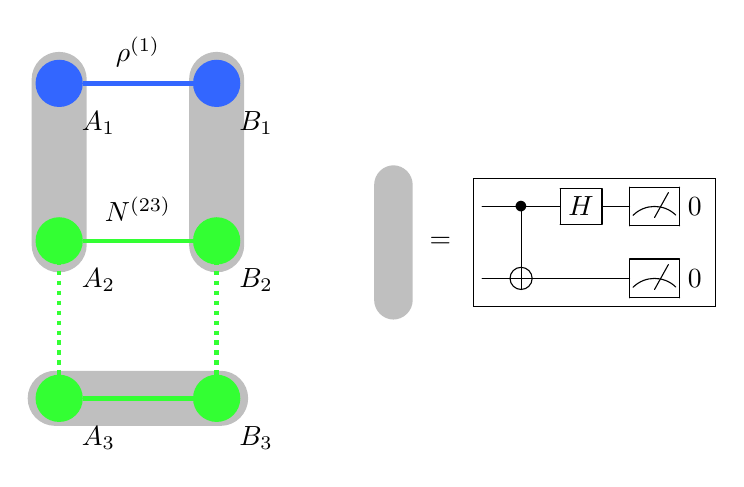
\begin{tikzpicture}[scale=2]
    % Define custom colors
    \definecolor{customBlue}{rgb}{0.2, 0.4, 1}
    \definecolor{customGreen}{rgb}{0.2, 1, 0.2}

    % Round-edged rectangles and dotted lines for both rows
\fill[lightgray, rounded corners=0.35cm] (-0.175,1.2) rectangle (0.175,-0.2);
\fill[lightgray, rounded corners=0.35cm] (-1-0.175,1.2) rectangle (-1+0.175,-0.2);
\fill[lightgray, rounded corners=0.35cm] (-0.5-0.7,-0.825) rectangle (-0.5+0.7,-1.175);
\draw[customGreen, ultra thick, dotted] (0,0) -- (0,-1);
\draw[customGreen, ultra thick, dotted] (-1,0) -- (-1,-1);

% Green ultra thick lines between A2-B2 and A3-B3
\draw[customGreen, ultra thick] (0.15,0) -- (-1+0.15,0);
\draw[customGreen, ultra thick] (0.15,-1) -- (-1+0.15,-1);

% Blue ultra thick line between A1 and B1
\draw[customBlue, ultra thick] (0.15,1) -- (-1+0.15,1);

    % First row of disks
    \fill[customBlue] (0,1) circle (0.15);
    \fill[customGreen] (0,0) circle (0.15);
    \fill[customGreen] (0,-1) circle (0.15);

    % Second row of disks
    \fill[customBlue] (-1,1) circle (0.15);
    \fill[customGreen] (-1,0) circle (0.15);
    \fill[customGreen] (-1,-1) circle (0.15);

    % Captions
    \node at (-0.5,1.2) {$\rho^{(1)}$};
    \node at (-0.5,0.2) {$N^{(23)}$};

% Labels
\node at (-1+0.25,0.75) {$A_1$};
\node at (-1+0.25,-0.25) {$A_2$};
\node at (-1+0.25,-1.25) {$A_3$};
\node at (+0.25,0.75) {$B_1$};
\node at (+0.25,-0.25) {$B_2$};
\node at (+0.25,-1.25) {$B_3$};

    \begin{scope}[xshift=1cm, yshift=-0.5cm, scale=0.7] % Adjust yshift for spacing between figures
        \fill[lightgray, rounded corners=0.25cm] (0,0) rectangle (0.35,1.4);

        \node at (0.6,0.7) {$=$};

        % Quantum Circuit inside a TikZ node
        \node[draw, inner sep=3pt] at (2,0.7) {
            \Qcircuit @C=1em @R=1.2em {
            % Qubit setup
            \lstick{} & \ctrl{1} & \gate{H} & \meter & \rstick{\hspace{-1.2em} 0} \\
            \lstick{} & \targ    & \qw      & \meter & \rstick{\hspace{-1.2em} 0} \\
            }
        };
    \end{scope}
\end{tikzpicture}
}
\caption{ A four-partite network state $N_{23}$ is prepared on $A_2A_3B_2B_3$ to detect an entangled state on $A_1B_1$. Bi-interactions and measurements in the computational basis can construct EWs, see also Eq. (\ref{eq:expew}) in the text. Gray boxes denote a measurement in the basis $|\phi^{+}\rangle$, which is equivalent to a measurement in the computational basis after applying of a controlled-NOT gate followed by a Hadamard gate. }
\label{fig:fig1}
\end{figure}



\subsection{ EWs via entanglement activation}

To show a general construction of network states for arbitrary EWs for high-dimensional quantum systems, we want to clarify their relations to activation of entanglement \cite{PhysRevLett.96.150501}: all EWs can be expressed in the following form, }
\bea
W_{A_2 B_2 } = \tr_{A_3B_3} \big[N (\eta \mathbbm{I} - |\phi_{d}^+ \rangle_{A_3B_3} \langle \phi_{d}^+ |)\big], \label{eq:ewm}
\eea
for some network state $N := N^{(A_2 B_2 A_3 B_3)}$ and a parameter $\eta \in [1/d,1 )$, where $|\phi_{d}^+\rangle = \sum_{j=0}^{d-1}|jj\rangle /\sqrt{d}$. It is worth mentioning an EW above shares similarity with Eq. (\ref{eq:ewr}) Note that the parameter $\eta$ satisfies the condition, $\eta\geq E_d [N]$ where $E_d$ is called a maximal singlet fraction,
\bea
E_d[N] &=& \sup_{\F}~ \langle \phi_{d}^+| \F[ N ] |\phi_{d}^+\rangle ~\mathrm{for~a~local ~filtering~}\F   \nonumber \\
&& \F[N] = \frac{ K_{A}\otimes K_B N K_{A}^{\dagger}\otimes K_{B}^{\dagger} }{ \tr[  K_{A}^{\dagger}K_{A} \otimes K_{B}^{\dagger}K_{B} N ]},\label{eq:fil}
\eea
where $K_A: \H_{A_1A_2}\rightarrow \mathbbm{C}^d $ and $K_B: \H_{B_1B_2}\rightarrow \mathbbm{C}^d $. It is worth mentioning that EWs in Eq. (\ref{eq:ewm}) identify entangled states that activate a network state in the sense that
\bea
E_d[ \sigma\otimes N]>\eta, ~\mathrm{whereas}~ {E_d [N]\leq \eta}.\label{eq:ac}
\eea
In fact, all entangled states can be used to activate some other state: in Eq. (\ref{eq:ac}) a state $\sigma$ is entangled if and only if it can activate some other entangled state $N$.



{ 
\subsection{ Detection protocol from  entanglement activation}

We exploit the scenario of activating entanglement as a framework for detecting entangled states. Namely, a state $\rho$ is entangled if it can be used to activate a state $N$. To this end, we consider a local filtering operation $\Phi$ as follows,
\begin{align}
\Phi (\rho \otimes N) = \tr_{A_1 B_1 A_2 B_2}[ P^{(12)} \rho^{(A_1 B_1)} \otimes N^{(A_2 B_2 A_3 B_3)}]. \nonumber
\end{align}
where $P^{(12)}$ the projection onto maximally entangled states as follows,
\bea
P^{(12 )} = |\phi_{d}^{+}\rangle_{A_1A_2}\langle \phi_{d}^+| \otimes |\phi_{d}^{+}\rangle_{B_1B_2}\langle \phi_{d}^+| \label{eq:projd} 
\eea
and $|\phi_{d}^+\rangle = \sum_{i=1}^d|ii\rangle/\sqrt{d}$. The singlet fraction after the filtering operation is given by,
\begin{align}
F_{\Phi}(\rho \otimes N) = \frac{ \bracket{\phi_d^+}{\Phi(\rho \otimes N)}{\phi_d^+} }{\tr[\Phi(\rho \otimes N)]}.\nonumber
\end{align}
With the specific local operation, the singlet fraction of a network state $N$ can be computed as, 
\begin{align}
\widetilde E_d(N) = \sup_{\sigma \in \mathrm{SEP}} F_{\Phi}(\sigma \otimes N),
\end{align}
where $\mathrm{SEP}$ denotes the set of separable states. It is clear that $\widetilde E_d(N) \le E_d(N)$ since a specific local operation is considered. Note also that for $\eta \in [\frac{1}{d},1)$, there exists a state $N$ such that $E_d(N) = \widetilde E_d(N) = \eta$ \cite{PhysRevLett.96.150501}. It holds that a state $\rho$ is entangled if we have $F_{\Phi}(\rho \otimes N) > \eta $ for $N$ such that $\widetilde E_d(N) \leq \eta$. 
}




\subsection{ General construction of network states }
\label{sec:gc}

Let us then present a construction of a network state for a given EW, see also Eq. (\ref{eq:ewm}). Suppose that an EW on $d\otimes d$ is decomposed as follows,
\bea
W = \sum_{j} a_j W(j)^T ~\mathrm{with}~ W(j) \geq 0 ~\mathrm{and}~ a_j \in \mathbbm{R}, \label{eq:eeww}
\eea
so that one can choose normalized non-negative operators $\{ \Pi(i) \geq 0\}$ and real constants $\{ c_j\}$ such that,
\bea
N_{23} &=&\sum_{j} c_j  W(j)_{A_2B_2} \otimes  \Pi(j)_{A_3B_3}, ~\mathrm{and}  \label{eq:ns} \\
W_2 & =& ~ k \, \tr_{3} [N_{23}^{T_2}  ( \eta \mathbbm{1} - |\phi_{d}^+ \rangle_{A_3B_3} \langle \phi_{d}^+ |  )  ], \label{eq:ewn}
\eea
for some $\eta\geq 1/d$ and $k>0$, where $W_2$ reproduces a given EW in Eq. (\ref{eq:eeww}) on sites $A_2 B_2$. One can find $\{a_j\}$ and $\{c_j \}$ are related as follow,
\bea
a_j = k \, c_j (\eta - \bracket{\phi_{d}^+}{\Pi(j)}{\phi_{d}^+}).\nonumber
\eea
Then, for a state $\rho_1 = \rho^{(A_1B_1)}$ it holds that
\bea
\tr[\rho W] %&=& d^2 ~ \tr[\rho_1 \otimes W_{2}^T P^{(12)}  ]  \nonumber\\
&\propto& \tr[\rho_1 \otimes N_{23} ~ P^{(12)} \otimes ( \eta \mathbbm{1} - |\phi_{d}^+ \rangle_{A_3B_3} \langle \phi_d^+ |  ) ]. ~~~~~ \label{eq:m}
\eea
For an entangled state $\rho$ detected by $W$, i.e., $\tr[\rho W]<0$, Eq. (\ref{eq:m}) shows that
\bea
\eta &<&  _{A_3B_3}\langle \phi_{d}^+| \Lambda^{(1\rightarrow 3)} [\rho_1]|\phi_{d}^+\rangle_{A_3B_3} \nonumber \\
&&\mathrm{where}~ \Lambda^{( 1\rightarrow 3)} [\rho_1]= \frac{ \tr_{12}[\rho_{1}\otimes N_{23} P^{(12)}] }{ \tr[\rho_1\otimes N_{23} P^{(12)}]  }. ~~\label{eq:v}
\eea
Note that the construction above applies to all EWs in general.\\

{
{\it Example.} A straightforward and facile construction of a network state from an EW is as follows. For an EW, we find a decoposition,
\bea
 W = a_+ W_+^T - a_- W_-^T\nonumber
 \eea
with coefficients $a_{\pm} > 0$ and quantum states $W_{\pm}$ (i.e., $W_{\pm} \ge 0$ and $\tr[W_{\pm}]=1$). We choose $\eta = 1/d$ and find a network state as follows,
\begin{align}
N_{23} &=c_+ W_+ \otimes \frac{\I-\dyad{\phi^+_d}}{d^2-1} +  c_- W_- \otimes \dyad{\phi^+_d}.\nonumber
\end{align}
where
\bea
c_+ = \frac{(d-1)a_+}{(d-1)a_+ + a_-} ~~\mathrm{and} ~~c_-= \frac{a_-}{(d-1)a_+ + a_-}. \nonumber
\eea 
We have presented a straightforward one by exploiting a spectral decomposition of an EW. We also stress that a network state is not unique for an EW. \\
}

A quantum teleportation protocol may rephrase Eq. (\ref{eq:v}) as follows. Once a measurement $P^{(12)}$ is successful, a state $\rho$ prepared at $A_1B_1$ is teleported at $A_3B_3$ via a network state $N_{23}$. Note that the map in Eq. (\ref{eq:v}) is a probabilistic operation assisted by entanglement \cite{PhysRevA.64.012317}; to be precise, successful Bell measurements define a channel for a state $\rho_1$ \cite{Jamiokowski:1972aa, Choi:1975aa}. Finally, a singlet fraction is estimated and compared with $\eta$, see Eq. (\ref{eq:v}), to verify entanglement. We have shown that, given an EW, one can always construct a network state for the estimation as above. 

As mentioned, experimental resources for the realization contain preparing a network state and Bell measurements that require bi-interactions and a fixed local measurement setting; see also Fig. \ref{fig:fig1}. In Appendix, we reproduce a network state in Eq. (\ref{eq:wr}) by applying the general construction above.

{
\subsection{ Noisy local projections on $A_1A_2$ and $B_1B_2$: semi measurement-device-independent entanglement witnesses } 
\label{semi MDI}

The framework of detecting entanglement relies on projections to maximally entangled states, see Eq. (\ref{eq:projd}). It bears some similarity with the measurement-device-independent (MDI) scenario \cite{PhysRevLett.108.200401,PhysRevLett.110.060405}, which applies when one wants to relax the assumption to trust measurement devices. Then, an MDI scenario trusts on state preparations and relaxes the assumptions on joint measurements. 

Similarly, we here show that projections on  $A_1A_2$ and $B_1B_2$, joint measurements performed locally, can be relaxed for the verification of entangled states. To this end, we show that untrusted joint measurements on $A_1A_2$ and $B_1B_2$ can unambiguously conclude entangled states. Let us consider a separable state $\sigma = \sum_k p_k \tau_k \otimes \xi_k$ and a threshold  $\eta$. Let $Q^{(A_1 A_2)}$ and $R^{(B_1B_2)}$ denote unknown positive-operator-valued-measure elements that may describe detection events of untrusted measurement devices. It suffices to show that $\sigma$ cannot increase the singlet fraction of $N$ larger than the threshold $\eta$. This means, 
\bea
\tr[(Q^{(A_1 A_2)} \otimes R^{(B_1 B_2)} \sigma_1 \otimes W_{2}^T]  \geq 0 \nonumber
\eea
for all $Q$ and $R$, see also $W_{2}^T$ in Eq. (\ref{eq:ewn}). We then have: 
\bea
&& \sum_k p_k \tr[(Q^{(A_1 A_2)} \otimes R^{(B_1 B_2)}) (\tau_k^{(A_1)} \otimes \xi_k^{(B_1)}) W_{2}^T ] \nonumber \\
%&=& \sum_k p_k \tr[(\widetilde{Q}^{(A_2)} \otimes \widetilde{R}^{(B_2)}) N_{23} (\eta \I - \dyad{\phi^+_d})_3] \nonumber \\
%&\propto \sum_k p_k \tr[(\widetilde{Q} \otimes \widetilde{R})_2 W^T_2] \nonumber\\
&\propto& \sum_k p_k \tr[(\widetilde{Q}^T \otimes \widetilde{R}^T) W] \ge 0 \nonumber 
\eea
since 
\begin{align*}
\widetilde{Q}^{(A_2)} &= \tr_{A_1}[Q^{(A_1 A_2)} (\sigma_k^{(A_1)} \otimes \I^{(A_2)})] \ge 0, \\
\widetilde{R}^{(B_2)} &= \tr_{B_1}[R^{(B_1 B_2)} (\xi_k^{(B_1)} \otimes \I^{(B_2)})] \ge 0\nonumber
\end{align*}
and an EW is non-negative for all separable states. Hence, we have shown that joint measurements on $A_1A_2$ and $B_1B_2$ with untrusted measurements can also unambiguously conclude entangled states. 
}

\section{Examples}


Let us apply the general construction of network states and present network states for EWs known so far, such as decomposable and non-decomposable instances, the latter of which are highly non-trivial in Quantum Information Theory. Identifying all EWs is equivalent to characterizing the set of separable states, which is a challenging mathematical problem \cite{Stormer:1963aa}; the computational complexity also belongs to NP-Hard \cite{10.1145/780542.780545}. The construction of network states applies to all EWs. In what follows, we apply the general construction of network states to non-trivial EWs.

To this end, let $P_{st}$ denote a projection onto a Bell state, for $s,t = 0,\ldots, d-1$, in a dimension $d$,
\bea
P_{st} = |\phi_{st}\rangle \langle \phi_{st}| ~\mathrm{where}~|\phi_{st} \rangle = \frac{1}{\sqrt{d}} \sum_{j = 0}^{d-1} \omega^{t j } \ket{j } \ket{j + s}, ~~ \label{eq:1}
\eea
where $\omega = e^{2\pi i/d}$.
Projectors onto symmetric and anti-symmetric subspaces are denoted by $S_d$ and $A_d$, respectively,
\bea
S_d = \frac{\mathbbm{1+F} }{2}~~\mathrm{and} ~~A_d = \frac{\mathbbm{1 - F} }{2},
\eea
where $\mathbbm{F} = d P_{00}^{\Gamma}$ is a flip operator and $\Gamma$ denotes the partial transpose \cite{PhysRevA.61.062313}. Note that $\tr[A_d]=d(d-1)/2$ and $\tr[S_d] = d(d+1)/2$. Interestingly, high-dimensional Bell states and projections onto symmetric and anti-symmetric subspaces suffice to construct network states for known non-decomposable maps.



\subsection{ Decomposable EWs: the partial transposition }

Firstly, we consider a decomposable EW $W = Q^\Gamma$ for $Q\geq 0$ and $\tr[Q]=1$, for which a network state can be constructed as follows. We write by $\lambda:=\max_{i}|\lambda_i|$ where $\{\lambda_i\} $ are eigenvalues of an EW $W$ and a network state is obtained as,
\bea
N_{23}&=& c_1\left( \frac{\lambda\mathbbm{1} - Q^\Gamma }{\lambda d^2 - 1 }\right)^{(2)} \otimes P_{00}^{(3)} \nonumber\\
&&+ c_2 \left( \frac{ \lambda \mathbbm{1} +  Q^{\Gamma} }{\lambda d^2 + 1}\right)^{(2)} \otimes \left( \frac{\mathbbm{1} - P_{00}}{d^2 - 1}\right)^{(3)}, \label{eq:nsd}
\eea
where superscript $(j)$ stands for systems $A_jB_j$ and
\bea
c_1 = \frac{d^2 \lambda - 1}{d^3 \lambda  + d -2} ~~\mathrm{and}~ ~ c_2 =\frac{(d-1)(d^2 \lambda +1)}{d^3 \lambda  +d-2}. \nonumber
\eea
In the other way around, from a network state $N_{23}$ in Eq. (\ref{eq:nsd}) one can reproduce a decomposable EW, see Eq. (\ref{eq:ewm})
\bea
\tr_3[ N_{23 } (\frac{1}{d} \mathbbm{1} - |\phi_{00}\rangle_{A_3B_3}\langle \phi_{00}|)] = \frac{2(d-1)}{d(d^3 \lambda + d -2)} Q^\Gamma \propto Q^\Gamma.\nonumber
% \\ \tr_3[ N_{23}^{(\mathrm{BH})}~ (\frac{1}{d} \mathbbm{1} - |\phi_{00}\rangle_{A_3B_3}\langle \phi_{00}|)] = \frac{2(d-1)}{d(d^3 \lambda + d -2)} Q^\Gamma \propto Q^\Gamma.\nonumber
\eea
Hence, the partial transpose criteria \cite{PhysRevLett.77.1413} can be generally realized by preparing a network state with a fixed measurement.

As an instance, a network state for the decomposable and optimal EW $W = P_{00}^{\Gamma}$ can be found as
\bea
\frac{1}{d+2} \left( \frac{A_d}{\tr A_d} \right)^{(2)} \otimes P_{00}^{(3)}  +  \frac{d+1}{d+2} \left( \frac{S_d}{\tr S_d} \right)^{(2)} \otimes \left( \frac{\mathbbm{1}-P_{00}}{d^2-1} \right)^{(3)}. \nonumber
\eea
The network state above is known as a symmetric state being $UUVV^*$-invariant, and has been used to activate entanglement distillation with an infinitesimal amount of bound entanglement \cite{PhysRevLett.88.247901}.

\subsection{ Non-decomposable EWs }

Secondly, to construct network states for non-decomposable EWs, we introduce paired Bell-diagonal (PBD) states as follows,
\bea
N_{23}^{(\mathrm{PBD})}(\Vec{\lambda}) = \sum_{s=0}^{d-1} \lambda_s ~\frac{1}{d} \sum_{t=0}^{d-1}  P_{st}^{(2)} \otimes P_{st}^{(3)}, \label{eq:PBD}
\eea
where $\Vec{\lambda}=(\lambda_0, \ldots, \lambda_{d-1})$ and $\sum_{s=0}^{d-1} \lambda_s = 1$.


\subsubsection*{ Bell-diagonal EWs}

A network state in Eq. (\ref{eq:PBD}) can be used to estimate expectation values of Bell-diagonal EWs \cite{chruscinski2014class},
 \bea
W[\Vec{\lambda}] = \sum_{s=0}^{d-1} \lambda_s \Pi_s - P_{00},~~\mathrm{where}~~ \Pi_s = \sum_{t=0}^{d-1} P_{st}.
\label{eq:Wa}
\eea
Note that the Choi map and its generalizations are well-known instances. Then, PBD network states construct Bell-diagonal EWs as follows,
\bea
\frac{\lambda_0}{d} W_2^T [\Vec{\lambda}] &=& \tr_3[ N_{23}^{(\mathrm{PBD})}(\Vec{\lambda}) (\lambda_0 \mathbbm{1} - |\phi_{00}\rangle_{A_3B_3}\langle \phi_{00}|)]. \nonumber
\eea
Hence, it is shown that all entangled states characterized by Bell-diagonal EWs can be detected by a fixed measurement and state preparation.

\subsubsection*{Choi EWs}

Instances of Bell-diagonal EWs for $d=3$ contain the Choi map \cite{Choi:1975aa} and its generalizations \cite{PhysRevA.84.024302, doi:10.1142/S1230161213500066}, that detect PPT entangled states. As it is shown in Eq. (\ref{eq:v}), once a filtering operation with a PBD network state in Eq. (\ref{eq:PBD}) is successful, entangled states are concluded by finding a singlet fraction. For the Choi map, entangled states are detected if the singlet fraction is larger than $2/3$. The proof is provided in Appendix.

\subsubsection*{Multipartite bound entangled states as a network state}

We also observe that a PBD state for $d=2$ with $\vec{\lambda} = (1/2,1/2)$ corresponds to a Smolin state \cite{PhysRevA.63.032306},
\bea
\rho_S = \frac{1}{4}\sum_{s,t=0,1 } P_{st}^{(A_2B_2)} \otimes P_{st}^{(A_3B_3)}. \nonumber
\eea
The state is invariant under permutations of $A_2A_3B_2B_3$ and remains PPT in any bipartite splitting: it is called a four-partite unlockable and undistillable entangled state. A Smolin state can be used to activate distillation of entanglement.

A Smolin state can be generalized to higher dimensions, with $\vec{\lambda} = (1/d,\ldots,1/d)$,
\bea
N_{23} (\Vec{\lambda}) = \frac{1}{d^2} \sum_{s=0}^{d-1} \sum_{t=0}^{d-1}  P_{st}^{(A_2 B_2)} \otimes P_{st}^{(A_3B_3)}. \nonumber
\eea
However, a Smolin state in a higher dimension $d>2$ no longer remains PPT in the bipartite splitting $A_2A_3:B_2B_3$. The network state then realizes an EW,
\bea
W = \frac{1}{d}\sum_{s=0}^{d-1}  \Pi_s - P_{00} = \frac{1}{d} \mathbbm{1} - P_{00} \label{reductionEW}
\eea
which is decomposable. It is also an EW that is derived from a reduction map \cite{PhysRevA.59.4206}. Note that a Smolin state corresponds to a network state that realizes a reduction EW for $d=2$.

\subsubsection*{ EWs from the Breuer-Hall map}


The Breuer-Hall (BH) map shown in Refs. \cite{PhysRevLett.97.080501, Hall_2006} derives highly non-trivial non-decomposable EWs,
\bea
\Lambda_{\textrm{BH}}(\rho) = \frac{1}{d-2} ( \tr(\rho) \mathbbm{1} - \rho - U \rho^T U^\dagger) \label{eq:BH map}
\eea
where $U$ is a skew-symmetric unitary operator satisfying $UU^\dagger = \mathbbm{1}$ and $U^T = -U$.
Then the BH EW is obtained as follows,
\bea
W_{\mathrm{BH}} = \frac{1}{d-2} ( \frac{1}{d}\mathbbm{1} - P_{00} - \frac{1}{d}\mathbbm{F}'), \label{eq:BH EW}
\eea
where $\mathbbm{F}' \equiv (\mathbbm{1} \otimes U) \mathbbm{F} (\mathbbm{1} \otimes U^\dagger)$. Note that the BH EW is optimal.

A network state for the BH EW is obtained as follows,
\bea
N_{23}^{(\textrm{BH})}  %& = & c_0 N^{(23)}_{\textrm{PBD}} + (1-c_0) N^{(23)}_{\textrm{skew}}, \label{eq:bhn} \\
& = & c_0 \frac{1}{d^2} \sum_{s=0}^{d-1} \sum_{t=0}^{d-1} P_{st}^{(2)}  \otimes P_{st}^{(3)} \nonumber \\
&& + c_1 \left( \frac{\mathbbm{1} + \mathbbm{F}' }{d^2+d} \right)^{(2)} \otimes P_{00}^{(3)}   \nonumber \\
&& + c_2 \left( \frac{\mathbbm{1} - \mathbbm{F}' }{d^2-d} \right)^{(2)} \otimes \left( \frac{\mathbbm{1} - P_{00}}{d^2-1} \right)^{(3)}, \label{eq:nbhh}
\eea
where
\bea
c_0 = \frac{2d^2-2d}{3d^2 -3d +2},~\mathrm{and}~ c_1= \frac{d+1}{3d^2-3d+2}, \nonumber
\eea
and $c_2 = 1-c_0-c_1$. One can find that, from Eq. (\ref{eq:ewn})
\bea
W_{\mathrm{BH}}^T ~~\propto~~ \tr_3[ N_{23}^{(\mathrm{BH})}~ (\frac{1}{d} \mathbbm{1} - |\phi_{00}\rangle_{A_3B_3}\langle \phi_{00}|)]. \label{eq:bh}
\eea
Once a filtering operation in Eq. (\ref{eq:v}) is successful, entangled states are detected if a singlet fraction of a resulting state on $A_3B_3$ is larger than $1/d$.


\begin{figure}[t]
\centering
% \includegraphics[width=9.2cm ]{figure2}
\resizebox{0.9\linewidth}{!}{
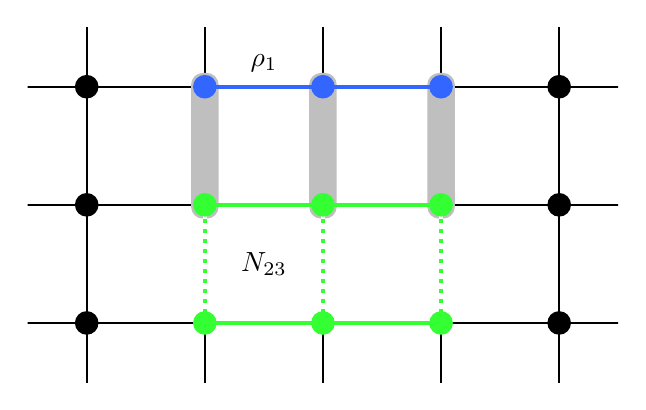
\begin{tikzpicture}[scale=0.5]
    % Define custom colors
\definecolor{customBlue}{rgb}{0.2, 0.4, 1}
\definecolor{customGreen}{rgb}{0.2, 1, 0.2}
\begin{scope}
\clip (-4.5,-1.5) rectangle (10.5,7.5);
\begin{scope}
    \foreach \x in {-6,-3,...,12} {
        \draw[thick, black] (\x,-3) -- (\x,9);
    }
    \foreach \y in {-3,0,...,9} {
        \draw[thick,black] (-6,\y) -- (12,\y);
    }
\end{scope}

    \fill[lightgray, rounded corners=0.15cm] (0-0.35,3+0-0.35) rectangle (0+0.35,6+0+0.35);
    \fill[lightgray, rounded corners=0.15cm] (3-0.35,3+0-0.35) rectangle (3+0.35,6+0+0.35);
    \fill[lightgray, rounded corners=0.15cm] (6-0.35,3+0-0.35) rectangle (6+0.35,6+0+0.35);

    \draw[customGreen, ultra thick] (0,0) -- (3,0) -- (6,0);  
    \draw[customGreen, ultra thick] (0,3) -- (3,3) -- (6,3);
    \draw[customBlue, ultra thick] (0,6) -- (3,6) -- (6,6);
    \draw[white, ultra thick] (0,0) -- (0,3);
    \draw[white, ultra thick] (3,0) -- (3,3);
    \draw[white, ultra thick] (6,0) -- (6,3);
    \draw[customGreen, ultra thick, dotted] (0,0) -- (0,3);
    \draw[customGreen, ultra thick, dotted] (3,0) -- (3,3);
    \draw[customGreen, ultra thick, dotted] (6,0) -- (6,3);


    \fill[black] (-3,0) circle (0.3);
    \fill[black] (-3,3) circle (0.3);
    \fill[black] (-3,6) circle (0.3);

    \fill[black] (9,0) circle (0.3);
    \fill[black] (9,3) circle (0.3);
    \fill[black] (9,6) circle (0.3);


    \fill[customGreen] (0,0) circle (0.3);
    \fill[customGreen] (3,0) circle (0.3);
    \fill[customGreen] (6,0) circle (0.3);

    \fill[customGreen] (0,3) circle (0.3);
    \fill[customGreen] (3,3) circle (0.3);
    \fill[customGreen] (6,3) circle (0.3);

    \fill[customBlue] (0,6) circle (0.3);
    \fill[customBlue] (3,6) circle (0.3);
    \fill[customBlue] (6,6) circle (0.3);

    \node[fill=white, inner sep=0pt] at (1.5,1.5) {$N_{23}$};
    \node at (1.5,6.6) {$\rho_1$};
\end{scope}
\end{tikzpicture}
}
\caption{ A tripartite graph state can be detected by preparing a network state, Bell measurements, and a fixed measurement. Entangled states of arrayed qubits can be detected by state preparation and a fixed measurement. }
\label{fig:chain}
\end{figure}

\begin{figure}
\centering
\resizebox{0.7\linewidth}{!}{
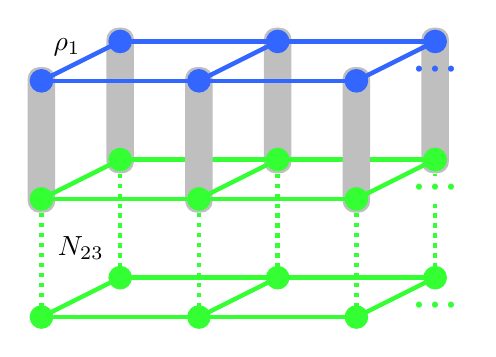
\begin{tikzpicture}[scale=0.5]
    % Define custom colors
    \definecolor{customBlue}{rgb}{0.2, 0.4, 1}
    \definecolor{customGreen}{rgb}{0.2, 1, 0.2}

    \fill[lightgray, rounded corners=0.15cm] (2-0.35,3+1-0.35) rectangle (2+0.35,6+1+0.35);
    \fill[lightgray, rounded corners=0.15cm] (6-0.35,3+1-0.35) rectangle (6+0.35,6+1+0.35);
    \fill[lightgray, rounded corners=0.15cm] (10-0.35,3+1-0.35) rectangle (10+0.35,6+1+0.35);

    \draw[customGreen, ultra thick] (0,0+0) -- (4,0+0) -- (8,0+0);  
    \draw[customGreen, ultra thick] (2,0+1) -- (6,0+1) -- (10,0+1); 
    \draw[customGreen, ultra thick] (0,0+0) -- (2,0+1);  
    \draw[customGreen, ultra thick] (4,0+0) -- (6,0+1);
    \draw[customGreen, ultra thick] (8,0+0) -- (10,0+1);

    \draw[customGreen, ultra thick] (2,3+1) -- (6,3+1) -- (10,3+1);

    \fill[lightgray, rounded corners=0.15cm] (0-0.35,3+0-0.35) rectangle (0+0.35,6+0+0.35);
    \fill[lightgray, rounded corners=0.15cm] (4-0.35,3+0-0.35) rectangle (4+0.35,6+0+0.35);
    \fill[lightgray, rounded corners=0.15cm] (8-0.35,3+0-0.35) rectangle (8+0.35,6+0+0.35);

    \draw[customGreen, ultra thick] (0,3+0) -- (4,3+0) -- (8,3+0);
    \draw[customGreen, ultra thick] (0,3+0) -- (2,3+1);
    \draw[customGreen, ultra thick] (4,3+0) -- (6,3+1);
    \draw[customGreen, ultra thick] (8,3+0) -- (10,3+1);
    
    \draw[customBlue, ultra thick] (0,6+0) -- (4,6+0) -- (8,6+0);
    \draw[customBlue, ultra thick] (2,6+1) -- (6,6+1) -- (10,6+1);
    \draw[customBlue, ultra thick] (0,6+0) -- (2,6+1);
    \draw[customBlue, ultra thick] (4,6+0) -- (6,6+1);
    \draw[customBlue, ultra thick] (8,6+0) -- (10,6+1);


    % First and second rows of disks
    \fill[customGreen] (0,0+0) circle (0.3);
    \fill[customGreen] (4,0+0) circle (0.3);
    \fill[customGreen] (8,0+0) circle (0.3);
    \fill[customGreen] (2,0+1) circle (0.3);
    \fill[customGreen] (6,0+1) circle (0.3);
    \fill[customGreen] (10,0+1) circle (0.3);

    \fill[customGreen] (0,3+0) circle (0.3);
    \fill[customGreen] (4,3+0) circle (0.3);
    \fill[customGreen] (8,3+0) circle (0.3);
    \fill[customGreen] (2,3+1) circle (0.3);
    \fill[customGreen] (6,3+1) circle (0.3);
    \fill[customGreen] (10,3+1) circle (0.3);

    \fill[customBlue] (0,6+0) circle (0.3);
    \fill[customBlue] (4,6+0) circle (0.3);
    \fill[customBlue] (8,6+0) circle (0.3);
    \fill[customBlue] (2,6+1) circle (0.3);
    \fill[customBlue] (6,6+1) circle (0.3);
    \fill[customBlue] (10,6+1) circle (0.3);

    \draw[customGreen, ultra thick, dotted] (0,0+0) -- (0,3+0);
    \draw[customGreen, ultra thick, dotted] (4,0+0) -- (4,3+0);
    \draw[customGreen, ultra thick, dotted] (8,0+0) -- (8,3+0);
    \draw[customGreen, ultra thick, dotted] (2,0+1) -- (2,3+1);
    \draw[customGreen, ultra thick, dotted] (6,0+1) -- (6,3+1);
    \draw[customGreen, ultra thick, dotted] (10,0+1) -- (10,3+1);

    \node at (10,0+0.25) [text=customGreen] {\huge \(\cdot\)\(\cdot\)\(\cdot\)};
    \node[fill=white, inner sep=0pt] at (10,3+0.25) [text=customGreen] {\huge \(\cdot\)\(\cdot\)\(\cdot\)};
    \node at (10,6+0.25) [text=customBlue] {\huge \(\cdot\)\(\cdot\)\(\cdot\)};

    \node[fill=white, inner sep=0pt] at (1,1.75) {$N_{23}$};
    \node at (0.65,6.85) {$\rho_1$};
\end{tikzpicture}
}
\caption{The estimation of entanglement witnesses for multipartite graph states.}
\label{graph state scheme}
\end{figure}

\subsection{ EWs for multipartite systems}

Thirdly, entanglement detection by state preparation can be extended to multipartite quantum states. We here, in particular, consider graph states, a class of states as a resource for MBQC \cite{PhysRevLett.86.5188}. Let us again present an instance for a three-qubit graph state, a Greenberger–Horne–Zeilinger (GHZ) state $|\psi\rangle = (|000\rangle +|111\rangle)/\sqrt{2}$ \cite{PhysRevA.62.062314}, see Fig. \ref{fig:chain}. An EW to detect a GHZ state may be given as,
\bea
W = \frac{1}{2} \mathbbm{1} - |\psi \rangle \langle \psi|.
\eea
A network state for an EW above can be constructed as,
\bea
N_{23} = \frac{1}{8} \sum_{a,b,c=0}^{1} \psi_{abc}^{(A_2 B_2 C_2)} \otimes \psi_{abc}^{(A_3 B_3 C_3)}.
\eea
where $\psi_{abc} = |\psi_{abc}\rangle \langle \psi_{abc}|$,
\bea
|\psi_{abc}\rangle = Z^a \otimes X^b \otimes X^c |\psi\rangle, ~~a,b,c \in \{0,1\}
\eea
with Pauli matrices $X$ and $Z$. It holds that
%\bea
%\tr[\rho W] =  8 \tr[\rho_1\otimes N_{23} P_{12} \otimes (\frac{\mathbbm{1}}{2} - |\psi \rangle\langle \psi |)_{3}], \nonumber
%\eea
\bea
{}_{A_3B_3C_3} \langle \psi |\rho_1 \otimes N_{23} ~P^{(12)} |\psi \rangle_{A_3B_3C_3} = \frac{1}{16} - \frac{1}{8}\tr[\rho W], \nonumber
\eea
which shows detection of a genuinely multipartite entangled state $\rho$ by finding that the left-hand-side is greater than $1/16$. Further generalization for detecting entangled $n$-qubit graph states is provided in Appendix. \\


\subsection{ To construct non-decomposable EWs }


Finally, let us investigate two entangled states defined by an EW. One denotes an entangled state $\rho_1$ detected by an EW, and the other $N_{23}$ realizing an EW by its preparation; see also Eq. (\ref{eq:ewm}). The result in Ref. \cite{PhysRevLett.96.150501} shows that an EW detects a set of entangled states that can activate its network state. Since a pair of PPT states cannot activate each other, either the states $\rho_1$ or $N_{23}$ must be non-PPT. Hence, a network state $N_{23}$ to detect a PPT entangled state $\rho_1$ should be non-PPT. We thus conclude that multipartite non-PPT entangled states can construct non-decomposable EWs, which are then highly non-trivial.
{
Note that non-PPT states can construct both decomposable and nondecomposable EWs, as shown in the example of reduction EWs, see Eq. \eqref{reductionEW}.
}
\\

{ \section{Robustness}
\label{sec:robust}

The framework for detecting entangled states in the subsection \ref{sec:gc} contains elements, the preparation of a network state and a fixed measurement for estimating a singlet fraction. We reiterate the relation between the estimation of an EW and the framework with a network state, 
\begin{align}
\tr[\rho W] = \alpha ~ \tr[\rho_1 \otimes N_{23} P^{(12)} (\eta \I - |\phi_{d}^+\rangle \langle \phi_{d}^+ | )_3 ],
\end{align}
for some $\alpha>0$. We here investigate the effect of noise on the preparation of a network state and a fixed measurement and show that the framework can unambiguously detect entangled states. That is, for separable states, the framework with noisy resources gives a non-negative expectation value. 


\begin{figure*}[t]
    \centering
    \includegraphics[scale=.18]{ fig4.pdf}
    \caption{  {Estimation of an EW in Eq. (\ref{eq:ewex}) can be realized in a circuit, where a network state in Eq. (\ref{eq:wr}) is realized and measurements in the computational basis are applied, see also Eq. (\ref{eq:ewr}). (1) A state for detecting entanglement, $|\psi^{-}\rangle$, is generated in registers $A_1B_1$. (2) A network state from an EW  is prepared to detect entanglement generated in $A_1B_1$. (3) A projection onto a state $|\phi^+\rangle $ is realized by collecting outcomes $00$ in registers $A_1A_2$. (4) A projection onto a state $|\phi^+\rangle $ is realized by collecting outcomes $00$ in registers $B_1B_2$. (5) Given outcomes $0000$ in registers $A_1B_1A_2B_2$, the singlet fraction is estimated in $A_3B_3$: a state in register $A_1B_1$ is entangled if the probability of outcomes $00$ in $A_3B_3$ is larger than $1/2$.  }}
    \label{fig:4}
\end{figure*}


\subsubsection*{ Noisy network states }
Suppose that the network states $N$ is noisy such that
\begin{align*}
\widetilde N &= (1-p) N + p \frac{\I}{d^{2n}},
\end{align*}
with some noise fraction $p$. It follows that,
\bea
&&\alpha~ \tr[\rho_1 \otimes \widetilde N_{23} P^{(12)} (\eta \I -  |\phi_{d}^+\rangle \langle \phi_{d}^+ | )_3 ] \nonumber \\
%&=&  \tr[\rho_1 \otimes ((1-p) N + p \frac{\I}{d^{2n}})_{23} P^{(12)} (\eta \I - \psi)_3 ]  \nonumber \\
&=& (1-p) \tr[\rho W] + \alpha p \frac{1}{d^{2n}} \frac{1}{d^{n}} (\eta d^n-1) \nonumber \\
&\geq & (1-p) \tr[\rho W]. \nonumber
\eea
Note that the term apart from $\tr[\rho W]$ in the second line is not negative since $\eta\leq 1/d$. Hence, noisy network states can be used to detect entangled states unambiguously. 



\subsubsection*{White noise in singlet fraction estimation}
Suppose that a fixed measurement setting for estimating a singlet fraction is noisy,
\begin{align}
(1-q)  |\phi_{d}^+\rangle \langle \phi_{d}^+ | + q \frac{\I}{d^n} \nonumber
\end{align}
with some noise fraction $q$. It follows that
\bea
&& \alpha ~ \tr[\rho_1 \otimes N_{23} P^{(12)} (\eta \I - (1-q)  |\phi_{d}^+\rangle \langle \phi_{d}^+ | - q \frac{\I}{d^n}  )_3 ]  \nonumber \\
 &= & (1-q)\tr[\rho W] + \alpha q \frac{1}{d^n} (\eta - \frac{1}{d^n} \tr[\rho^T N] ) \nonumber \\
 &\geq & (1-q) \tr[\rho W]. \nonumber
\eea
Thus, when a fixed measurement setting is noisy, the framework gives non-negative expectation values for separable states.

% \subsection{White noise in local Bell measurements}
% Now suppose that the local Bell measurements $P_{00}$ are replaced by  
% \begin{align*}
% \widetilde P = (1-r) P_{00} + r \frac{\I}{2^2}, % \label{noisy P}
% \end{align*}
% with the noise fraction $r$.
% With the noisy local Bell measurements, the state of interest $\rho$ is detected by MBEW if
% \begin{align}
% 0 &> \tr[\rho_1 \otimes N_{23} (\widetilde{P}\power{n})_{12} \otimes (\frac{1}{2}\I - \dyad{\vo}_G)^{(S'')}] \lb
% &= \tr \bigg[\rho_1 \otimes N_{23} (\frac{1}{2}\I - \dyad{\vo}_G)^{(S'')} \otimes \lb
% &\phantom{= \tr \bigg[} \left( \sum_{k=0}^{n} \binom{n}{k} q^{n-k} (\frac{1-q}{2^2})^k P_{00}\power{n-k} \otimes \I\power{k} \right)^{(SS')} \bigg] \lb
% &= \frac{1}{2^n} \tr \bigg[\rho_1 \otimes (\frac{1}{2}\I - \dyad{\vo}_G)^{(S')} \lb
% & \phantom{= \frac{1}{2^n} \tr\bigg[} \left( \sum_{k=0}^{n} \binom{n}{k} q^{n-k} (\frac{1-q}{2^2})^k P_{00}\power{n-k} \otimes \I\power{k} \right)^{(SS')} \bigg] \label{Bell noise exact}
% \end{align}
% It is too complicated to calculate exact value of the expression in the Ineq. (\ref{Bell noise exact}). Instead, let us consider an upper bound of the expression given by the worst case: the measurements are $P_{00}\power{n}$  (success) with a probability $q^n$, and $(\frac{\I}{2^2})\power n$ (fail) with a probability $1-q^n$. Then, the state $\rho$ is detected when
% \begin{align}
% \frac{1}{2^n} \left( q^n \frac{1}{2^n} \tr[\rho W] + (1-q^n) \frac{1}{2^{2n}} (\frac{1}{2} 2^n -1) \right) < 0,
% \end{align}
% which implies 
% \begin{align}
% \tr[\rho W] < (\frac{1}{2} - \frac{1}{2^n}) (1 - \frac{1}{q^n}).
% \end{align}
% }


\section{Realization in quantum circuits}


The framework of detecting entangled states by a fixed measurement can be realized in a quantum circuit. Here, we demonstrate the realization of a network state and the estimation of an EW with an example in Eq. (\ref{eq:ewex}). To facilitate the construction of a quantum circuit, we exploit a decomposition of the network state in the following, 
\begin{align}
N_{23} &= \frac{1}{4} \big( \ketbra{\psi^-}_{A_2 B_2} \otimes \ketbra{\phi^+}_{A_3 B_3}  \nonumber \\
&~~~~~~ + \ketbra{\psi^+}_{A_2 B_2} \otimes \ketbra{\psi^+}_{A_3 B_3} \nonumber \\
&~~~~~~ + \ketbra{\phi^-}_{A_2 B_2} \otimes \ketbra{\phi^-}_{A_3 B_3} \nonumber \\
&~~~~~~ + \ketbra{\phi^+}_{A_2 B_2} \otimes \ketbra{\psi-}_{A_3 B_3} \big), 
\end{align}
which is identical to the state in Eq. \eqref{eq:wr}. Then, a circuit for realizing the network state is shown in Fig. \ref{fig:4}, where blocks (1)-(5) describe realizations of a network state, projection on a state $|\phi^+\rangle$, measurements of estimating the singlet fraction. We remark that a fixed measurement setting is used for estimating an EW. 

Considering the effect of noise in Section \ref{sec:robust}, one may expect that the framework can be realized in a noisy implementation of quantum information processing. We then implemented the circuit in the IBMQ Kyiv on April 2, 2025. The results are presented in Fig. \ref{fig:result}, demonstrating the robustness of the proposed framework for estimating EWs in a realistic setting. Although noise is present, the estimation of an EW shows a singlet fraction $0.61$ higher than the threshold $1/2$, detecting the presence of an entangled state in registers $A_1B_1$.


%\begin{figure}[t]
%\centering
%\[
%\Qcircuit @C=1em @R=.7em @!R {
%\lstick{A_1} & \gate{H} & \ctrl{1} & \gate{Z} & \qw        & \qw        & \ctrl{2} & \gate{H} & \qw      & \qw      & \meter & \cw \\
%\lstick{B_1} & \qw      & \targ    & \gate{X} & \qw        & \qw        & \qw      & \qw      & \ctrl{2} & \gate{H} & \meter & \cw \\
%\lstick{A_2} & \gate{H} & \ctrl{1} & \gate{Z} & \qw        & \qw        & \targ    & \qw      & \qw      & \qw      & \meter & \cw \\
%\lstick{B_2} & \qw      & \targ    & \gate{X} & \targ      & \ctrl{0}   & \qw      & \qw      & \targ    & \qw      & \meter & \cw \\
%\lstick{A_3} & \gate{H} & \qw      & \qw      & \ctrl{-1}  & \qw        & \gate{H} & \ctrl{1} & \ctrl{1} & \gate{H} & \meter & \cw \\
%\lstick{B_3} & \gate{H} & \qw      & \qw      & \qw        & \ctrl{-2}  & \qw      & \targ    & \targ    & \qw      & \meter & \cw \\
%}
%\]
%    \caption{ The quantum circuit for detection of $\ket{\psi^-}_{A_1 B_1}$ using a pure network state $\ket{N}_{A_2B_2A_3B_3}$, which implements the EW $W = \tfrac{1}{2} \I - \psi^-$ \eqref{eq:ewex}. The first three layers in $A_1 B_1$ generate $\ket{\psi^-}$ state, while first five layers within $A_2 B_2 A_3 B_3$ generate $N$. The CNOT gates followed by $H$ gate and measurements in $A_1 A_2$ and $B_1 B_2$ implements local Bell projections. The measuremnet outcome $0000$ for the first four bits corresponds to the $\phi^+$ projections on both sides.}
 %   \label{fig:flip EW circuit}
%\end{figure}

\begin{figure}[t]
    \centering
    \includegraphics[scale=.13]{ fig5.pdf}
    \caption{ { The circuit in \ref{fig:4} is run in the IBMQ Kyiv. Given outcomes $0000$ in registers $A_1A_2B_1B_2$, the singlet fraction in registers $A_3B_3$ corresponds to the probability of having an outcome $00$. While $10000$ counts are obtained for registers $A_1A_2A_3B_1B_2B_3$, we have $685$ counts for $0000$ on $A_1A_2B_1B_2$, given which we have the singlet fraction $0.61$ which is larger than $1/2$. While the IBMQ Kyiv is noisy, we have demonstrated the generation and the detection of entangled states on a quantum circuit. 
    }}
    \label{fig:result}
\end{figure}

\section{Conclusion}


In conclusion, we have established an MB framework for estimating observables, in particular EWs, and shown the construction of network states for observables. It is also of fundamental interest to find that entanglement demonstrates elements of quantum theory, both dynamics, i.e., MBQC and observables. Our results shed new light on detecting and manipulating entangled states in a realistic scenario where precise controls via quantum gates are yet limited, such as an array of superconducting qubits, neutral atoms, or photons, where the preparation of a multipartite state and a fixed measurement are readily experimentally feasible. The results also open a new avenue of exploiting entangled states in distributed quantum information processing such as computing and metrology where entanglement is resourceful and quantum estimation {\it per se} corresponds to computing or metrology. 

In future directions, it would be interesting to realize the estimation of EWs via network states experimentally by considering the effects of noise in a realistic setting. Note that some network states, such as Smolin, have been realized in experiment \cite{Amselem:2009aa, PhysRevLett.105.130501, PhysRevLett.109.040501}. It is also interesting to exploit network states in a network and security scenario such as a measurement-device-independent scenario, see Refs. \cite{PhysRevLett.108.200401,PhysRevLett.110.060405}, so that observables such as EWs are estimated by relaxing assumptions on joint measurements; estimation of EWs, as well as detection of entanglement, is achieved in a higher level of robustness against imperfect implementations. 

\section*{Acknowledgement}

This work is supported by National Research Foundation of Korea (NRF-2021R1A2C2006309, NRF-2022M1A3C2069728) and the Institute for Information \& Communication Technology Promotion (IITP) (RS-2023-00229524, the ITRC Program/IITP-2023-2018-0-01402). AB and DC were supported by the Polish National Science Center project No. 2018/30/A/ST2/00837.


\bibliographystyle{quantum}
% \bibliography{bibedsp}
% \documentclass[a4paper,twocolumn,11pt,accepted=2017-05-09]{quantumarticle}
\documentclass[a4paper,twocolumn,10pt]{quantumarticle}
\pdfoutput=1
\usepackage[utf8]{inputenc}
\usepackage[english]{babel}
\usepackage[T1]{fontenc}
\usepackage{amsmath}
\usepackage{hyperref}

\usepackage{tikz}
\usepackage{lipsum}

\newtheorem{theorem}{Theorem}


\usepackage{tikz}
\usepackage{qcircuit}
%%%%%%%%%%%%%%%%%%

%\usepackage{IEEEtrantools}
\usepackage{multirow}

% ------------------------------------------------------------------------------
\newcommand{\rev}{\color{blue}}
\newcommand{\bae}{\color{purple}}
\newcommand{\ji}{\color{gray}}

\newcommand{\vx}{\Vec{x}}
\newcommand{\vy}{\Vec{y}}
\newcommand{\vo}{\Vec{0}}
\newcommand{\Va}{\Vec{a}}
\newcommand{\Vb}{\Vec{b}}
\newcommand{\power}[1]{^{\otimes #1}}
\newcommand{\lb}{\nonumber \\}


\newcommand{\R}{\mathbb{R}}
\newcommand{\N}{\mathbb{N}}
\newcommand{\C}{\mathbb{C}}
\newcommand{\Z}{\mathbb{Z}}
\newcommand{\Q}{\mathbb{Q}}
\newcommand{\I}{\mathbbm{1}}

\newcommand{\tr}{\text{tr}}
\newcommand{\ket}[1]{| #1 \rangle}
\newcommand{\bra}[1]{\langle #1|}
\newcommand{\ip}[2]{\langle #1|#2 \rangle}
\newcommand{\bracket}[3]{\langle #1|#2|#3 \rangle}
\newcommand{\sm}[1]{\left( \begin{smallmatrix} #1 \end{smallmatrix} \right)}

\newcommand{\be}{\begin{equation}}
\newcommand{\ee}{\end{equation}}
\newcommand{\bea}{\begin{eqnarray}}
\newcommand{\eea}{\end{eqnarray}}
\newcommand{\bes}{\begin{equation*}}
\newcommand{\ees}{\end{equation*}}
\newcommand{\beas}{\begin{eqnarray*}}
\newcommand{\eeas}{\end{eqnarray*}}

% ------------------------------------------------------------------------------

\newcommand{\x}{\mathrm{x}}
%\newcommand{\ket}[1]{|#1\rangle}
\newcommand{\ketbra}[1]{\ket{#1}\!\bra{#1}}
%\newcommand{\bra}[1]{\langle#1|}
\newcommand{\dyad}[1]{\ket{#1}\!\bra{#1}}

\newcommand{\ten}{\otimes}
\newcommand{\Id}{\mathds{1}}
\newcommand{\zero}{\mathbf{0}}
\newcommand{\KBDS}{C^{s}}
\newcommand{\KBDSs}{C}
%\newcommand{\KBDS}{C^{\mbox{\tiny U}}}
\newcommand{\KTwo}{C^{2\times2}}
\renewcommand{\H}{\mathcal{H}}
\def\A{\mathcal{A}}
\def\B{\mathcal{B}}

\def\x{\mathrm{x}}
\def\y{\mathrm{y}}

\def\W{\mathcal{W}}


\def\sig{\widetilde{\sigma}}
\def\F{\mathcal{F}}
\def\N{\mathcal{N}}
\def\P{\mathbbm{P}}
\def\tr{\mathrm{tr}}

\def\L{\mathcal{L}}
\def\Q{\mathcal{Q}}
\def\NL{\mathcal{NS}}

\DeclareMathOperator*{\Oplus}{\bigoplus}
\DeclareMathOperator*{\Otimes}{\bigotimes}
% \DeclareMathOperator*{\Oplus}{\scalerel*{\bigoplus}{\textstyle\sum}}
% ------------------------------------------------------------------------------






\begin{document}

\title{ Detecting Entanglement by State Preparation and Local Measurements}


\author{Jaemin Kim}
\email{woals6584@kaist.ac.kr}
\affiliation{School of Electrical Engineering, Korea Advanced Institute of Science and Technology (KAIST), 291 Daehak-ro, Yuseong-gu, Daejeon 34141, Republic of Korea }
\orcid{ }


\author{Anindita Bera}
\email{aninditatitli@gmail.com}
\affiliation{Department of Mathematics, Birla Institute of Technology Mesra, Jharkhand 835215, India}
\orcid{ }


\author{Dariusz Chru\'sci\'nski}
\email{darch@fizyka.umk.pl}
\affiliation{Institute of Physics, Faculty of Physics, Astronomy, and Informatics, Nicolaus Copernicus University, Grudziadzka 5, 87-100 Torun, Poland}
\orcid{ }

\author{Joonwoo Bae}
\email{joonwoo.bae@kaist.ac.kr}
\affiliation{School of Electrical Engineering, Korea Advanced Institute of Science and Technology (KAIST), 291 Daehak-ro, Yuseong-gu, Daejeon 34141, Republic of Korea }
\orcid{ }


\maketitle

\begin{abstract}
  Entanglement witnesses (EWs) are a collection of observables that can characterize separable states and, experimentally, estimating EWs can verify entangled states. In this work, we show that a fixed measurement setting on a multipartite entangled state, which we introduce as a \emph{network state} for the purpose, can estimate EWs. Namely, entangled states can be fully verified in a measurement-based manner, in which experimenters do not necessarily change measurement settings. We present a fixed measurement setting and network states for estimating decomposable EWs, equivalent to the partial transpose criteria. We also consider non-decomposable EWs that detect bound entangled states beyond the partial transpose criteria. The results can be extended to multipartite states such as graph states, a resource for measurement-based quantum computing, and readily applied to distributed settings such as quantum metrology or sensor networks where multipartite entangled states are resourceful.
\end{abstract}





\section{Introduction}


{Entangled states are a key resource in quantum information processing, in particular, to achieve quantum advantages in computation and communication tasks. A higher level of security in cryptographic protocols \cite{PhysRevLett.98.230501}, higher level of quantum certification \cite{Pironio_2009, PhysRevLett.110.060405, PhysRevLett.108.200401, Bowles:2018aa} and higher network channel capacities \cite{PhysRevA.95.052329, PhysRevLett.125.150502} can be achieved by exploiting entangled states. Efficient computation with quantum resources can be realized by local measurements and entangled states only, called measurement-based quantum computation (MBQC) \cite{PhysRevLett.86.5188, MeasurementBasedQuantumComputation, Briegel:2009aa}. }

{ Entanglement witnesses (EWs) \cite{TERHAL2000319, PhysRevA.62.052310} are versatile tools to detect entangled states both theoretically and experimentally. They correspond to observables that are non-negative for all separable states but negative for some entangled states \cite{HORODECKI19961, GUHNE20091, RevModPhys.81.865, Chru_ci_ski_2014, Friis:2019aa}. Hence, negative expectation values of EWs unambiguously conclude the presence of entangled states. In practice, multiple measurement settings may be necessary for estimating EWs. }

{ In this work, we show that a fixed measurement setting can detect entangled states, together with the preparation of a multipartite state, which we call a {\it network state}. To be precise, we present a framework for detecting entangled states such that a fixed measurement over a network state $N$ and a state $\rho$ can find if the state $\rho$ is entangled, where a network state $N$ is obtained from an EW. Thus, entangled states can be verified in a measurement-based (MB) manner. In fact, the framework is closely connected to the activation of entanglement in that it finds if a state $\rho$ is entangled if a joint state $N\otimes \rho$ is more entangled than a state $N$. }

We show how network states can be obtained from EWs. We present the construction of network states for decomposable EWs, which are equivalent to the partial transpose criteria, and also for non-decomposable EWs that detect bound entangled states beyond the partial transpose criteria, such as the Bell-diagonal EWs \cite{chruscinski2014class, PhysRevA.105.052401} from the Choi map \cite{Choi:1975aa} and its various generalizations \cite{PhysRevA.84.024302}, and the Breuer-Hall EW \cite{PhysRevLett.97.080501, Hall_2006}. The results are extended to multipartite systems: graph states \cite{PhysRevA.69.062311}, a resource for MBQC \cite{PhysRevLett.86.5188}, can be detected by network states and a fixed measurement.
{ 
We discuss the connection of our work to the entanglement activation \cite{PhysRevLett.96.150501} and the measurement-device-independent entanglement witnesses \cite{PhysRevLett.110.060405}.
}

The importance of our results is threefold. Firstly, similarly to MBQC, one can circumvent the control of multiple measurement settings when estimating observables. Precise controls on and the preparation of general measurements identify additional difficulties for realizing EWs in general. Our results show that the preparation of quantum states and a fixed measurement can be an experimentally feasible alternative. Secondly, it is of fundamental interest to find that entangled states with a fixed measurement are a resource that can be replaced with observables. Note that MBQC signifies that entangled states and local measurements can be an alternative to realize quantum state transformation. Finally, the framework for estimating EWs in an MB manner finds various usefulness of distributed settings such as distributed quantum metrology over networks, e.g., \cite{Chabuda:2020aa, Zhang_2021,Len:2022aa, PhysRevLett.121.043604}: estimation of joint observables enables distributed quantum information processing, e.g., \cite{PhysRevA.85.062326, Friis_2017, PhysRevLett.120.080501}.

\section{Entanglement detection}
 
Let us begin by describing an experimental scenario of verifying entangled states, where the scenario is common in various experimental settings. We consider two quantum systems $A$ and $B$ on a Hilbert space $\H\otimes \H$. Interestingly, observables exist, denoted by $W=W^{\dagger}$, such that, for all separable states $\sigma_{\mathrm{sep}}$, 
\bea
\tr[W\sigma_{\mathrm{sep}}] \geq 0~~\mathrm{and }~~ \tr[W\rho_{\mathrm{ent}}] <0\nonumber
\eea
for some entangled states $\rho_{\mathrm{ent}}$ \cite{TERHAL2000319, PhysRevA.62.052310}. All entangled states can be verified by estimating some observables, which are called entanglement witnesses (EWs). In experiment, EWs can be estimated by altering measurement settings in general: negative expectation values unambiguously conclude entangled states \cite{GUHNE20091}. They can be also used to verify other properties, other than entanglement, such as a fidelity in the state preparation \cite{PhysRevA.76.030305, Haffner:2005aa}.

%Note that the structure of EWs remains } 


%One of the intriguing properties of entangled states is the irreversibility in manipulations of entanglement. Entangled states from which no entanglement can be extracted, though entanglement is needed for their preparation, are identified as {\it undistillable} or {\it bound} entangled states \cite{PhysRevA.61.062313, PhysRevLett.86.2681}. Multipartite quantum states that remain positive after partial transpose (PPT) turn out to be undistillable. Remarkably, PPT entangled states can be used to activate other entangled states \cite{horodecki1999bound}.

%Then, non-PPT entangled states can be characterized by decomposable EWs that have a general form as follows,
%\bea
%W = P+Q^{\Gamma},~~\mathrm{for}~~P,~Q\geq 0\nonumber.
%\eea
%Here $\Gamma$ denotes the partial transpose. Then, non-decomposable EWs, which cannot be in the form above, can detect PPT entangled states. 

%\cite{PhysRevA.61.062313, PhysRevLett.86.2681}.

%In general, it is highly non-trivial to construct non-decomposable EWs, which are the main object in the mathematically challenging problem of classifying positive linear maps of Operator Algebras \cite{Stormer:1963aa}, see also Refs. \cite{bera2022generalizing, bera2022class,mirror}.

{\section{Measurement-Based Estimation}

Let us show that observables can be generally estimated in a measurement-based manner. We here focus on EWs, observables of particular interest for detecting entangled states, and provide the scheme for estimating of single observables in Appendix. We devise multipartite quantum states, {\it called network states}, for estimating observables. 

\subsection{Example }
\label{subsec:ex}
Let us begin with an illuminating example of an MB estimation of an EW. Throughout, Bell states are denoted by $|\phi^{\pm}\rangle = (|00\rangle \pm |11\rangle)/\sqrt{2}$ and $|\psi^{\pm}\rangle = (|01\rangle \pm |10\rangle)/\sqrt{2}$. We consider an EW in the following,
\bea
%W = \frac{1}{2} \mathbbm{1} - |\psi^{-} \rangle \langle \psi^{-} |, \nonumber
W = \frac{1}{4} (\mathbbm{1} + X\otimes X + Y\otimes Y + Z\otimes Z) \label{eq:ewex}
\eea
where $X,Y$ and $Z$ are Pauli matrices. Eq. (\ref{eq:ewex}) shows that an EW can be estimated by various measurement settings. Note that a Bell state $|\psi^{-}\rangle$ is detected by an EW above. 
 
 
%\subsection{Two-qubit network states}

The MB framework for estimating an observable in Eq. (\ref{eq:ewex}) can be achieved by a four-partite state, called a {\it network state}, constructed as follows, 
\bea
N_{23} &=& \frac{1}{4} |\psi^-\rangle_{A_2B_2} \langle \psi^-| \otimes |\phi^+\rangle_{A_3B_3} \langle \phi^+| + \nonumber \\
&&\frac{1}{12} (\mathbbm{1} - |\psi^-\rangle_{A_2B_2} \langle \psi^-|) \otimes (\mathbbm{1} - |\phi^+\rangle_{A_3B_3} \langle \phi^+|),~~~~ ~\label{eq:wr}
\eea

on sites $A_2A_3B_2B_3$, see Fig. \ref{fig:fig1}. We then place a state of interest at $A_1B_1$, denoted by $\rho_{1}:=\rho^{( A_1B_1)}$, which we want to learn if it is entangled. We have
\bea
\tr[\rho W ] =  16~ \tr  [\rho_1\otimes N_{23} (\frac{1}{2}\mathbbm{1} - | \phi^+\rangle_{A_3B_3} \langle \phi^+|) \otimes P^{(12)}],~~
\label{eq:ewr}
\eea
where $P^{(12 )} = |\phi^{+}\rangle_{A_1A_2}\langle \phi^+| \otimes |\phi^{+}\rangle_{B_1B_2}\langle \phi^+|$. Eq. (\ref{eq:ewr}) can be simplified by a singlet fraction as follows,
\bea
_{A_3 B_3}  \langle \phi^{+}| \tr_{12}[ \rho_1 \otimes N_{23} ~P^{(12)} ]  |\phi^{+}\rangle_{A_3 B_3}   = \frac{1}{8} - \frac{1}{4}\tr[\rho W].~~
\label{eq:expew}
\eea
The left-hand-side can be obtained by preparing a network state followed by a fixed measurement. A state $\rho_1$ is entangled if the right-hand-side is greater than $1/8$ since $\tr[\sigma_{\mathrm{sep}}W ]\geq 0 $ for all separable states $\sigma_{\mathrm{sep}}$. Once a Bell measurement reports an outcome $P^{(12)} $, a singlet fraction is estimated from the probability of having outcome $|\phi^{+}\rangle$ on $A_3B_3$. Thus, it is shown that an EW can be estimated in a fully MB manner. 

%In fact, an entangled state $\rho$ is detected if the probability, i.e., the left-hand-side in Eq. (\ref{eq:expew}), is greater than $1/8$, since $\tr[\sigma_{\mathrm{sep}}W ]\geq 0 $ for all separable states $\sigma_{\mathrm{sep}}$.


Experimental resources to realize the MB framework, i.e., the left-hand side in Eq. (\ref{eq:expew}), are as follows. A network state is required, see Eq. (\ref{eq:ewex}), which is entangled and bi-separable. The detection scheme needs a measurement in the basis $|\phi^+\rangle$, which is equivalent to the capability of realizing a controlled-NOT gate, a Hadamard gate, and a fixed-measurement in the $z$-direction; see also Fig. \ref{fig:fig1}. All these are compatible with the resources to realize MBQC. In addition, it is worth mentioning that a network state in Eq. (\ref{eq:wr}) is a variation of a Smolin state, a four-partite bound entangled state \cite{PhysRevA.63.032306}, which has been repeatedly realized in experiment \cite{ Amselem:2009aa, PhysRevLett.105.130501, PhysRevLett.109.040501}. It should be pointed out that a realization of the presented MB framework is readily available in an experiment. 



\begin{figure}[t]
\centering
% \includegraphics[width=9.0cm ]{figure1}
\resizebox{0.9\linewidth}{!}{
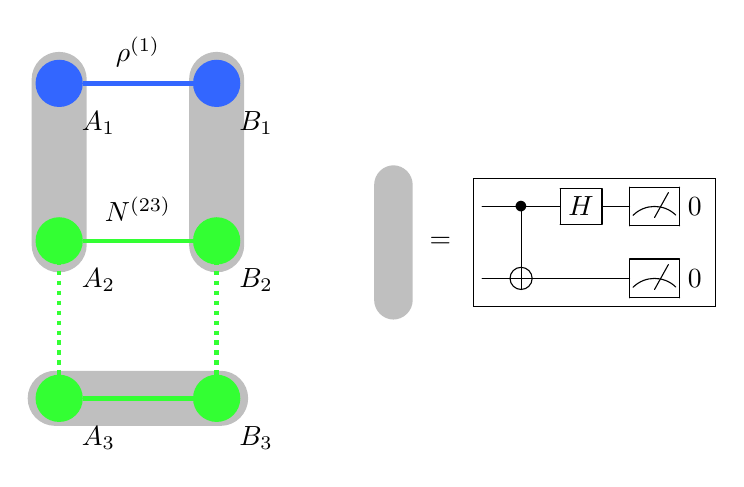
\begin{tikzpicture}[scale=2]
    % Define custom colors
    \definecolor{customBlue}{rgb}{0.2, 0.4, 1}
    \definecolor{customGreen}{rgb}{0.2, 1, 0.2}

    % Round-edged rectangles and dotted lines for both rows
\fill[lightgray, rounded corners=0.35cm] (-0.175,1.2) rectangle (0.175,-0.2);
\fill[lightgray, rounded corners=0.35cm] (-1-0.175,1.2) rectangle (-1+0.175,-0.2);
\fill[lightgray, rounded corners=0.35cm] (-0.5-0.7,-0.825) rectangle (-0.5+0.7,-1.175);
\draw[customGreen, ultra thick, dotted] (0,0) -- (0,-1);
\draw[customGreen, ultra thick, dotted] (-1,0) -- (-1,-1);

% Green ultra thick lines between A2-B2 and A3-B3
\draw[customGreen, ultra thick] (0.15,0) -- (-1+0.15,0);
\draw[customGreen, ultra thick] (0.15,-1) -- (-1+0.15,-1);

% Blue ultra thick line between A1 and B1
\draw[customBlue, ultra thick] (0.15,1) -- (-1+0.15,1);

    % First row of disks
    \fill[customBlue] (0,1) circle (0.15);
    \fill[customGreen] (0,0) circle (0.15);
    \fill[customGreen] (0,-1) circle (0.15);

    % Second row of disks
    \fill[customBlue] (-1,1) circle (0.15);
    \fill[customGreen] (-1,0) circle (0.15);
    \fill[customGreen] (-1,-1) circle (0.15);

    % Captions
    \node at (-0.5,1.2) {$\rho^{(1)}$};
    \node at (-0.5,0.2) {$N^{(23)}$};

% Labels
\node at (-1+0.25,0.75) {$A_1$};
\node at (-1+0.25,-0.25) {$A_2$};
\node at (-1+0.25,-1.25) {$A_3$};
\node at (+0.25,0.75) {$B_1$};
\node at (+0.25,-0.25) {$B_2$};
\node at (+0.25,-1.25) {$B_3$};

    \begin{scope}[xshift=1cm, yshift=-0.5cm, scale=0.7] % Adjust yshift for spacing between figures
        \fill[lightgray, rounded corners=0.25cm] (0,0) rectangle (0.35,1.4);

        \node at (0.6,0.7) {$=$};

        % Quantum Circuit inside a TikZ node
        \node[draw, inner sep=3pt] at (2,0.7) {
            \Qcircuit @C=1em @R=1.2em {
            % Qubit setup
            \lstick{} & \ctrl{1} & \gate{H} & \meter & \rstick{\hspace{-1.2em} 0} \\
            \lstick{} & \targ    & \qw      & \meter & \rstick{\hspace{-1.2em} 0} \\
            }
        };
    \end{scope}
\end{tikzpicture}
}
\caption{ A four-partite network state $N_{23}$ is prepared on $A_2A_3B_2B_3$ to detect an entangled state on $A_1B_1$. Bi-interactions and measurements in the computational basis can construct EWs, see also Eq. (\ref{eq:expew}) in the text. Gray boxes denote a measurement in the basis $|\phi^{+}\rangle$, which is equivalent to a measurement in the computational basis after applying of a controlled-NOT gate followed by a Hadamard gate. }
\label{fig:fig1}
\end{figure}



\subsection{ EWs via entanglement activation}

To show a general construction of network states for arbitrary EWs for high-dimensional quantum systems, we want to clarify their relations to activation of entanglement \cite{PhysRevLett.96.150501}: all EWs can be expressed in the following form, }
\bea
W_{A_2 B_2 } = \tr_{A_3B_3} \big[N (\eta \mathbbm{I} - |\phi_{d}^+ \rangle_{A_3B_3} \langle \phi_{d}^+ |)\big], \label{eq:ewm}
\eea
for some network state $N := N^{(A_2 B_2 A_3 B_3)}$ and a parameter $\eta \in [1/d,1 )$, where $|\phi_{d}^+\rangle = \sum_{j=0}^{d-1}|jj\rangle /\sqrt{d}$. It is worth mentioning an EW above shares similarity with Eq. (\ref{eq:ewr}) Note that the parameter $\eta$ satisfies the condition, $\eta\geq E_d [N]$ where $E_d$ is called a maximal singlet fraction,
\bea
E_d[N] &=& \sup_{\F}~ \langle \phi_{d}^+| \F[ N ] |\phi_{d}^+\rangle ~\mathrm{for~a~local ~filtering~}\F   \nonumber \\
&& \F[N] = \frac{ K_{A}\otimes K_B N K_{A}^{\dagger}\otimes K_{B}^{\dagger} }{ \tr[  K_{A}^{\dagger}K_{A} \otimes K_{B}^{\dagger}K_{B} N ]},\label{eq:fil}
\eea
where $K_A: \H_{A_1A_2}\rightarrow \mathbbm{C}^d $ and $K_B: \H_{B_1B_2}\rightarrow \mathbbm{C}^d $. It is worth mentioning that EWs in Eq. (\ref{eq:ewm}) identify entangled states that activate a network state in the sense that
\bea
E_d[ \sigma\otimes N]>\eta, ~\mathrm{whereas}~ {E_d [N]\leq \eta}.\label{eq:ac}
\eea
In fact, all entangled states can be used to activate some other state: in Eq. (\ref{eq:ac}) a state $\sigma$ is entangled if and only if it can activate some other entangled state $N$.



{ 
\subsection{ Detection protocol from  entanglement activation}

We exploit the scenario of activating entanglement as a framework for detecting entangled states. Namely, a state $\rho$ is entangled if it can be used to activate a state $N$. To this end, we consider a local filtering operation $\Phi$ as follows,
\begin{align}
\Phi (\rho \otimes N) = \tr_{A_1 B_1 A_2 B_2}[ P^{(12)} \rho^{(A_1 B_1)} \otimes N^{(A_2 B_2 A_3 B_3)}]. \nonumber
\end{align}
where $P^{(12)}$ the projection onto maximally entangled states as follows,
\bea
P^{(12 )} = |\phi_{d}^{+}\rangle_{A_1A_2}\langle \phi_{d}^+| \otimes |\phi_{d}^{+}\rangle_{B_1B_2}\langle \phi_{d}^+| \label{eq:projd} 
\eea
and $|\phi_{d}^+\rangle = \sum_{i=1}^d|ii\rangle/\sqrt{d}$. The singlet fraction after the filtering operation is given by,
\begin{align}
F_{\Phi}(\rho \otimes N) = \frac{ \bracket{\phi_d^+}{\Phi(\rho \otimes N)}{\phi_d^+} }{\tr[\Phi(\rho \otimes N)]}.\nonumber
\end{align}
With the specific local operation, the singlet fraction of a network state $N$ can be computed as, 
\begin{align}
\widetilde E_d(N) = \sup_{\sigma \in \mathrm{SEP}} F_{\Phi}(\sigma \otimes N),
\end{align}
where $\mathrm{SEP}$ denotes the set of separable states. It is clear that $\widetilde E_d(N) \le E_d(N)$ since a specific local operation is considered. Note also that for $\eta \in [\frac{1}{d},1)$, there exists a state $N$ such that $E_d(N) = \widetilde E_d(N) = \eta$ \cite{PhysRevLett.96.150501}. It holds that a state $\rho$ is entangled if we have $F_{\Phi}(\rho \otimes N) > \eta $ for $N$ such that $\widetilde E_d(N) \leq \eta$. 
}




\subsection{ General construction of network states }
\label{sec:gc}

Let us then present a construction of a network state for a given EW, see also Eq. (\ref{eq:ewm}). Suppose that an EW on $d\otimes d$ is decomposed as follows,
\bea
W = \sum_{j} a_j W(j)^T ~\mathrm{with}~ W(j) \geq 0 ~\mathrm{and}~ a_j \in \mathbbm{R}, \label{eq:eeww}
\eea
so that one can choose normalized non-negative operators $\{ \Pi(i) \geq 0\}$ and real constants $\{ c_j\}$ such that,
\bea
N_{23} &=&\sum_{j} c_j  W(j)_{A_2B_2} \otimes  \Pi(j)_{A_3B_3}, ~\mathrm{and}  \label{eq:ns} \\
W_2 & =& ~ k \, \tr_{3} [N_{23}^{T_2}  ( \eta \mathbbm{1} - |\phi_{d}^+ \rangle_{A_3B_3} \langle \phi_{d}^+ |  )  ], \label{eq:ewn}
\eea
for some $\eta\geq 1/d$ and $k>0$, where $W_2$ reproduces a given EW in Eq. (\ref{eq:eeww}) on sites $A_2 B_2$. One can find $\{a_j\}$ and $\{c_j \}$ are related as follow,
\bea
a_j = k \, c_j (\eta - \bracket{\phi_{d}^+}{\Pi(j)}{\phi_{d}^+}).\nonumber
\eea
Then, for a state $\rho_1 = \rho^{(A_1B_1)}$ it holds that
\bea
\tr[\rho W] %&=& d^2 ~ \tr[\rho_1 \otimes W_{2}^T P^{(12)}  ]  \nonumber\\
&\propto& \tr[\rho_1 \otimes N_{23} ~ P^{(12)} \otimes ( \eta \mathbbm{1} - |\phi_{d}^+ \rangle_{A_3B_3} \langle \phi_d^+ |  ) ]. ~~~~~ \label{eq:m}
\eea
For an entangled state $\rho$ detected by $W$, i.e., $\tr[\rho W]<0$, Eq. (\ref{eq:m}) shows that
\bea
\eta &<&  _{A_3B_3}\langle \phi_{d}^+| \Lambda^{(1\rightarrow 3)} [\rho_1]|\phi_{d}^+\rangle_{A_3B_3} \nonumber \\
&&\mathrm{where}~ \Lambda^{( 1\rightarrow 3)} [\rho_1]= \frac{ \tr_{12}[\rho_{1}\otimes N_{23} P^{(12)}] }{ \tr[\rho_1\otimes N_{23} P^{(12)}]  }. ~~\label{eq:v}
\eea
Note that the construction above applies to all EWs in general.\\

{
{\it Example.} A straightforward and facile construction of a network state from an EW is as follows. For an EW, we find a decoposition,
\bea
 W = a_+ W_+^T - a_- W_-^T\nonumber
 \eea
with coefficients $a_{\pm} > 0$ and quantum states $W_{\pm}$ (i.e., $W_{\pm} \ge 0$ and $\tr[W_{\pm}]=1$). We choose $\eta = 1/d$ and find a network state as follows,
\begin{align}
N_{23} &=c_+ W_+ \otimes \frac{\I-\dyad{\phi^+_d}}{d^2-1} +  c_- W_- \otimes \dyad{\phi^+_d}.\nonumber
\end{align}
where
\bea
c_+ = \frac{(d-1)a_+}{(d-1)a_+ + a_-} ~~\mathrm{and} ~~c_-= \frac{a_-}{(d-1)a_+ + a_-}. \nonumber
\eea 
We have presented a straightforward one by exploiting a spectral decomposition of an EW. We also stress that a network state is not unique for an EW. \\
}

A quantum teleportation protocol may rephrase Eq. (\ref{eq:v}) as follows. Once a measurement $P^{(12)}$ is successful, a state $\rho$ prepared at $A_1B_1$ is teleported at $A_3B_3$ via a network state $N_{23}$. Note that the map in Eq. (\ref{eq:v}) is a probabilistic operation assisted by entanglement \cite{PhysRevA.64.012317}; to be precise, successful Bell measurements define a channel for a state $\rho_1$ \cite{Jamiokowski:1972aa, Choi:1975aa}. Finally, a singlet fraction is estimated and compared with $\eta$, see Eq. (\ref{eq:v}), to verify entanglement. We have shown that, given an EW, one can always construct a network state for the estimation as above. 

As mentioned, experimental resources for the realization contain preparing a network state and Bell measurements that require bi-interactions and a fixed local measurement setting; see also Fig. \ref{fig:fig1}. In Appendix, we reproduce a network state in Eq. (\ref{eq:wr}) by applying the general construction above.

{
\subsection{ Noisy local projections on $A_1A_2$ and $B_1B_2$: semi measurement-device-independent entanglement witnesses } 
\label{semi MDI}

The framework of detecting entanglement relies on projections to maximally entangled states, see Eq. (\ref{eq:projd}). It bears some similarity with the measurement-device-independent (MDI) scenario \cite{PhysRevLett.108.200401,PhysRevLett.110.060405}, which applies when one wants to relax the assumption to trust measurement devices. Then, an MDI scenario trusts on state preparations and relaxes the assumptions on joint measurements. 

Similarly, we here show that projections on  $A_1A_2$ and $B_1B_2$, joint measurements performed locally, can be relaxed for the verification of entangled states. To this end, we show that untrusted joint measurements on $A_1A_2$ and $B_1B_2$ can unambiguously conclude entangled states. Let us consider a separable state $\sigma = \sum_k p_k \tau_k \otimes \xi_k$ and a threshold  $\eta$. Let $Q^{(A_1 A_2)}$ and $R^{(B_1B_2)}$ denote unknown positive-operator-valued-measure elements that may describe detection events of untrusted measurement devices. It suffices to show that $\sigma$ cannot increase the singlet fraction of $N$ larger than the threshold $\eta$. This means, 
\bea
\tr[(Q^{(A_1 A_2)} \otimes R^{(B_1 B_2)} \sigma_1 \otimes W_{2}^T]  \geq 0 \nonumber
\eea
for all $Q$ and $R$, see also $W_{2}^T$ in Eq. (\ref{eq:ewn}). We then have: 
\bea
&& \sum_k p_k \tr[(Q^{(A_1 A_2)} \otimes R^{(B_1 B_2)}) (\tau_k^{(A_1)} \otimes \xi_k^{(B_1)}) W_{2}^T ] \nonumber \\
%&=& \sum_k p_k \tr[(\widetilde{Q}^{(A_2)} \otimes \widetilde{R}^{(B_2)}) N_{23} (\eta \I - \dyad{\phi^+_d})_3] \nonumber \\
%&\propto \sum_k p_k \tr[(\widetilde{Q} \otimes \widetilde{R})_2 W^T_2] \nonumber\\
&\propto& \sum_k p_k \tr[(\widetilde{Q}^T \otimes \widetilde{R}^T) W] \ge 0 \nonumber 
\eea
since 
\begin{align*}
\widetilde{Q}^{(A_2)} &= \tr_{A_1}[Q^{(A_1 A_2)} (\sigma_k^{(A_1)} \otimes \I^{(A_2)})] \ge 0, \\
\widetilde{R}^{(B_2)} &= \tr_{B_1}[R^{(B_1 B_2)} (\xi_k^{(B_1)} \otimes \I^{(B_2)})] \ge 0\nonumber
\end{align*}
and an EW is non-negative for all separable states. Hence, we have shown that joint measurements on $A_1A_2$ and $B_1B_2$ with untrusted measurements can also unambiguously conclude entangled states. 
}

\section{Examples}


Let us apply the general construction of network states and present network states for EWs known so far, such as decomposable and non-decomposable instances, the latter of which are highly non-trivial in Quantum Information Theory. Identifying all EWs is equivalent to characterizing the set of separable states, which is a challenging mathematical problem \cite{Stormer:1963aa}; the computational complexity also belongs to NP-Hard \cite{10.1145/780542.780545}. The construction of network states applies to all EWs. In what follows, we apply the general construction of network states to non-trivial EWs.

To this end, let $P_{st}$ denote a projection onto a Bell state, for $s,t = 0,\ldots, d-1$, in a dimension $d$,
\bea
P_{st} = |\phi_{st}\rangle \langle \phi_{st}| ~\mathrm{where}~|\phi_{st} \rangle = \frac{1}{\sqrt{d}} \sum_{j = 0}^{d-1} \omega^{t j } \ket{j } \ket{j + s}, ~~ \label{eq:1}
\eea
where $\omega = e^{2\pi i/d}$.
Projectors onto symmetric and anti-symmetric subspaces are denoted by $S_d$ and $A_d$, respectively,
\bea
S_d = \frac{\mathbbm{1+F} }{2}~~\mathrm{and} ~~A_d = \frac{\mathbbm{1 - F} }{2},
\eea
where $\mathbbm{F} = d P_{00}^{\Gamma}$ is a flip operator and $\Gamma$ denotes the partial transpose \cite{PhysRevA.61.062313}. Note that $\tr[A_d]=d(d-1)/2$ and $\tr[S_d] = d(d+1)/2$. Interestingly, high-dimensional Bell states and projections onto symmetric and anti-symmetric subspaces suffice to construct network states for known non-decomposable maps.



\subsection{ Decomposable EWs: the partial transposition }

Firstly, we consider a decomposable EW $W = Q^\Gamma$ for $Q\geq 0$ and $\tr[Q]=1$, for which a network state can be constructed as follows. We write by $\lambda:=\max_{i}|\lambda_i|$ where $\{\lambda_i\} $ are eigenvalues of an EW $W$ and a network state is obtained as,
\bea
N_{23}&=& c_1\left( \frac{\lambda\mathbbm{1} - Q^\Gamma }{\lambda d^2 - 1 }\right)^{(2)} \otimes P_{00}^{(3)} \nonumber\\
&&+ c_2 \left( \frac{ \lambda \mathbbm{1} +  Q^{\Gamma} }{\lambda d^2 + 1}\right)^{(2)} \otimes \left( \frac{\mathbbm{1} - P_{00}}{d^2 - 1}\right)^{(3)}, \label{eq:nsd}
\eea
where superscript $(j)$ stands for systems $A_jB_j$ and
\bea
c_1 = \frac{d^2 \lambda - 1}{d^3 \lambda  + d -2} ~~\mathrm{and}~ ~ c_2 =\frac{(d-1)(d^2 \lambda +1)}{d^3 \lambda  +d-2}. \nonumber
\eea
In the other way around, from a network state $N_{23}$ in Eq. (\ref{eq:nsd}) one can reproduce a decomposable EW, see Eq. (\ref{eq:ewm})
\bea
\tr_3[ N_{23 } (\frac{1}{d} \mathbbm{1} - |\phi_{00}\rangle_{A_3B_3}\langle \phi_{00}|)] = \frac{2(d-1)}{d(d^3 \lambda + d -2)} Q^\Gamma \propto Q^\Gamma.\nonumber
% \\ \tr_3[ N_{23}^{(\mathrm{BH})}~ (\frac{1}{d} \mathbbm{1} - |\phi_{00}\rangle_{A_3B_3}\langle \phi_{00}|)] = \frac{2(d-1)}{d(d^3 \lambda + d -2)} Q^\Gamma \propto Q^\Gamma.\nonumber
\eea
Hence, the partial transpose criteria \cite{PhysRevLett.77.1413} can be generally realized by preparing a network state with a fixed measurement.

As an instance, a network state for the decomposable and optimal EW $W = P_{00}^{\Gamma}$ can be found as
\bea
\frac{1}{d+2} \left( \frac{A_d}{\tr A_d} \right)^{(2)} \otimes P_{00}^{(3)}  +  \frac{d+1}{d+2} \left( \frac{S_d}{\tr S_d} \right)^{(2)} \otimes \left( \frac{\mathbbm{1}-P_{00}}{d^2-1} \right)^{(3)}. \nonumber
\eea
The network state above is known as a symmetric state being $UUVV^*$-invariant, and has been used to activate entanglement distillation with an infinitesimal amount of bound entanglement \cite{PhysRevLett.88.247901}.

\subsection{ Non-decomposable EWs }

Secondly, to construct network states for non-decomposable EWs, we introduce paired Bell-diagonal (PBD) states as follows,
\bea
N_{23}^{(\mathrm{PBD})}(\Vec{\lambda}) = \sum_{s=0}^{d-1} \lambda_s ~\frac{1}{d} \sum_{t=0}^{d-1}  P_{st}^{(2)} \otimes P_{st}^{(3)}, \label{eq:PBD}
\eea
where $\Vec{\lambda}=(\lambda_0, \ldots, \lambda_{d-1})$ and $\sum_{s=0}^{d-1} \lambda_s = 1$.


\subsubsection*{ Bell-diagonal EWs}

A network state in Eq. (\ref{eq:PBD}) can be used to estimate expectation values of Bell-diagonal EWs \cite{chruscinski2014class},
 \bea
W[\Vec{\lambda}] = \sum_{s=0}^{d-1} \lambda_s \Pi_s - P_{00},~~\mathrm{where}~~ \Pi_s = \sum_{t=0}^{d-1} P_{st}.
\label{eq:Wa}
\eea
Note that the Choi map and its generalizations are well-known instances. Then, PBD network states construct Bell-diagonal EWs as follows,
\bea
\frac{\lambda_0}{d} W_2^T [\Vec{\lambda}] &=& \tr_3[ N_{23}^{(\mathrm{PBD})}(\Vec{\lambda}) (\lambda_0 \mathbbm{1} - |\phi_{00}\rangle_{A_3B_3}\langle \phi_{00}|)]. \nonumber
\eea
Hence, it is shown that all entangled states characterized by Bell-diagonal EWs can be detected by a fixed measurement and state preparation.

\subsubsection*{Choi EWs}

Instances of Bell-diagonal EWs for $d=3$ contain the Choi map \cite{Choi:1975aa} and its generalizations \cite{PhysRevA.84.024302, doi:10.1142/S1230161213500066}, that detect PPT entangled states. As it is shown in Eq. (\ref{eq:v}), once a filtering operation with a PBD network state in Eq. (\ref{eq:PBD}) is successful, entangled states are concluded by finding a singlet fraction. For the Choi map, entangled states are detected if the singlet fraction is larger than $2/3$. The proof is provided in Appendix.

\subsubsection*{Multipartite bound entangled states as a network state}

We also observe that a PBD state for $d=2$ with $\vec{\lambda} = (1/2,1/2)$ corresponds to a Smolin state \cite{PhysRevA.63.032306},
\bea
\rho_S = \frac{1}{4}\sum_{s,t=0,1 } P_{st}^{(A_2B_2)} \otimes P_{st}^{(A_3B_3)}. \nonumber
\eea
The state is invariant under permutations of $A_2A_3B_2B_3$ and remains PPT in any bipartite splitting: it is called a four-partite unlockable and undistillable entangled state. A Smolin state can be used to activate distillation of entanglement.

A Smolin state can be generalized to higher dimensions, with $\vec{\lambda} = (1/d,\ldots,1/d)$,
\bea
N_{23} (\Vec{\lambda}) = \frac{1}{d^2} \sum_{s=0}^{d-1} \sum_{t=0}^{d-1}  P_{st}^{(A_2 B_2)} \otimes P_{st}^{(A_3B_3)}. \nonumber
\eea
However, a Smolin state in a higher dimension $d>2$ no longer remains PPT in the bipartite splitting $A_2A_3:B_2B_3$. The network state then realizes an EW,
\bea
W = \frac{1}{d}\sum_{s=0}^{d-1}  \Pi_s - P_{00} = \frac{1}{d} \mathbbm{1} - P_{00} \label{reductionEW}
\eea
which is decomposable. It is also an EW that is derived from a reduction map \cite{PhysRevA.59.4206}. Note that a Smolin state corresponds to a network state that realizes a reduction EW for $d=2$.

\subsubsection*{ EWs from the Breuer-Hall map}


The Breuer-Hall (BH) map shown in Refs. \cite{PhysRevLett.97.080501, Hall_2006} derives highly non-trivial non-decomposable EWs,
\bea
\Lambda_{\textrm{BH}}(\rho) = \frac{1}{d-2} ( \tr(\rho) \mathbbm{1} - \rho - U \rho^T U^\dagger) \label{eq:BH map}
\eea
where $U$ is a skew-symmetric unitary operator satisfying $UU^\dagger = \mathbbm{1}$ and $U^T = -U$.
Then the BH EW is obtained as follows,
\bea
W_{\mathrm{BH}} = \frac{1}{d-2} ( \frac{1}{d}\mathbbm{1} - P_{00} - \frac{1}{d}\mathbbm{F}'), \label{eq:BH EW}
\eea
where $\mathbbm{F}' \equiv (\mathbbm{1} \otimes U) \mathbbm{F} (\mathbbm{1} \otimes U^\dagger)$. Note that the BH EW is optimal.

A network state for the BH EW is obtained as follows,
\bea
N_{23}^{(\textrm{BH})}  %& = & c_0 N^{(23)}_{\textrm{PBD}} + (1-c_0) N^{(23)}_{\textrm{skew}}, \label{eq:bhn} \\
& = & c_0 \frac{1}{d^2} \sum_{s=0}^{d-1} \sum_{t=0}^{d-1} P_{st}^{(2)}  \otimes P_{st}^{(3)} \nonumber \\
&& + c_1 \left( \frac{\mathbbm{1} + \mathbbm{F}' }{d^2+d} \right)^{(2)} \otimes P_{00}^{(3)}   \nonumber \\
&& + c_2 \left( \frac{\mathbbm{1} - \mathbbm{F}' }{d^2-d} \right)^{(2)} \otimes \left( \frac{\mathbbm{1} - P_{00}}{d^2-1} \right)^{(3)}, \label{eq:nbhh}
\eea
where
\bea
c_0 = \frac{2d^2-2d}{3d^2 -3d +2},~\mathrm{and}~ c_1= \frac{d+1}{3d^2-3d+2}, \nonumber
\eea
and $c_2 = 1-c_0-c_1$. One can find that, from Eq. (\ref{eq:ewn})
\bea
W_{\mathrm{BH}}^T ~~\propto~~ \tr_3[ N_{23}^{(\mathrm{BH})}~ (\frac{1}{d} \mathbbm{1} - |\phi_{00}\rangle_{A_3B_3}\langle \phi_{00}|)]. \label{eq:bh}
\eea
Once a filtering operation in Eq. (\ref{eq:v}) is successful, entangled states are detected if a singlet fraction of a resulting state on $A_3B_3$ is larger than $1/d$.


\begin{figure}[t]
\centering
% \includegraphics[width=9.2cm ]{figure2}
\resizebox{0.9\linewidth}{!}{
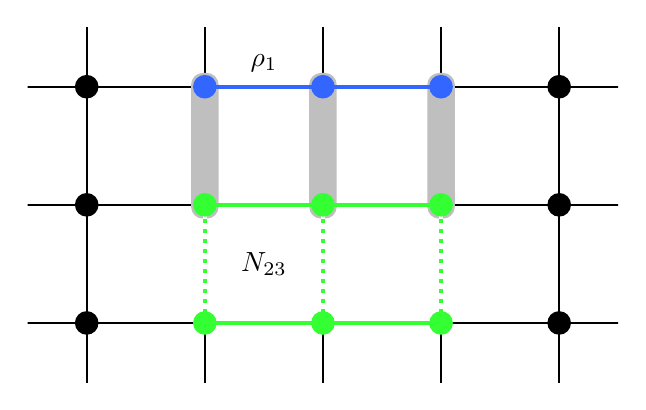
\begin{tikzpicture}[scale=0.5]
    % Define custom colors
\definecolor{customBlue}{rgb}{0.2, 0.4, 1}
\definecolor{customGreen}{rgb}{0.2, 1, 0.2}
\begin{scope}
\clip (-4.5,-1.5) rectangle (10.5,7.5);
\begin{scope}
    \foreach \x in {-6,-3,...,12} {
        \draw[thick, black] (\x,-3) -- (\x,9);
    }
    \foreach \y in {-3,0,...,9} {
        \draw[thick,black] (-6,\y) -- (12,\y);
    }
\end{scope}

    \fill[lightgray, rounded corners=0.15cm] (0-0.35,3+0-0.35) rectangle (0+0.35,6+0+0.35);
    \fill[lightgray, rounded corners=0.15cm] (3-0.35,3+0-0.35) rectangle (3+0.35,6+0+0.35);
    \fill[lightgray, rounded corners=0.15cm] (6-0.35,3+0-0.35) rectangle (6+0.35,6+0+0.35);

    \draw[customGreen, ultra thick] (0,0) -- (3,0) -- (6,0);  
    \draw[customGreen, ultra thick] (0,3) -- (3,3) -- (6,3);
    \draw[customBlue, ultra thick] (0,6) -- (3,6) -- (6,6);
    \draw[white, ultra thick] (0,0) -- (0,3);
    \draw[white, ultra thick] (3,0) -- (3,3);
    \draw[white, ultra thick] (6,0) -- (6,3);
    \draw[customGreen, ultra thick, dotted] (0,0) -- (0,3);
    \draw[customGreen, ultra thick, dotted] (3,0) -- (3,3);
    \draw[customGreen, ultra thick, dotted] (6,0) -- (6,3);


    \fill[black] (-3,0) circle (0.3);
    \fill[black] (-3,3) circle (0.3);
    \fill[black] (-3,6) circle (0.3);

    \fill[black] (9,0) circle (0.3);
    \fill[black] (9,3) circle (0.3);
    \fill[black] (9,6) circle (0.3);


    \fill[customGreen] (0,0) circle (0.3);
    \fill[customGreen] (3,0) circle (0.3);
    \fill[customGreen] (6,0) circle (0.3);

    \fill[customGreen] (0,3) circle (0.3);
    \fill[customGreen] (3,3) circle (0.3);
    \fill[customGreen] (6,3) circle (0.3);

    \fill[customBlue] (0,6) circle (0.3);
    \fill[customBlue] (3,6) circle (0.3);
    \fill[customBlue] (6,6) circle (0.3);

    \node[fill=white, inner sep=0pt] at (1.5,1.5) {$N_{23}$};
    \node at (1.5,6.6) {$\rho_1$};
\end{scope}
\end{tikzpicture}
}
\caption{ A tripartite graph state can be detected by preparing a network state, Bell measurements, and a fixed measurement. Entangled states of arrayed qubits can be detected by state preparation and a fixed measurement. }
\label{fig:chain}
\end{figure}

\begin{figure}
\centering
\resizebox{0.7\linewidth}{!}{
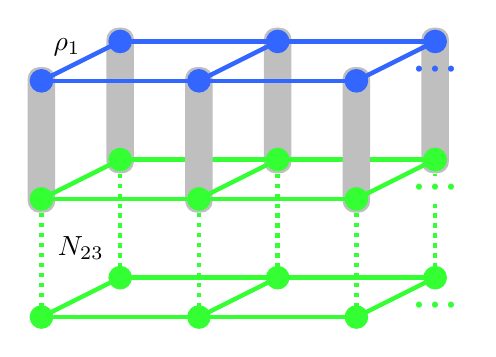
\begin{tikzpicture}[scale=0.5]
    % Define custom colors
    \definecolor{customBlue}{rgb}{0.2, 0.4, 1}
    \definecolor{customGreen}{rgb}{0.2, 1, 0.2}

    \fill[lightgray, rounded corners=0.15cm] (2-0.35,3+1-0.35) rectangle (2+0.35,6+1+0.35);
    \fill[lightgray, rounded corners=0.15cm] (6-0.35,3+1-0.35) rectangle (6+0.35,6+1+0.35);
    \fill[lightgray, rounded corners=0.15cm] (10-0.35,3+1-0.35) rectangle (10+0.35,6+1+0.35);

    \draw[customGreen, ultra thick] (0,0+0) -- (4,0+0) -- (8,0+0);  
    \draw[customGreen, ultra thick] (2,0+1) -- (6,0+1) -- (10,0+1); 
    \draw[customGreen, ultra thick] (0,0+0) -- (2,0+1);  
    \draw[customGreen, ultra thick] (4,0+0) -- (6,0+1);
    \draw[customGreen, ultra thick] (8,0+0) -- (10,0+1);

    \draw[customGreen, ultra thick] (2,3+1) -- (6,3+1) -- (10,3+1);

    \fill[lightgray, rounded corners=0.15cm] (0-0.35,3+0-0.35) rectangle (0+0.35,6+0+0.35);
    \fill[lightgray, rounded corners=0.15cm] (4-0.35,3+0-0.35) rectangle (4+0.35,6+0+0.35);
    \fill[lightgray, rounded corners=0.15cm] (8-0.35,3+0-0.35) rectangle (8+0.35,6+0+0.35);

    \draw[customGreen, ultra thick] (0,3+0) -- (4,3+0) -- (8,3+0);
    \draw[customGreen, ultra thick] (0,3+0) -- (2,3+1);
    \draw[customGreen, ultra thick] (4,3+0) -- (6,3+1);
    \draw[customGreen, ultra thick] (8,3+0) -- (10,3+1);
    
    \draw[customBlue, ultra thick] (0,6+0) -- (4,6+0) -- (8,6+0);
    \draw[customBlue, ultra thick] (2,6+1) -- (6,6+1) -- (10,6+1);
    \draw[customBlue, ultra thick] (0,6+0) -- (2,6+1);
    \draw[customBlue, ultra thick] (4,6+0) -- (6,6+1);
    \draw[customBlue, ultra thick] (8,6+0) -- (10,6+1);


    % First and second rows of disks
    \fill[customGreen] (0,0+0) circle (0.3);
    \fill[customGreen] (4,0+0) circle (0.3);
    \fill[customGreen] (8,0+0) circle (0.3);
    \fill[customGreen] (2,0+1) circle (0.3);
    \fill[customGreen] (6,0+1) circle (0.3);
    \fill[customGreen] (10,0+1) circle (0.3);

    \fill[customGreen] (0,3+0) circle (0.3);
    \fill[customGreen] (4,3+0) circle (0.3);
    \fill[customGreen] (8,3+0) circle (0.3);
    \fill[customGreen] (2,3+1) circle (0.3);
    \fill[customGreen] (6,3+1) circle (0.3);
    \fill[customGreen] (10,3+1) circle (0.3);

    \fill[customBlue] (0,6+0) circle (0.3);
    \fill[customBlue] (4,6+0) circle (0.3);
    \fill[customBlue] (8,6+0) circle (0.3);
    \fill[customBlue] (2,6+1) circle (0.3);
    \fill[customBlue] (6,6+1) circle (0.3);
    \fill[customBlue] (10,6+1) circle (0.3);

    \draw[customGreen, ultra thick, dotted] (0,0+0) -- (0,3+0);
    \draw[customGreen, ultra thick, dotted] (4,0+0) -- (4,3+0);
    \draw[customGreen, ultra thick, dotted] (8,0+0) -- (8,3+0);
    \draw[customGreen, ultra thick, dotted] (2,0+1) -- (2,3+1);
    \draw[customGreen, ultra thick, dotted] (6,0+1) -- (6,3+1);
    \draw[customGreen, ultra thick, dotted] (10,0+1) -- (10,3+1);

    \node at (10,0+0.25) [text=customGreen] {\huge \(\cdot\)\(\cdot\)\(\cdot\)};
    \node[fill=white, inner sep=0pt] at (10,3+0.25) [text=customGreen] {\huge \(\cdot\)\(\cdot\)\(\cdot\)};
    \node at (10,6+0.25) [text=customBlue] {\huge \(\cdot\)\(\cdot\)\(\cdot\)};

    \node[fill=white, inner sep=0pt] at (1,1.75) {$N_{23}$};
    \node at (0.65,6.85) {$\rho_1$};
\end{tikzpicture}
}
\caption{The estimation of entanglement witnesses for multipartite graph states.}
\label{graph state scheme}
\end{figure}

\subsection{ EWs for multipartite systems}

Thirdly, entanglement detection by state preparation can be extended to multipartite quantum states. We here, in particular, consider graph states, a class of states as a resource for MBQC \cite{PhysRevLett.86.5188}. Let us again present an instance for a three-qubit graph state, a Greenberger–Horne–Zeilinger (GHZ) state $|\psi\rangle = (|000\rangle +|111\rangle)/\sqrt{2}$ \cite{PhysRevA.62.062314}, see Fig. \ref{fig:chain}. An EW to detect a GHZ state may be given as,
\bea
W = \frac{1}{2} \mathbbm{1} - |\psi \rangle \langle \psi|.
\eea
A network state for an EW above can be constructed as,
\bea
N_{23} = \frac{1}{8} \sum_{a,b,c=0}^{1} \psi_{abc}^{(A_2 B_2 C_2)} \otimes \psi_{abc}^{(A_3 B_3 C_3)}.
\eea
where $\psi_{abc} = |\psi_{abc}\rangle \langle \psi_{abc}|$,
\bea
|\psi_{abc}\rangle = Z^a \otimes X^b \otimes X^c |\psi\rangle, ~~a,b,c \in \{0,1\}
\eea
with Pauli matrices $X$ and $Z$. It holds that
%\bea
%\tr[\rho W] =  8 \tr[\rho_1\otimes N_{23} P_{12} \otimes (\frac{\mathbbm{1}}{2} - |\psi \rangle\langle \psi |)_{3}], \nonumber
%\eea
\bea
{}_{A_3B_3C_3} \langle \psi |\rho_1 \otimes N_{23} ~P^{(12)} |\psi \rangle_{A_3B_3C_3} = \frac{1}{16} - \frac{1}{8}\tr[\rho W], \nonumber
\eea
which shows detection of a genuinely multipartite entangled state $\rho$ by finding that the left-hand-side is greater than $1/16$. Further generalization for detecting entangled $n$-qubit graph states is provided in Appendix. \\


\subsection{ To construct non-decomposable EWs }


Finally, let us investigate two entangled states defined by an EW. One denotes an entangled state $\rho_1$ detected by an EW, and the other $N_{23}$ realizing an EW by its preparation; see also Eq. (\ref{eq:ewm}). The result in Ref. \cite{PhysRevLett.96.150501} shows that an EW detects a set of entangled states that can activate its network state. Since a pair of PPT states cannot activate each other, either the states $\rho_1$ or $N_{23}$ must be non-PPT. Hence, a network state $N_{23}$ to detect a PPT entangled state $\rho_1$ should be non-PPT. We thus conclude that multipartite non-PPT entangled states can construct non-decomposable EWs, which are then highly non-trivial.
{
Note that non-PPT states can construct both decomposable and nondecomposable EWs, as shown in the example of reduction EWs, see Eq. \eqref{reductionEW}.
}
\\

{ \section{Robustness}
\label{sec:robust}

The framework for detecting entangled states in the subsection \ref{sec:gc} contains elements, the preparation of a network state and a fixed measurement for estimating a singlet fraction. We reiterate the relation between the estimation of an EW and the framework with a network state, 
\begin{align}
\tr[\rho W] = \alpha ~ \tr[\rho_1 \otimes N_{23} P^{(12)} (\eta \I - |\phi_{d}^+\rangle \langle \phi_{d}^+ | )_3 ],
\end{align}
for some $\alpha>0$. We here investigate the effect of noise on the preparation of a network state and a fixed measurement and show that the framework can unambiguously detect entangled states. That is, for separable states, the framework with noisy resources gives a non-negative expectation value. 


\begin{figure*}[t]
    \centering
    \includegraphics[scale=.18]{ fig4.pdf}
    \caption{  {Estimation of an EW in Eq. (\ref{eq:ewex}) can be realized in a circuit, where a network state in Eq. (\ref{eq:wr}) is realized and measurements in the computational basis are applied, see also Eq. (\ref{eq:ewr}). (1) A state for detecting entanglement, $|\psi^{-}\rangle$, is generated in registers $A_1B_1$. (2) A network state from an EW  is prepared to detect entanglement generated in $A_1B_1$. (3) A projection onto a state $|\phi^+\rangle $ is realized by collecting outcomes $00$ in registers $A_1A_2$. (4) A projection onto a state $|\phi^+\rangle $ is realized by collecting outcomes $00$ in registers $B_1B_2$. (5) Given outcomes $0000$ in registers $A_1B_1A_2B_2$, the singlet fraction is estimated in $A_3B_3$: a state in register $A_1B_1$ is entangled if the probability of outcomes $00$ in $A_3B_3$ is larger than $1/2$.  }}
    \label{fig:4}
\end{figure*}


\subsubsection*{ Noisy network states }
Suppose that the network states $N$ is noisy such that
\begin{align*}
\widetilde N &= (1-p) N + p \frac{\I}{d^{2n}},
\end{align*}
with some noise fraction $p$. It follows that,
\bea
&&\alpha~ \tr[\rho_1 \otimes \widetilde N_{23} P^{(12)} (\eta \I -  |\phi_{d}^+\rangle \langle \phi_{d}^+ | )_3 ] \nonumber \\
%&=&  \tr[\rho_1 \otimes ((1-p) N + p \frac{\I}{d^{2n}})_{23} P^{(12)} (\eta \I - \psi)_3 ]  \nonumber \\
&=& (1-p) \tr[\rho W] + \alpha p \frac{1}{d^{2n}} \frac{1}{d^{n}} (\eta d^n-1) \nonumber \\
&\geq & (1-p) \tr[\rho W]. \nonumber
\eea
Note that the term apart from $\tr[\rho W]$ in the second line is not negative since $\eta\leq 1/d$. Hence, noisy network states can be used to detect entangled states unambiguously. 



\subsubsection*{White noise in singlet fraction estimation}
Suppose that a fixed measurement setting for estimating a singlet fraction is noisy,
\begin{align}
(1-q)  |\phi_{d}^+\rangle \langle \phi_{d}^+ | + q \frac{\I}{d^n} \nonumber
\end{align}
with some noise fraction $q$. It follows that
\bea
&& \alpha ~ \tr[\rho_1 \otimes N_{23} P^{(12)} (\eta \I - (1-q)  |\phi_{d}^+\rangle \langle \phi_{d}^+ | - q \frac{\I}{d^n}  )_3 ]  \nonumber \\
 &= & (1-q)\tr[\rho W] + \alpha q \frac{1}{d^n} (\eta - \frac{1}{d^n} \tr[\rho^T N] ) \nonumber \\
 &\geq & (1-q) \tr[\rho W]. \nonumber
\eea
Thus, when a fixed measurement setting is noisy, the framework gives non-negative expectation values for separable states.

% \subsection{White noise in local Bell measurements}
% Now suppose that the local Bell measurements $P_{00}$ are replaced by  
% \begin{align*}
% \widetilde P = (1-r) P_{00} + r \frac{\I}{2^2}, % \label{noisy P}
% \end{align*}
% with the noise fraction $r$.
% With the noisy local Bell measurements, the state of interest $\rho$ is detected by MBEW if
% \begin{align}
% 0 &> \tr[\rho_1 \otimes N_{23} (\widetilde{P}\power{n})_{12} \otimes (\frac{1}{2}\I - \dyad{\vo}_G)^{(S'')}] \lb
% &= \tr \bigg[\rho_1 \otimes N_{23} (\frac{1}{2}\I - \dyad{\vo}_G)^{(S'')} \otimes \lb
% &\phantom{= \tr \bigg[} \left( \sum_{k=0}^{n} \binom{n}{k} q^{n-k} (\frac{1-q}{2^2})^k P_{00}\power{n-k} \otimes \I\power{k} \right)^{(SS')} \bigg] \lb
% &= \frac{1}{2^n} \tr \bigg[\rho_1 \otimes (\frac{1}{2}\I - \dyad{\vo}_G)^{(S')} \lb
% & \phantom{= \frac{1}{2^n} \tr\bigg[} \left( \sum_{k=0}^{n} \binom{n}{k} q^{n-k} (\frac{1-q}{2^2})^k P_{00}\power{n-k} \otimes \I\power{k} \right)^{(SS')} \bigg] \label{Bell noise exact}
% \end{align}
% It is too complicated to calculate exact value of the expression in the Ineq. (\ref{Bell noise exact}). Instead, let us consider an upper bound of the expression given by the worst case: the measurements are $P_{00}\power{n}$  (success) with a probability $q^n$, and $(\frac{\I}{2^2})\power n$ (fail) with a probability $1-q^n$. Then, the state $\rho$ is detected when
% \begin{align}
% \frac{1}{2^n} \left( q^n \frac{1}{2^n} \tr[\rho W] + (1-q^n) \frac{1}{2^{2n}} (\frac{1}{2} 2^n -1) \right) < 0,
% \end{align}
% which implies 
% \begin{align}
% \tr[\rho W] < (\frac{1}{2} - \frac{1}{2^n}) (1 - \frac{1}{q^n}).
% \end{align}
% }


\section{Realization in quantum circuits}


The framework of detecting entangled states by a fixed measurement can be realized in a quantum circuit. Here, we demonstrate the realization of a network state and the estimation of an EW with an example in Eq. (\ref{eq:ewex}). To facilitate the construction of a quantum circuit, we exploit a decomposition of the network state in the following, 
\begin{align}
N_{23} &= \frac{1}{4} \big( \ketbra{\psi^-}_{A_2 B_2} \otimes \ketbra{\phi^+}_{A_3 B_3}  \nonumber \\
&~~~~~~ + \ketbra{\psi^+}_{A_2 B_2} \otimes \ketbra{\psi^+}_{A_3 B_3} \nonumber \\
&~~~~~~ + \ketbra{\phi^-}_{A_2 B_2} \otimes \ketbra{\phi^-}_{A_3 B_3} \nonumber \\
&~~~~~~ + \ketbra{\phi^+}_{A_2 B_2} \otimes \ketbra{\psi-}_{A_3 B_3} \big), 
\end{align}
which is identical to the state in Eq. \eqref{eq:wr}. Then, a circuit for realizing the network state is shown in Fig. \ref{fig:4}, where blocks (1)-(5) describe realizations of a network state, projection on a state $|\phi^+\rangle$, measurements of estimating the singlet fraction. We remark that a fixed measurement setting is used for estimating an EW. 

Considering the effect of noise in Section \ref{sec:robust}, one may expect that the framework can be realized in a noisy implementation of quantum information processing. We then implemented the circuit in the IBMQ Kyiv on April 2, 2025. The results are presented in Fig. \ref{fig:result}, demonstrating the robustness of the proposed framework for estimating EWs in a realistic setting. Although noise is present, the estimation of an EW shows a singlet fraction $0.61$ higher than the threshold $1/2$, detecting the presence of an entangled state in registers $A_1B_1$.


%\begin{figure}[t]
%\centering
%\[
%\Qcircuit @C=1em @R=.7em @!R {
%\lstick{A_1} & \gate{H} & \ctrl{1} & \gate{Z} & \qw        & \qw        & \ctrl{2} & \gate{H} & \qw      & \qw      & \meter & \cw \\
%\lstick{B_1} & \qw      & \targ    & \gate{X} & \qw        & \qw        & \qw      & \qw      & \ctrl{2} & \gate{H} & \meter & \cw \\
%\lstick{A_2} & \gate{H} & \ctrl{1} & \gate{Z} & \qw        & \qw        & \targ    & \qw      & \qw      & \qw      & \meter & \cw \\
%\lstick{B_2} & \qw      & \targ    & \gate{X} & \targ      & \ctrl{0}   & \qw      & \qw      & \targ    & \qw      & \meter & \cw \\
%\lstick{A_3} & \gate{H} & \qw      & \qw      & \ctrl{-1}  & \qw        & \gate{H} & \ctrl{1} & \ctrl{1} & \gate{H} & \meter & \cw \\
%\lstick{B_3} & \gate{H} & \qw      & \qw      & \qw        & \ctrl{-2}  & \qw      & \targ    & \targ    & \qw      & \meter & \cw \\
%}
%\]
%    \caption{ The quantum circuit for detection of $\ket{\psi^-}_{A_1 B_1}$ using a pure network state $\ket{N}_{A_2B_2A_3B_3}$, which implements the EW $W = \tfrac{1}{2} \I - \psi^-$ \eqref{eq:ewex}. The first three layers in $A_1 B_1$ generate $\ket{\psi^-}$ state, while first five layers within $A_2 B_2 A_3 B_3$ generate $N$. The CNOT gates followed by $H$ gate and measurements in $A_1 A_2$ and $B_1 B_2$ implements local Bell projections. The measuremnet outcome $0000$ for the first four bits corresponds to the $\phi^+$ projections on both sides.}
 %   \label{fig:flip EW circuit}
%\end{figure}

\begin{figure}[t]
    \centering
    \includegraphics[scale=.13]{ fig5.pdf}
    \caption{ { The circuit in \ref{fig:4} is run in the IBMQ Kyiv. Given outcomes $0000$ in registers $A_1A_2B_1B_2$, the singlet fraction in registers $A_3B_3$ corresponds to the probability of having an outcome $00$. While $10000$ counts are obtained for registers $A_1A_2A_3B_1B_2B_3$, we have $685$ counts for $0000$ on $A_1A_2B_1B_2$, given which we have the singlet fraction $0.61$ which is larger than $1/2$. While the IBMQ Kyiv is noisy, we have demonstrated the generation and the detection of entangled states on a quantum circuit. 
    }}
    \label{fig:result}
\end{figure}

\section{Conclusion}


In conclusion, we have established an MB framework for estimating observables, in particular EWs, and shown the construction of network states for observables. It is also of fundamental interest to find that entanglement demonstrates elements of quantum theory, both dynamics, i.e., MBQC and observables. Our results shed new light on detecting and manipulating entangled states in a realistic scenario where precise controls via quantum gates are yet limited, such as an array of superconducting qubits, neutral atoms, or photons, where the preparation of a multipartite state and a fixed measurement are readily experimentally feasible. The results also open a new avenue of exploiting entangled states in distributed quantum information processing such as computing and metrology where entanglement is resourceful and quantum estimation {\it per se} corresponds to computing or metrology. 

In future directions, it would be interesting to realize the estimation of EWs via network states experimentally by considering the effects of noise in a realistic setting. Note that some network states, such as Smolin, have been realized in experiment \cite{Amselem:2009aa, PhysRevLett.105.130501, PhysRevLett.109.040501}. It is also interesting to exploit network states in a network and security scenario such as a measurement-device-independent scenario, see Refs. \cite{PhysRevLett.108.200401,PhysRevLett.110.060405}, so that observables such as EWs are estimated by relaxing assumptions on joint measurements; estimation of EWs, as well as detection of entanglement, is achieved in a higher level of robustness against imperfect implementations. 

\section*{Acknowledgement}

This work is supported by National Research Foundation of Korea (NRF-2021R1A2C2006309, NRF-2022M1A3C2069728) and the Institute for Information \& Communication Technology Promotion (IITP) (RS-2023-00229524, the ITRC Program/IITP-2023-2018-0-01402). AB and DC were supported by the Polish National Science Center project No. 2018/30/A/ST2/00837.


\bibliographystyle{quantum}
% \bibliography{bibedsp}
% \documentclass[a4paper,twocolumn,11pt,accepted=2017-05-09]{quantumarticle}
\documentclass[a4paper,twocolumn,10pt]{quantumarticle}
\pdfoutput=1
\usepackage[utf8]{inputenc}
\usepackage[english]{babel}
\usepackage[T1]{fontenc}
\usepackage{amsmath}
\usepackage{hyperref}

\usepackage{tikz}
\usepackage{lipsum}

\newtheorem{theorem}{Theorem}


\usepackage{tikz}
\usepackage{qcircuit}
%%%%%%%%%%%%%%%%%%

%\usepackage{IEEEtrantools}
\usepackage{multirow}

% ------------------------------------------------------------------------------
\newcommand{\rev}{\color{blue}}
\newcommand{\bae}{\color{purple}}
\newcommand{\ji}{\color{gray}}

\newcommand{\vx}{\Vec{x}}
\newcommand{\vy}{\Vec{y}}
\newcommand{\vo}{\Vec{0}}
\newcommand{\Va}{\Vec{a}}
\newcommand{\Vb}{\Vec{b}}
\newcommand{\power}[1]{^{\otimes #1}}
\newcommand{\lb}{\nonumber \\}


\newcommand{\R}{\mathbb{R}}
\newcommand{\N}{\mathbb{N}}
\newcommand{\C}{\mathbb{C}}
\newcommand{\Z}{\mathbb{Z}}
\newcommand{\Q}{\mathbb{Q}}
\newcommand{\I}{\mathbbm{1}}

\newcommand{\tr}{\text{tr}}
\newcommand{\ket}[1]{| #1 \rangle}
\newcommand{\bra}[1]{\langle #1|}
\newcommand{\ip}[2]{\langle #1|#2 \rangle}
\newcommand{\bracket}[3]{\langle #1|#2|#3 \rangle}
\newcommand{\sm}[1]{\left( \begin{smallmatrix} #1 \end{smallmatrix} \right)}

\newcommand{\be}{\begin{equation}}
\newcommand{\ee}{\end{equation}}
\newcommand{\bea}{\begin{eqnarray}}
\newcommand{\eea}{\end{eqnarray}}
\newcommand{\bes}{\begin{equation*}}
\newcommand{\ees}{\end{equation*}}
\newcommand{\beas}{\begin{eqnarray*}}
\newcommand{\eeas}{\end{eqnarray*}}

% ------------------------------------------------------------------------------

\newcommand{\x}{\mathrm{x}}
%\newcommand{\ket}[1]{|#1\rangle}
\newcommand{\ketbra}[1]{\ket{#1}\!\bra{#1}}
%\newcommand{\bra}[1]{\langle#1|}
\newcommand{\dyad}[1]{\ket{#1}\!\bra{#1}}

\newcommand{\ten}{\otimes}
\newcommand{\Id}{\mathds{1}}
\newcommand{\zero}{\mathbf{0}}
\newcommand{\KBDS}{C^{s}}
\newcommand{\KBDSs}{C}
%\newcommand{\KBDS}{C^{\mbox{\tiny U}}}
\newcommand{\KTwo}{C^{2\times2}}
\renewcommand{\H}{\mathcal{H}}
\def\A{\mathcal{A}}
\def\B{\mathcal{B}}

\def\x{\mathrm{x}}
\def\y{\mathrm{y}}

\def\W{\mathcal{W}}


\def\sig{\widetilde{\sigma}}
\def\F{\mathcal{F}}
\def\N{\mathcal{N}}
\def\P{\mathbbm{P}}
\def\tr{\mathrm{tr}}

\def\L{\mathcal{L}}
\def\Q{\mathcal{Q}}
\def\NL{\mathcal{NS}}

\DeclareMathOperator*{\Oplus}{\bigoplus}
\DeclareMathOperator*{\Otimes}{\bigotimes}
% \DeclareMathOperator*{\Oplus}{\scalerel*{\bigoplus}{\textstyle\sum}}
% ------------------------------------------------------------------------------






\begin{document}

\title{ Detecting Entanglement by State Preparation and Local Measurements}


\author{Jaemin Kim}
\email{woals6584@kaist.ac.kr}
\affiliation{School of Electrical Engineering, Korea Advanced Institute of Science and Technology (KAIST), 291 Daehak-ro, Yuseong-gu, Daejeon 34141, Republic of Korea }
\orcid{ }


\author{Anindita Bera}
\email{aninditatitli@gmail.com}
\affiliation{Department of Mathematics, Birla Institute of Technology Mesra, Jharkhand 835215, India}
\orcid{ }


\author{Dariusz Chru\'sci\'nski}
\email{darch@fizyka.umk.pl}
\affiliation{Institute of Physics, Faculty of Physics, Astronomy, and Informatics, Nicolaus Copernicus University, Grudziadzka 5, 87-100 Torun, Poland}
\orcid{ }

\author{Joonwoo Bae}
\email{joonwoo.bae@kaist.ac.kr}
\affiliation{School of Electrical Engineering, Korea Advanced Institute of Science and Technology (KAIST), 291 Daehak-ro, Yuseong-gu, Daejeon 34141, Republic of Korea }
\orcid{ }


\maketitle

\begin{abstract}
  Entanglement witnesses (EWs) are a collection of observables that can characterize separable states and, experimentally, estimating EWs can verify entangled states. In this work, we show that a fixed measurement setting on a multipartite entangled state, which we introduce as a \emph{network state} for the purpose, can estimate EWs. Namely, entangled states can be fully verified in a measurement-based manner, in which experimenters do not necessarily change measurement settings. We present a fixed measurement setting and network states for estimating decomposable EWs, equivalent to the partial transpose criteria. We also consider non-decomposable EWs that detect bound entangled states beyond the partial transpose criteria. The results can be extended to multipartite states such as graph states, a resource for measurement-based quantum computing, and readily applied to distributed settings such as quantum metrology or sensor networks where multipartite entangled states are resourceful.
\end{abstract}





\section{Introduction}


{Entangled states are a key resource in quantum information processing, in particular, to achieve quantum advantages in computation and communication tasks. A higher level of security in cryptographic protocols \cite{PhysRevLett.98.230501}, higher level of quantum certification \cite{Pironio_2009, PhysRevLett.110.060405, PhysRevLett.108.200401, Bowles:2018aa} and higher network channel capacities \cite{PhysRevA.95.052329, PhysRevLett.125.150502} can be achieved by exploiting entangled states. Efficient computation with quantum resources can be realized by local measurements and entangled states only, called measurement-based quantum computation (MBQC) \cite{PhysRevLett.86.5188, MeasurementBasedQuantumComputation, Briegel:2009aa}. }

{ Entanglement witnesses (EWs) \cite{TERHAL2000319, PhysRevA.62.052310} are versatile tools to detect entangled states both theoretically and experimentally. They correspond to observables that are non-negative for all separable states but negative for some entangled states \cite{HORODECKI19961, GUHNE20091, RevModPhys.81.865, Chru_ci_ski_2014, Friis:2019aa}. Hence, negative expectation values of EWs unambiguously conclude the presence of entangled states. In practice, multiple measurement settings may be necessary for estimating EWs. }

{ In this work, we show that a fixed measurement setting can detect entangled states, together with the preparation of a multipartite state, which we call a {\it network state}. To be precise, we present a framework for detecting entangled states such that a fixed measurement over a network state $N$ and a state $\rho$ can find if the state $\rho$ is entangled, where a network state $N$ is obtained from an EW. Thus, entangled states can be verified in a measurement-based (MB) manner. In fact, the framework is closely connected to the activation of entanglement in that it finds if a state $\rho$ is entangled if a joint state $N\otimes \rho$ is more entangled than a state $N$. }

We show how network states can be obtained from EWs. We present the construction of network states for decomposable EWs, which are equivalent to the partial transpose criteria, and also for non-decomposable EWs that detect bound entangled states beyond the partial transpose criteria, such as the Bell-diagonal EWs \cite{chruscinski2014class, PhysRevA.105.052401} from the Choi map \cite{Choi:1975aa} and its various generalizations \cite{PhysRevA.84.024302}, and the Breuer-Hall EW \cite{PhysRevLett.97.080501, Hall_2006}. The results are extended to multipartite systems: graph states \cite{PhysRevA.69.062311}, a resource for MBQC \cite{PhysRevLett.86.5188}, can be detected by network states and a fixed measurement.
{ 
We discuss the connection of our work to the entanglement activation \cite{PhysRevLett.96.150501} and the measurement-device-independent entanglement witnesses \cite{PhysRevLett.110.060405}.
}

The importance of our results is threefold. Firstly, similarly to MBQC, one can circumvent the control of multiple measurement settings when estimating observables. Precise controls on and the preparation of general measurements identify additional difficulties for realizing EWs in general. Our results show that the preparation of quantum states and a fixed measurement can be an experimentally feasible alternative. Secondly, it is of fundamental interest to find that entangled states with a fixed measurement are a resource that can be replaced with observables. Note that MBQC signifies that entangled states and local measurements can be an alternative to realize quantum state transformation. Finally, the framework for estimating EWs in an MB manner finds various usefulness of distributed settings such as distributed quantum metrology over networks, e.g., \cite{Chabuda:2020aa, Zhang_2021,Len:2022aa, PhysRevLett.121.043604}: estimation of joint observables enables distributed quantum information processing, e.g., \cite{PhysRevA.85.062326, Friis_2017, PhysRevLett.120.080501}.

\section{Entanglement detection}
 
Let us begin by describing an experimental scenario of verifying entangled states, where the scenario is common in various experimental settings. We consider two quantum systems $A$ and $B$ on a Hilbert space $\H\otimes \H$. Interestingly, observables exist, denoted by $W=W^{\dagger}$, such that, for all separable states $\sigma_{\mathrm{sep}}$, 
\bea
\tr[W\sigma_{\mathrm{sep}}] \geq 0~~\mathrm{and }~~ \tr[W\rho_{\mathrm{ent}}] <0\nonumber
\eea
for some entangled states $\rho_{\mathrm{ent}}$ \cite{TERHAL2000319, PhysRevA.62.052310}. All entangled states can be verified by estimating some observables, which are called entanglement witnesses (EWs). In experiment, EWs can be estimated by altering measurement settings in general: negative expectation values unambiguously conclude entangled states \cite{GUHNE20091}. They can be also used to verify other properties, other than entanglement, such as a fidelity in the state preparation \cite{PhysRevA.76.030305, Haffner:2005aa}.

%Note that the structure of EWs remains } 


%One of the intriguing properties of entangled states is the irreversibility in manipulations of entanglement. Entangled states from which no entanglement can be extracted, though entanglement is needed for their preparation, are identified as {\it undistillable} or {\it bound} entangled states \cite{PhysRevA.61.062313, PhysRevLett.86.2681}. Multipartite quantum states that remain positive after partial transpose (PPT) turn out to be undistillable. Remarkably, PPT entangled states can be used to activate other entangled states \cite{horodecki1999bound}.

%Then, non-PPT entangled states can be characterized by decomposable EWs that have a general form as follows,
%\bea
%W = P+Q^{\Gamma},~~\mathrm{for}~~P,~Q\geq 0\nonumber.
%\eea
%Here $\Gamma$ denotes the partial transpose. Then, non-decomposable EWs, which cannot be in the form above, can detect PPT entangled states. 

%\cite{PhysRevA.61.062313, PhysRevLett.86.2681}.

%In general, it is highly non-trivial to construct non-decomposable EWs, which are the main object in the mathematically challenging problem of classifying positive linear maps of Operator Algebras \cite{Stormer:1963aa}, see also Refs. \cite{bera2022generalizing, bera2022class,mirror}.

{\section{Measurement-Based Estimation}

Let us show that observables can be generally estimated in a measurement-based manner. We here focus on EWs, observables of particular interest for detecting entangled states, and provide the scheme for estimating of single observables in Appendix. We devise multipartite quantum states, {\it called network states}, for estimating observables. 

\subsection{Example }
\label{subsec:ex}
Let us begin with an illuminating example of an MB estimation of an EW. Throughout, Bell states are denoted by $|\phi^{\pm}\rangle = (|00\rangle \pm |11\rangle)/\sqrt{2}$ and $|\psi^{\pm}\rangle = (|01\rangle \pm |10\rangle)/\sqrt{2}$. We consider an EW in the following,
\bea
%W = \frac{1}{2} \mathbbm{1} - |\psi^{-} \rangle \langle \psi^{-} |, \nonumber
W = \frac{1}{4} (\mathbbm{1} + X\otimes X + Y\otimes Y + Z\otimes Z) \label{eq:ewex}
\eea
where $X,Y$ and $Z$ are Pauli matrices. Eq. (\ref{eq:ewex}) shows that an EW can be estimated by various measurement settings. Note that a Bell state $|\psi^{-}\rangle$ is detected by an EW above. 
 
 
%\subsection{Two-qubit network states}

The MB framework for estimating an observable in Eq. (\ref{eq:ewex}) can be achieved by a four-partite state, called a {\it network state}, constructed as follows, 
\bea
N_{23} &=& \frac{1}{4} |\psi^-\rangle_{A_2B_2} \langle \psi^-| \otimes |\phi^+\rangle_{A_3B_3} \langle \phi^+| + \nonumber \\
&&\frac{1}{12} (\mathbbm{1} - |\psi^-\rangle_{A_2B_2} \langle \psi^-|) \otimes (\mathbbm{1} - |\phi^+\rangle_{A_3B_3} \langle \phi^+|),~~~~ ~\label{eq:wr}
\eea

on sites $A_2A_3B_2B_3$, see Fig. \ref{fig:fig1}. We then place a state of interest at $A_1B_1$, denoted by $\rho_{1}:=\rho^{( A_1B_1)}$, which we want to learn if it is entangled. We have
\bea
\tr[\rho W ] =  16~ \tr  [\rho_1\otimes N_{23} (\frac{1}{2}\mathbbm{1} - | \phi^+\rangle_{A_3B_3} \langle \phi^+|) \otimes P^{(12)}],~~
\label{eq:ewr}
\eea
where $P^{(12 )} = |\phi^{+}\rangle_{A_1A_2}\langle \phi^+| \otimes |\phi^{+}\rangle_{B_1B_2}\langle \phi^+|$. Eq. (\ref{eq:ewr}) can be simplified by a singlet fraction as follows,
\bea
_{A_3 B_3}  \langle \phi^{+}| \tr_{12}[ \rho_1 \otimes N_{23} ~P^{(12)} ]  |\phi^{+}\rangle_{A_3 B_3}   = \frac{1}{8} - \frac{1}{4}\tr[\rho W].~~
\label{eq:expew}
\eea
The left-hand-side can be obtained by preparing a network state followed by a fixed measurement. A state $\rho_1$ is entangled if the right-hand-side is greater than $1/8$ since $\tr[\sigma_{\mathrm{sep}}W ]\geq 0 $ for all separable states $\sigma_{\mathrm{sep}}$. Once a Bell measurement reports an outcome $P^{(12)} $, a singlet fraction is estimated from the probability of having outcome $|\phi^{+}\rangle$ on $A_3B_3$. Thus, it is shown that an EW can be estimated in a fully MB manner. 

%In fact, an entangled state $\rho$ is detected if the probability, i.e., the left-hand-side in Eq. (\ref{eq:expew}), is greater than $1/8$, since $\tr[\sigma_{\mathrm{sep}}W ]\geq 0 $ for all separable states $\sigma_{\mathrm{sep}}$.


Experimental resources to realize the MB framework, i.e., the left-hand side in Eq. (\ref{eq:expew}), are as follows. A network state is required, see Eq. (\ref{eq:ewex}), which is entangled and bi-separable. The detection scheme needs a measurement in the basis $|\phi^+\rangle$, which is equivalent to the capability of realizing a controlled-NOT gate, a Hadamard gate, and a fixed-measurement in the $z$-direction; see also Fig. \ref{fig:fig1}. All these are compatible with the resources to realize MBQC. In addition, it is worth mentioning that a network state in Eq. (\ref{eq:wr}) is a variation of a Smolin state, a four-partite bound entangled state \cite{PhysRevA.63.032306}, which has been repeatedly realized in experiment \cite{ Amselem:2009aa, PhysRevLett.105.130501, PhysRevLett.109.040501}. It should be pointed out that a realization of the presented MB framework is readily available in an experiment. 



\begin{figure}[t]
\centering
% \includegraphics[width=9.0cm ]{figure1}
\resizebox{0.9\linewidth}{!}{
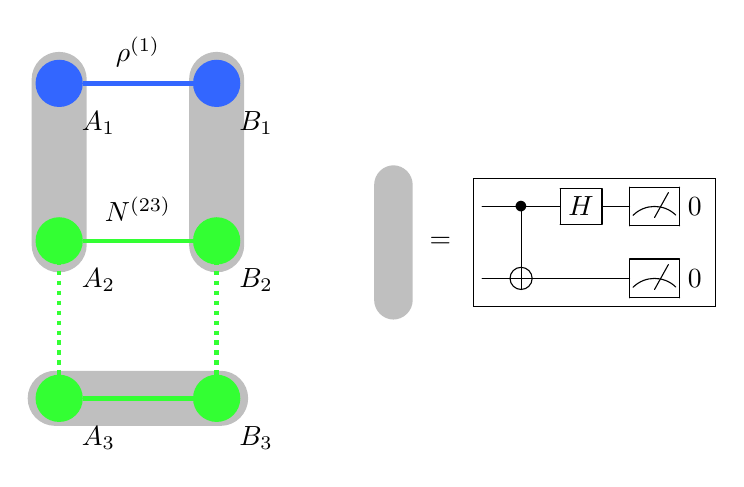
\begin{tikzpicture}[scale=2]
    % Define custom colors
    \definecolor{customBlue}{rgb}{0.2, 0.4, 1}
    \definecolor{customGreen}{rgb}{0.2, 1, 0.2}

    % Round-edged rectangles and dotted lines for both rows
\fill[lightgray, rounded corners=0.35cm] (-0.175,1.2) rectangle (0.175,-0.2);
\fill[lightgray, rounded corners=0.35cm] (-1-0.175,1.2) rectangle (-1+0.175,-0.2);
\fill[lightgray, rounded corners=0.35cm] (-0.5-0.7,-0.825) rectangle (-0.5+0.7,-1.175);
\draw[customGreen, ultra thick, dotted] (0,0) -- (0,-1);
\draw[customGreen, ultra thick, dotted] (-1,0) -- (-1,-1);

% Green ultra thick lines between A2-B2 and A3-B3
\draw[customGreen, ultra thick] (0.15,0) -- (-1+0.15,0);
\draw[customGreen, ultra thick] (0.15,-1) -- (-1+0.15,-1);

% Blue ultra thick line between A1 and B1
\draw[customBlue, ultra thick] (0.15,1) -- (-1+0.15,1);

    % First row of disks
    \fill[customBlue] (0,1) circle (0.15);
    \fill[customGreen] (0,0) circle (0.15);
    \fill[customGreen] (0,-1) circle (0.15);

    % Second row of disks
    \fill[customBlue] (-1,1) circle (0.15);
    \fill[customGreen] (-1,0) circle (0.15);
    \fill[customGreen] (-1,-1) circle (0.15);

    % Captions
    \node at (-0.5,1.2) {$\rho^{(1)}$};
    \node at (-0.5,0.2) {$N^{(23)}$};

% Labels
\node at (-1+0.25,0.75) {$A_1$};
\node at (-1+0.25,-0.25) {$A_2$};
\node at (-1+0.25,-1.25) {$A_3$};
\node at (+0.25,0.75) {$B_1$};
\node at (+0.25,-0.25) {$B_2$};
\node at (+0.25,-1.25) {$B_3$};

    \begin{scope}[xshift=1cm, yshift=-0.5cm, scale=0.7] % Adjust yshift for spacing between figures
        \fill[lightgray, rounded corners=0.25cm] (0,0) rectangle (0.35,1.4);

        \node at (0.6,0.7) {$=$};

        % Quantum Circuit inside a TikZ node
        \node[draw, inner sep=3pt] at (2,0.7) {
            \Qcircuit @C=1em @R=1.2em {
            % Qubit setup
            \lstick{} & \ctrl{1} & \gate{H} & \meter & \rstick{\hspace{-1.2em} 0} \\
            \lstick{} & \targ    & \qw      & \meter & \rstick{\hspace{-1.2em} 0} \\
            }
        };
    \end{scope}
\end{tikzpicture}
}
\caption{ A four-partite network state $N_{23}$ is prepared on $A_2A_3B_2B_3$ to detect an entangled state on $A_1B_1$. Bi-interactions and measurements in the computational basis can construct EWs, see also Eq. (\ref{eq:expew}) in the text. Gray boxes denote a measurement in the basis $|\phi^{+}\rangle$, which is equivalent to a measurement in the computational basis after applying of a controlled-NOT gate followed by a Hadamard gate. }
\label{fig:fig1}
\end{figure}



\subsection{ EWs via entanglement activation}

To show a general construction of network states for arbitrary EWs for high-dimensional quantum systems, we want to clarify their relations to activation of entanglement \cite{PhysRevLett.96.150501}: all EWs can be expressed in the following form, }
\bea
W_{A_2 B_2 } = \tr_{A_3B_3} \big[N (\eta \mathbbm{I} - |\phi_{d}^+ \rangle_{A_3B_3} \langle \phi_{d}^+ |)\big], \label{eq:ewm}
\eea
for some network state $N := N^{(A_2 B_2 A_3 B_3)}$ and a parameter $\eta \in [1/d,1 )$, where $|\phi_{d}^+\rangle = \sum_{j=0}^{d-1}|jj\rangle /\sqrt{d}$. It is worth mentioning an EW above shares similarity with Eq. (\ref{eq:ewr}) Note that the parameter $\eta$ satisfies the condition, $\eta\geq E_d [N]$ where $E_d$ is called a maximal singlet fraction,
\bea
E_d[N] &=& \sup_{\F}~ \langle \phi_{d}^+| \F[ N ] |\phi_{d}^+\rangle ~\mathrm{for~a~local ~filtering~}\F   \nonumber \\
&& \F[N] = \frac{ K_{A}\otimes K_B N K_{A}^{\dagger}\otimes K_{B}^{\dagger} }{ \tr[  K_{A}^{\dagger}K_{A} \otimes K_{B}^{\dagger}K_{B} N ]},\label{eq:fil}
\eea
where $K_A: \H_{A_1A_2}\rightarrow \mathbbm{C}^d $ and $K_B: \H_{B_1B_2}\rightarrow \mathbbm{C}^d $. It is worth mentioning that EWs in Eq. (\ref{eq:ewm}) identify entangled states that activate a network state in the sense that
\bea
E_d[ \sigma\otimes N]>\eta, ~\mathrm{whereas}~ {E_d [N]\leq \eta}.\label{eq:ac}
\eea
In fact, all entangled states can be used to activate some other state: in Eq. (\ref{eq:ac}) a state $\sigma$ is entangled if and only if it can activate some other entangled state $N$.



{ 
\subsection{ Detection protocol from  entanglement activation}

We exploit the scenario of activating entanglement as a framework for detecting entangled states. Namely, a state $\rho$ is entangled if it can be used to activate a state $N$. To this end, we consider a local filtering operation $\Phi$ as follows,
\begin{align}
\Phi (\rho \otimes N) = \tr_{A_1 B_1 A_2 B_2}[ P^{(12)} \rho^{(A_1 B_1)} \otimes N^{(A_2 B_2 A_3 B_3)}]. \nonumber
\end{align}
where $P^{(12)}$ the projection onto maximally entangled states as follows,
\bea
P^{(12 )} = |\phi_{d}^{+}\rangle_{A_1A_2}\langle \phi_{d}^+| \otimes |\phi_{d}^{+}\rangle_{B_1B_2}\langle \phi_{d}^+| \label{eq:projd} 
\eea
and $|\phi_{d}^+\rangle = \sum_{i=1}^d|ii\rangle/\sqrt{d}$. The singlet fraction after the filtering operation is given by,
\begin{align}
F_{\Phi}(\rho \otimes N) = \frac{ \bracket{\phi_d^+}{\Phi(\rho \otimes N)}{\phi_d^+} }{\tr[\Phi(\rho \otimes N)]}.\nonumber
\end{align}
With the specific local operation, the singlet fraction of a network state $N$ can be computed as, 
\begin{align}
\widetilde E_d(N) = \sup_{\sigma \in \mathrm{SEP}} F_{\Phi}(\sigma \otimes N),
\end{align}
where $\mathrm{SEP}$ denotes the set of separable states. It is clear that $\widetilde E_d(N) \le E_d(N)$ since a specific local operation is considered. Note also that for $\eta \in [\frac{1}{d},1)$, there exists a state $N$ such that $E_d(N) = \widetilde E_d(N) = \eta$ \cite{PhysRevLett.96.150501}. It holds that a state $\rho$ is entangled if we have $F_{\Phi}(\rho \otimes N) > \eta $ for $N$ such that $\widetilde E_d(N) \leq \eta$. 
}




\subsection{ General construction of network states }
\label{sec:gc}

Let us then present a construction of a network state for a given EW, see also Eq. (\ref{eq:ewm}). Suppose that an EW on $d\otimes d$ is decomposed as follows,
\bea
W = \sum_{j} a_j W(j)^T ~\mathrm{with}~ W(j) \geq 0 ~\mathrm{and}~ a_j \in \mathbbm{R}, \label{eq:eeww}
\eea
so that one can choose normalized non-negative operators $\{ \Pi(i) \geq 0\}$ and real constants $\{ c_j\}$ such that,
\bea
N_{23} &=&\sum_{j} c_j  W(j)_{A_2B_2} \otimes  \Pi(j)_{A_3B_3}, ~\mathrm{and}  \label{eq:ns} \\
W_2 & =& ~ k \, \tr_{3} [N_{23}^{T_2}  ( \eta \mathbbm{1} - |\phi_{d}^+ \rangle_{A_3B_3} \langle \phi_{d}^+ |  )  ], \label{eq:ewn}
\eea
for some $\eta\geq 1/d$ and $k>0$, where $W_2$ reproduces a given EW in Eq. (\ref{eq:eeww}) on sites $A_2 B_2$. One can find $\{a_j\}$ and $\{c_j \}$ are related as follow,
\bea
a_j = k \, c_j (\eta - \bracket{\phi_{d}^+}{\Pi(j)}{\phi_{d}^+}).\nonumber
\eea
Then, for a state $\rho_1 = \rho^{(A_1B_1)}$ it holds that
\bea
\tr[\rho W] %&=& d^2 ~ \tr[\rho_1 \otimes W_{2}^T P^{(12)}  ]  \nonumber\\
&\propto& \tr[\rho_1 \otimes N_{23} ~ P^{(12)} \otimes ( \eta \mathbbm{1} - |\phi_{d}^+ \rangle_{A_3B_3} \langle \phi_d^+ |  ) ]. ~~~~~ \label{eq:m}
\eea
For an entangled state $\rho$ detected by $W$, i.e., $\tr[\rho W]<0$, Eq. (\ref{eq:m}) shows that
\bea
\eta &<&  _{A_3B_3}\langle \phi_{d}^+| \Lambda^{(1\rightarrow 3)} [\rho_1]|\phi_{d}^+\rangle_{A_3B_3} \nonumber \\
&&\mathrm{where}~ \Lambda^{( 1\rightarrow 3)} [\rho_1]= \frac{ \tr_{12}[\rho_{1}\otimes N_{23} P^{(12)}] }{ \tr[\rho_1\otimes N_{23} P^{(12)}]  }. ~~\label{eq:v}
\eea
Note that the construction above applies to all EWs in general.\\

{
{\it Example.} A straightforward and facile construction of a network state from an EW is as follows. For an EW, we find a decoposition,
\bea
 W = a_+ W_+^T - a_- W_-^T\nonumber
 \eea
with coefficients $a_{\pm} > 0$ and quantum states $W_{\pm}$ (i.e., $W_{\pm} \ge 0$ and $\tr[W_{\pm}]=1$). We choose $\eta = 1/d$ and find a network state as follows,
\begin{align}
N_{23} &=c_+ W_+ \otimes \frac{\I-\dyad{\phi^+_d}}{d^2-1} +  c_- W_- \otimes \dyad{\phi^+_d}.\nonumber
\end{align}
where
\bea
c_+ = \frac{(d-1)a_+}{(d-1)a_+ + a_-} ~~\mathrm{and} ~~c_-= \frac{a_-}{(d-1)a_+ + a_-}. \nonumber
\eea 
We have presented a straightforward one by exploiting a spectral decomposition of an EW. We also stress that a network state is not unique for an EW. \\
}

A quantum teleportation protocol may rephrase Eq. (\ref{eq:v}) as follows. Once a measurement $P^{(12)}$ is successful, a state $\rho$ prepared at $A_1B_1$ is teleported at $A_3B_3$ via a network state $N_{23}$. Note that the map in Eq. (\ref{eq:v}) is a probabilistic operation assisted by entanglement \cite{PhysRevA.64.012317}; to be precise, successful Bell measurements define a channel for a state $\rho_1$ \cite{Jamiokowski:1972aa, Choi:1975aa}. Finally, a singlet fraction is estimated and compared with $\eta$, see Eq. (\ref{eq:v}), to verify entanglement. We have shown that, given an EW, one can always construct a network state for the estimation as above. 

As mentioned, experimental resources for the realization contain preparing a network state and Bell measurements that require bi-interactions and a fixed local measurement setting; see also Fig. \ref{fig:fig1}. In Appendix, we reproduce a network state in Eq. (\ref{eq:wr}) by applying the general construction above.

{
\subsection{ Noisy local projections on $A_1A_2$ and $B_1B_2$: semi measurement-device-independent entanglement witnesses } 
\label{semi MDI}

The framework of detecting entanglement relies on projections to maximally entangled states, see Eq. (\ref{eq:projd}). It bears some similarity with the measurement-device-independent (MDI) scenario \cite{PhysRevLett.108.200401,PhysRevLett.110.060405}, which applies when one wants to relax the assumption to trust measurement devices. Then, an MDI scenario trusts on state preparations and relaxes the assumptions on joint measurements. 

Similarly, we here show that projections on  $A_1A_2$ and $B_1B_2$, joint measurements performed locally, can be relaxed for the verification of entangled states. To this end, we show that untrusted joint measurements on $A_1A_2$ and $B_1B_2$ can unambiguously conclude entangled states. Let us consider a separable state $\sigma = \sum_k p_k \tau_k \otimes \xi_k$ and a threshold  $\eta$. Let $Q^{(A_1 A_2)}$ and $R^{(B_1B_2)}$ denote unknown positive-operator-valued-measure elements that may describe detection events of untrusted measurement devices. It suffices to show that $\sigma$ cannot increase the singlet fraction of $N$ larger than the threshold $\eta$. This means, 
\bea
\tr[(Q^{(A_1 A_2)} \otimes R^{(B_1 B_2)} \sigma_1 \otimes W_{2}^T]  \geq 0 \nonumber
\eea
for all $Q$ and $R$, see also $W_{2}^T$ in Eq. (\ref{eq:ewn}). We then have: 
\bea
&& \sum_k p_k \tr[(Q^{(A_1 A_2)} \otimes R^{(B_1 B_2)}) (\tau_k^{(A_1)} \otimes \xi_k^{(B_1)}) W_{2}^T ] \nonumber \\
%&=& \sum_k p_k \tr[(\widetilde{Q}^{(A_2)} \otimes \widetilde{R}^{(B_2)}) N_{23} (\eta \I - \dyad{\phi^+_d})_3] \nonumber \\
%&\propto \sum_k p_k \tr[(\widetilde{Q} \otimes \widetilde{R})_2 W^T_2] \nonumber\\
&\propto& \sum_k p_k \tr[(\widetilde{Q}^T \otimes \widetilde{R}^T) W] \ge 0 \nonumber 
\eea
since 
\begin{align*}
\widetilde{Q}^{(A_2)} &= \tr_{A_1}[Q^{(A_1 A_2)} (\sigma_k^{(A_1)} \otimes \I^{(A_2)})] \ge 0, \\
\widetilde{R}^{(B_2)} &= \tr_{B_1}[R^{(B_1 B_2)} (\xi_k^{(B_1)} \otimes \I^{(B_2)})] \ge 0\nonumber
\end{align*}
and an EW is non-negative for all separable states. Hence, we have shown that joint measurements on $A_1A_2$ and $B_1B_2$ with untrusted measurements can also unambiguously conclude entangled states. 
}

\section{Examples}


Let us apply the general construction of network states and present network states for EWs known so far, such as decomposable and non-decomposable instances, the latter of which are highly non-trivial in Quantum Information Theory. Identifying all EWs is equivalent to characterizing the set of separable states, which is a challenging mathematical problem \cite{Stormer:1963aa}; the computational complexity also belongs to NP-Hard \cite{10.1145/780542.780545}. The construction of network states applies to all EWs. In what follows, we apply the general construction of network states to non-trivial EWs.

To this end, let $P_{st}$ denote a projection onto a Bell state, for $s,t = 0,\ldots, d-1$, in a dimension $d$,
\bea
P_{st} = |\phi_{st}\rangle \langle \phi_{st}| ~\mathrm{where}~|\phi_{st} \rangle = \frac{1}{\sqrt{d}} \sum_{j = 0}^{d-1} \omega^{t j } \ket{j } \ket{j + s}, ~~ \label{eq:1}
\eea
where $\omega = e^{2\pi i/d}$.
Projectors onto symmetric and anti-symmetric subspaces are denoted by $S_d$ and $A_d$, respectively,
\bea
S_d = \frac{\mathbbm{1+F} }{2}~~\mathrm{and} ~~A_d = \frac{\mathbbm{1 - F} }{2},
\eea
where $\mathbbm{F} = d P_{00}^{\Gamma}$ is a flip operator and $\Gamma$ denotes the partial transpose \cite{PhysRevA.61.062313}. Note that $\tr[A_d]=d(d-1)/2$ and $\tr[S_d] = d(d+1)/2$. Interestingly, high-dimensional Bell states and projections onto symmetric and anti-symmetric subspaces suffice to construct network states for known non-decomposable maps.



\subsection{ Decomposable EWs: the partial transposition }

Firstly, we consider a decomposable EW $W = Q^\Gamma$ for $Q\geq 0$ and $\tr[Q]=1$, for which a network state can be constructed as follows. We write by $\lambda:=\max_{i}|\lambda_i|$ where $\{\lambda_i\} $ are eigenvalues of an EW $W$ and a network state is obtained as,
\bea
N_{23}&=& c_1\left( \frac{\lambda\mathbbm{1} - Q^\Gamma }{\lambda d^2 - 1 }\right)^{(2)} \otimes P_{00}^{(3)} \nonumber\\
&&+ c_2 \left( \frac{ \lambda \mathbbm{1} +  Q^{\Gamma} }{\lambda d^2 + 1}\right)^{(2)} \otimes \left( \frac{\mathbbm{1} - P_{00}}{d^2 - 1}\right)^{(3)}, \label{eq:nsd}
\eea
where superscript $(j)$ stands for systems $A_jB_j$ and
\bea
c_1 = \frac{d^2 \lambda - 1}{d^3 \lambda  + d -2} ~~\mathrm{and}~ ~ c_2 =\frac{(d-1)(d^2 \lambda +1)}{d^3 \lambda  +d-2}. \nonumber
\eea
In the other way around, from a network state $N_{23}$ in Eq. (\ref{eq:nsd}) one can reproduce a decomposable EW, see Eq. (\ref{eq:ewm})
\bea
\tr_3[ N_{23 } (\frac{1}{d} \mathbbm{1} - |\phi_{00}\rangle_{A_3B_3}\langle \phi_{00}|)] = \frac{2(d-1)}{d(d^3 \lambda + d -2)} Q^\Gamma \propto Q^\Gamma.\nonumber
% \\ \tr_3[ N_{23}^{(\mathrm{BH})}~ (\frac{1}{d} \mathbbm{1} - |\phi_{00}\rangle_{A_3B_3}\langle \phi_{00}|)] = \frac{2(d-1)}{d(d^3 \lambda + d -2)} Q^\Gamma \propto Q^\Gamma.\nonumber
\eea
Hence, the partial transpose criteria \cite{PhysRevLett.77.1413} can be generally realized by preparing a network state with a fixed measurement.

As an instance, a network state for the decomposable and optimal EW $W = P_{00}^{\Gamma}$ can be found as
\bea
\frac{1}{d+2} \left( \frac{A_d}{\tr A_d} \right)^{(2)} \otimes P_{00}^{(3)}  +  \frac{d+1}{d+2} \left( \frac{S_d}{\tr S_d} \right)^{(2)} \otimes \left( \frac{\mathbbm{1}-P_{00}}{d^2-1} \right)^{(3)}. \nonumber
\eea
The network state above is known as a symmetric state being $UUVV^*$-invariant, and has been used to activate entanglement distillation with an infinitesimal amount of bound entanglement \cite{PhysRevLett.88.247901}.

\subsection{ Non-decomposable EWs }

Secondly, to construct network states for non-decomposable EWs, we introduce paired Bell-diagonal (PBD) states as follows,
\bea
N_{23}^{(\mathrm{PBD})}(\Vec{\lambda}) = \sum_{s=0}^{d-1} \lambda_s ~\frac{1}{d} \sum_{t=0}^{d-1}  P_{st}^{(2)} \otimes P_{st}^{(3)}, \label{eq:PBD}
\eea
where $\Vec{\lambda}=(\lambda_0, \ldots, \lambda_{d-1})$ and $\sum_{s=0}^{d-1} \lambda_s = 1$.


\subsubsection*{ Bell-diagonal EWs}

A network state in Eq. (\ref{eq:PBD}) can be used to estimate expectation values of Bell-diagonal EWs \cite{chruscinski2014class},
 \bea
W[\Vec{\lambda}] = \sum_{s=0}^{d-1} \lambda_s \Pi_s - P_{00},~~\mathrm{where}~~ \Pi_s = \sum_{t=0}^{d-1} P_{st}.
\label{eq:Wa}
\eea
Note that the Choi map and its generalizations are well-known instances. Then, PBD network states construct Bell-diagonal EWs as follows,
\bea
\frac{\lambda_0}{d} W_2^T [\Vec{\lambda}] &=& \tr_3[ N_{23}^{(\mathrm{PBD})}(\Vec{\lambda}) (\lambda_0 \mathbbm{1} - |\phi_{00}\rangle_{A_3B_3}\langle \phi_{00}|)]. \nonumber
\eea
Hence, it is shown that all entangled states characterized by Bell-diagonal EWs can be detected by a fixed measurement and state preparation.

\subsubsection*{Choi EWs}

Instances of Bell-diagonal EWs for $d=3$ contain the Choi map \cite{Choi:1975aa} and its generalizations \cite{PhysRevA.84.024302, doi:10.1142/S1230161213500066}, that detect PPT entangled states. As it is shown in Eq. (\ref{eq:v}), once a filtering operation with a PBD network state in Eq. (\ref{eq:PBD}) is successful, entangled states are concluded by finding a singlet fraction. For the Choi map, entangled states are detected if the singlet fraction is larger than $2/3$. The proof is provided in Appendix.

\subsubsection*{Multipartite bound entangled states as a network state}

We also observe that a PBD state for $d=2$ with $\vec{\lambda} = (1/2,1/2)$ corresponds to a Smolin state \cite{PhysRevA.63.032306},
\bea
\rho_S = \frac{1}{4}\sum_{s,t=0,1 } P_{st}^{(A_2B_2)} \otimes P_{st}^{(A_3B_3)}. \nonumber
\eea
The state is invariant under permutations of $A_2A_3B_2B_3$ and remains PPT in any bipartite splitting: it is called a four-partite unlockable and undistillable entangled state. A Smolin state can be used to activate distillation of entanglement.

A Smolin state can be generalized to higher dimensions, with $\vec{\lambda} = (1/d,\ldots,1/d)$,
\bea
N_{23} (\Vec{\lambda}) = \frac{1}{d^2} \sum_{s=0}^{d-1} \sum_{t=0}^{d-1}  P_{st}^{(A_2 B_2)} \otimes P_{st}^{(A_3B_3)}. \nonumber
\eea
However, a Smolin state in a higher dimension $d>2$ no longer remains PPT in the bipartite splitting $A_2A_3:B_2B_3$. The network state then realizes an EW,
\bea
W = \frac{1}{d}\sum_{s=0}^{d-1}  \Pi_s - P_{00} = \frac{1}{d} \mathbbm{1} - P_{00} \label{reductionEW}
\eea
which is decomposable. It is also an EW that is derived from a reduction map \cite{PhysRevA.59.4206}. Note that a Smolin state corresponds to a network state that realizes a reduction EW for $d=2$.

\subsubsection*{ EWs from the Breuer-Hall map}


The Breuer-Hall (BH) map shown in Refs. \cite{PhysRevLett.97.080501, Hall_2006} derives highly non-trivial non-decomposable EWs,
\bea
\Lambda_{\textrm{BH}}(\rho) = \frac{1}{d-2} ( \tr(\rho) \mathbbm{1} - \rho - U \rho^T U^\dagger) \label{eq:BH map}
\eea
where $U$ is a skew-symmetric unitary operator satisfying $UU^\dagger = \mathbbm{1}$ and $U^T = -U$.
Then the BH EW is obtained as follows,
\bea
W_{\mathrm{BH}} = \frac{1}{d-2} ( \frac{1}{d}\mathbbm{1} - P_{00} - \frac{1}{d}\mathbbm{F}'), \label{eq:BH EW}
\eea
where $\mathbbm{F}' \equiv (\mathbbm{1} \otimes U) \mathbbm{F} (\mathbbm{1} \otimes U^\dagger)$. Note that the BH EW is optimal.

A network state for the BH EW is obtained as follows,
\bea
N_{23}^{(\textrm{BH})}  %& = & c_0 N^{(23)}_{\textrm{PBD}} + (1-c_0) N^{(23)}_{\textrm{skew}}, \label{eq:bhn} \\
& = & c_0 \frac{1}{d^2} \sum_{s=0}^{d-1} \sum_{t=0}^{d-1} P_{st}^{(2)}  \otimes P_{st}^{(3)} \nonumber \\
&& + c_1 \left( \frac{\mathbbm{1} + \mathbbm{F}' }{d^2+d} \right)^{(2)} \otimes P_{00}^{(3)}   \nonumber \\
&& + c_2 \left( \frac{\mathbbm{1} - \mathbbm{F}' }{d^2-d} \right)^{(2)} \otimes \left( \frac{\mathbbm{1} - P_{00}}{d^2-1} \right)^{(3)}, \label{eq:nbhh}
\eea
where
\bea
c_0 = \frac{2d^2-2d}{3d^2 -3d +2},~\mathrm{and}~ c_1= \frac{d+1}{3d^2-3d+2}, \nonumber
\eea
and $c_2 = 1-c_0-c_1$. One can find that, from Eq. (\ref{eq:ewn})
\bea
W_{\mathrm{BH}}^T ~~\propto~~ \tr_3[ N_{23}^{(\mathrm{BH})}~ (\frac{1}{d} \mathbbm{1} - |\phi_{00}\rangle_{A_3B_3}\langle \phi_{00}|)]. \label{eq:bh}
\eea
Once a filtering operation in Eq. (\ref{eq:v}) is successful, entangled states are detected if a singlet fraction of a resulting state on $A_3B_3$ is larger than $1/d$.


\begin{figure}[t]
\centering
% \includegraphics[width=9.2cm ]{figure2}
\resizebox{0.9\linewidth}{!}{
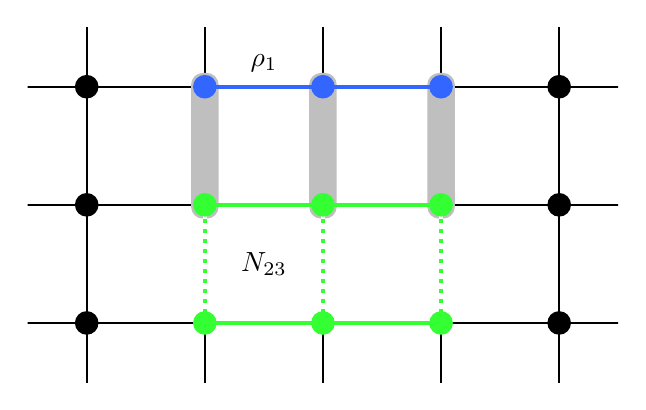
\begin{tikzpicture}[scale=0.5]
    % Define custom colors
\definecolor{customBlue}{rgb}{0.2, 0.4, 1}
\definecolor{customGreen}{rgb}{0.2, 1, 0.2}
\begin{scope}
\clip (-4.5,-1.5) rectangle (10.5,7.5);
\begin{scope}
    \foreach \x in {-6,-3,...,12} {
        \draw[thick, black] (\x,-3) -- (\x,9);
    }
    \foreach \y in {-3,0,...,9} {
        \draw[thick,black] (-6,\y) -- (12,\y);
    }
\end{scope}

    \fill[lightgray, rounded corners=0.15cm] (0-0.35,3+0-0.35) rectangle (0+0.35,6+0+0.35);
    \fill[lightgray, rounded corners=0.15cm] (3-0.35,3+0-0.35) rectangle (3+0.35,6+0+0.35);
    \fill[lightgray, rounded corners=0.15cm] (6-0.35,3+0-0.35) rectangle (6+0.35,6+0+0.35);

    \draw[customGreen, ultra thick] (0,0) -- (3,0) -- (6,0);  
    \draw[customGreen, ultra thick] (0,3) -- (3,3) -- (6,3);
    \draw[customBlue, ultra thick] (0,6) -- (3,6) -- (6,6);
    \draw[white, ultra thick] (0,0) -- (0,3);
    \draw[white, ultra thick] (3,0) -- (3,3);
    \draw[white, ultra thick] (6,0) -- (6,3);
    \draw[customGreen, ultra thick, dotted] (0,0) -- (0,3);
    \draw[customGreen, ultra thick, dotted] (3,0) -- (3,3);
    \draw[customGreen, ultra thick, dotted] (6,0) -- (6,3);


    \fill[black] (-3,0) circle (0.3);
    \fill[black] (-3,3) circle (0.3);
    \fill[black] (-3,6) circle (0.3);

    \fill[black] (9,0) circle (0.3);
    \fill[black] (9,3) circle (0.3);
    \fill[black] (9,6) circle (0.3);


    \fill[customGreen] (0,0) circle (0.3);
    \fill[customGreen] (3,0) circle (0.3);
    \fill[customGreen] (6,0) circle (0.3);

    \fill[customGreen] (0,3) circle (0.3);
    \fill[customGreen] (3,3) circle (0.3);
    \fill[customGreen] (6,3) circle (0.3);

    \fill[customBlue] (0,6) circle (0.3);
    \fill[customBlue] (3,6) circle (0.3);
    \fill[customBlue] (6,6) circle (0.3);

    \node[fill=white, inner sep=0pt] at (1.5,1.5) {$N_{23}$};
    \node at (1.5,6.6) {$\rho_1$};
\end{scope}
\end{tikzpicture}
}
\caption{ A tripartite graph state can be detected by preparing a network state, Bell measurements, and a fixed measurement. Entangled states of arrayed qubits can be detected by state preparation and a fixed measurement. }
\label{fig:chain}
\end{figure}

\begin{figure}
\centering
\resizebox{0.7\linewidth}{!}{
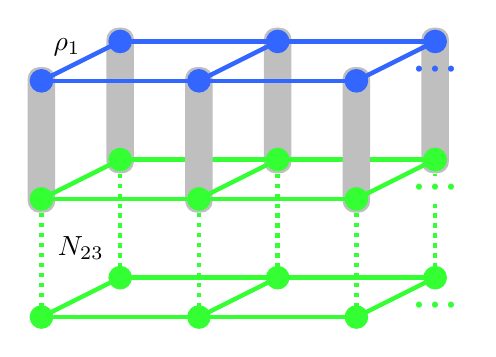
\begin{tikzpicture}[scale=0.5]
    % Define custom colors
    \definecolor{customBlue}{rgb}{0.2, 0.4, 1}
    \definecolor{customGreen}{rgb}{0.2, 1, 0.2}

    \fill[lightgray, rounded corners=0.15cm] (2-0.35,3+1-0.35) rectangle (2+0.35,6+1+0.35);
    \fill[lightgray, rounded corners=0.15cm] (6-0.35,3+1-0.35) rectangle (6+0.35,6+1+0.35);
    \fill[lightgray, rounded corners=0.15cm] (10-0.35,3+1-0.35) rectangle (10+0.35,6+1+0.35);

    \draw[customGreen, ultra thick] (0,0+0) -- (4,0+0) -- (8,0+0);  
    \draw[customGreen, ultra thick] (2,0+1) -- (6,0+1) -- (10,0+1); 
    \draw[customGreen, ultra thick] (0,0+0) -- (2,0+1);  
    \draw[customGreen, ultra thick] (4,0+0) -- (6,0+1);
    \draw[customGreen, ultra thick] (8,0+0) -- (10,0+1);

    \draw[customGreen, ultra thick] (2,3+1) -- (6,3+1) -- (10,3+1);

    \fill[lightgray, rounded corners=0.15cm] (0-0.35,3+0-0.35) rectangle (0+0.35,6+0+0.35);
    \fill[lightgray, rounded corners=0.15cm] (4-0.35,3+0-0.35) rectangle (4+0.35,6+0+0.35);
    \fill[lightgray, rounded corners=0.15cm] (8-0.35,3+0-0.35) rectangle (8+0.35,6+0+0.35);

    \draw[customGreen, ultra thick] (0,3+0) -- (4,3+0) -- (8,3+0);
    \draw[customGreen, ultra thick] (0,3+0) -- (2,3+1);
    \draw[customGreen, ultra thick] (4,3+0) -- (6,3+1);
    \draw[customGreen, ultra thick] (8,3+0) -- (10,3+1);
    
    \draw[customBlue, ultra thick] (0,6+0) -- (4,6+0) -- (8,6+0);
    \draw[customBlue, ultra thick] (2,6+1) -- (6,6+1) -- (10,6+1);
    \draw[customBlue, ultra thick] (0,6+0) -- (2,6+1);
    \draw[customBlue, ultra thick] (4,6+0) -- (6,6+1);
    \draw[customBlue, ultra thick] (8,6+0) -- (10,6+1);


    % First and second rows of disks
    \fill[customGreen] (0,0+0) circle (0.3);
    \fill[customGreen] (4,0+0) circle (0.3);
    \fill[customGreen] (8,0+0) circle (0.3);
    \fill[customGreen] (2,0+1) circle (0.3);
    \fill[customGreen] (6,0+1) circle (0.3);
    \fill[customGreen] (10,0+1) circle (0.3);

    \fill[customGreen] (0,3+0) circle (0.3);
    \fill[customGreen] (4,3+0) circle (0.3);
    \fill[customGreen] (8,3+0) circle (0.3);
    \fill[customGreen] (2,3+1) circle (0.3);
    \fill[customGreen] (6,3+1) circle (0.3);
    \fill[customGreen] (10,3+1) circle (0.3);

    \fill[customBlue] (0,6+0) circle (0.3);
    \fill[customBlue] (4,6+0) circle (0.3);
    \fill[customBlue] (8,6+0) circle (0.3);
    \fill[customBlue] (2,6+1) circle (0.3);
    \fill[customBlue] (6,6+1) circle (0.3);
    \fill[customBlue] (10,6+1) circle (0.3);

    \draw[customGreen, ultra thick, dotted] (0,0+0) -- (0,3+0);
    \draw[customGreen, ultra thick, dotted] (4,0+0) -- (4,3+0);
    \draw[customGreen, ultra thick, dotted] (8,0+0) -- (8,3+0);
    \draw[customGreen, ultra thick, dotted] (2,0+1) -- (2,3+1);
    \draw[customGreen, ultra thick, dotted] (6,0+1) -- (6,3+1);
    \draw[customGreen, ultra thick, dotted] (10,0+1) -- (10,3+1);

    \node at (10,0+0.25) [text=customGreen] {\huge \(\cdot\)\(\cdot\)\(\cdot\)};
    \node[fill=white, inner sep=0pt] at (10,3+0.25) [text=customGreen] {\huge \(\cdot\)\(\cdot\)\(\cdot\)};
    \node at (10,6+0.25) [text=customBlue] {\huge \(\cdot\)\(\cdot\)\(\cdot\)};

    \node[fill=white, inner sep=0pt] at (1,1.75) {$N_{23}$};
    \node at (0.65,6.85) {$\rho_1$};
\end{tikzpicture}
}
\caption{The estimation of entanglement witnesses for multipartite graph states.}
\label{graph state scheme}
\end{figure}

\subsection{ EWs for multipartite systems}

Thirdly, entanglement detection by state preparation can be extended to multipartite quantum states. We here, in particular, consider graph states, a class of states as a resource for MBQC \cite{PhysRevLett.86.5188}. Let us again present an instance for a three-qubit graph state, a Greenberger–Horne–Zeilinger (GHZ) state $|\psi\rangle = (|000\rangle +|111\rangle)/\sqrt{2}$ \cite{PhysRevA.62.062314}, see Fig. \ref{fig:chain}. An EW to detect a GHZ state may be given as,
\bea
W = \frac{1}{2} \mathbbm{1} - |\psi \rangle \langle \psi|.
\eea
A network state for an EW above can be constructed as,
\bea
N_{23} = \frac{1}{8} \sum_{a,b,c=0}^{1} \psi_{abc}^{(A_2 B_2 C_2)} \otimes \psi_{abc}^{(A_3 B_3 C_3)}.
\eea
where $\psi_{abc} = |\psi_{abc}\rangle \langle \psi_{abc}|$,
\bea
|\psi_{abc}\rangle = Z^a \otimes X^b \otimes X^c |\psi\rangle, ~~a,b,c \in \{0,1\}
\eea
with Pauli matrices $X$ and $Z$. It holds that
%\bea
%\tr[\rho W] =  8 \tr[\rho_1\otimes N_{23} P_{12} \otimes (\frac{\mathbbm{1}}{2} - |\psi \rangle\langle \psi |)_{3}], \nonumber
%\eea
\bea
{}_{A_3B_3C_3} \langle \psi |\rho_1 \otimes N_{23} ~P^{(12)} |\psi \rangle_{A_3B_3C_3} = \frac{1}{16} - \frac{1}{8}\tr[\rho W], \nonumber
\eea
which shows detection of a genuinely multipartite entangled state $\rho$ by finding that the left-hand-side is greater than $1/16$. Further generalization for detecting entangled $n$-qubit graph states is provided in Appendix. \\


\subsection{ To construct non-decomposable EWs }


Finally, let us investigate two entangled states defined by an EW. One denotes an entangled state $\rho_1$ detected by an EW, and the other $N_{23}$ realizing an EW by its preparation; see also Eq. (\ref{eq:ewm}). The result in Ref. \cite{PhysRevLett.96.150501} shows that an EW detects a set of entangled states that can activate its network state. Since a pair of PPT states cannot activate each other, either the states $\rho_1$ or $N_{23}$ must be non-PPT. Hence, a network state $N_{23}$ to detect a PPT entangled state $\rho_1$ should be non-PPT. We thus conclude that multipartite non-PPT entangled states can construct non-decomposable EWs, which are then highly non-trivial.
{
Note that non-PPT states can construct both decomposable and nondecomposable EWs, as shown in the example of reduction EWs, see Eq. \eqref{reductionEW}.
}
\\

{ \section{Robustness}
\label{sec:robust}

The framework for detecting entangled states in the subsection \ref{sec:gc} contains elements, the preparation of a network state and a fixed measurement for estimating a singlet fraction. We reiterate the relation between the estimation of an EW and the framework with a network state, 
\begin{align}
\tr[\rho W] = \alpha ~ \tr[\rho_1 \otimes N_{23} P^{(12)} (\eta \I - |\phi_{d}^+\rangle \langle \phi_{d}^+ | )_3 ],
\end{align}
for some $\alpha>0$. We here investigate the effect of noise on the preparation of a network state and a fixed measurement and show that the framework can unambiguously detect entangled states. That is, for separable states, the framework with noisy resources gives a non-negative expectation value. 


\begin{figure*}[t]
    \centering
    \includegraphics[scale=.18]{ fig4.pdf}
    \caption{  {Estimation of an EW in Eq. (\ref{eq:ewex}) can be realized in a circuit, where a network state in Eq. (\ref{eq:wr}) is realized and measurements in the computational basis are applied, see also Eq. (\ref{eq:ewr}). (1) A state for detecting entanglement, $|\psi^{-}\rangle$, is generated in registers $A_1B_1$. (2) A network state from an EW  is prepared to detect entanglement generated in $A_1B_1$. (3) A projection onto a state $|\phi^+\rangle $ is realized by collecting outcomes $00$ in registers $A_1A_2$. (4) A projection onto a state $|\phi^+\rangle $ is realized by collecting outcomes $00$ in registers $B_1B_2$. (5) Given outcomes $0000$ in registers $A_1B_1A_2B_2$, the singlet fraction is estimated in $A_3B_3$: a state in register $A_1B_1$ is entangled if the probability of outcomes $00$ in $A_3B_3$ is larger than $1/2$.  }}
    \label{fig:4}
\end{figure*}


\subsubsection*{ Noisy network states }
Suppose that the network states $N$ is noisy such that
\begin{align*}
\widetilde N &= (1-p) N + p \frac{\I}{d^{2n}},
\end{align*}
with some noise fraction $p$. It follows that,
\bea
&&\alpha~ \tr[\rho_1 \otimes \widetilde N_{23} P^{(12)} (\eta \I -  |\phi_{d}^+\rangle \langle \phi_{d}^+ | )_3 ] \nonumber \\
%&=&  \tr[\rho_1 \otimes ((1-p) N + p \frac{\I}{d^{2n}})_{23} P^{(12)} (\eta \I - \psi)_3 ]  \nonumber \\
&=& (1-p) \tr[\rho W] + \alpha p \frac{1}{d^{2n}} \frac{1}{d^{n}} (\eta d^n-1) \nonumber \\
&\geq & (1-p) \tr[\rho W]. \nonumber
\eea
Note that the term apart from $\tr[\rho W]$ in the second line is not negative since $\eta\leq 1/d$. Hence, noisy network states can be used to detect entangled states unambiguously. 



\subsubsection*{White noise in singlet fraction estimation}
Suppose that a fixed measurement setting for estimating a singlet fraction is noisy,
\begin{align}
(1-q)  |\phi_{d}^+\rangle \langle \phi_{d}^+ | + q \frac{\I}{d^n} \nonumber
\end{align}
with some noise fraction $q$. It follows that
\bea
&& \alpha ~ \tr[\rho_1 \otimes N_{23} P^{(12)} (\eta \I - (1-q)  |\phi_{d}^+\rangle \langle \phi_{d}^+ | - q \frac{\I}{d^n}  )_3 ]  \nonumber \\
 &= & (1-q)\tr[\rho W] + \alpha q \frac{1}{d^n} (\eta - \frac{1}{d^n} \tr[\rho^T N] ) \nonumber \\
 &\geq & (1-q) \tr[\rho W]. \nonumber
\eea
Thus, when a fixed measurement setting is noisy, the framework gives non-negative expectation values for separable states.

% \subsection{White noise in local Bell measurements}
% Now suppose that the local Bell measurements $P_{00}$ are replaced by  
% \begin{align*}
% \widetilde P = (1-r) P_{00} + r \frac{\I}{2^2}, % \label{noisy P}
% \end{align*}
% with the noise fraction $r$.
% With the noisy local Bell measurements, the state of interest $\rho$ is detected by MBEW if
% \begin{align}
% 0 &> \tr[\rho_1 \otimes N_{23} (\widetilde{P}\power{n})_{12} \otimes (\frac{1}{2}\I - \dyad{\vo}_G)^{(S'')}] \lb
% &= \tr \bigg[\rho_1 \otimes N_{23} (\frac{1}{2}\I - \dyad{\vo}_G)^{(S'')} \otimes \lb
% &\phantom{= \tr \bigg[} \left( \sum_{k=0}^{n} \binom{n}{k} q^{n-k} (\frac{1-q}{2^2})^k P_{00}\power{n-k} \otimes \I\power{k} \right)^{(SS')} \bigg] \lb
% &= \frac{1}{2^n} \tr \bigg[\rho_1 \otimes (\frac{1}{2}\I - \dyad{\vo}_G)^{(S')} \lb
% & \phantom{= \frac{1}{2^n} \tr\bigg[} \left( \sum_{k=0}^{n} \binom{n}{k} q^{n-k} (\frac{1-q}{2^2})^k P_{00}\power{n-k} \otimes \I\power{k} \right)^{(SS')} \bigg] \label{Bell noise exact}
% \end{align}
% It is too complicated to calculate exact value of the expression in the Ineq. (\ref{Bell noise exact}). Instead, let us consider an upper bound of the expression given by the worst case: the measurements are $P_{00}\power{n}$  (success) with a probability $q^n$, and $(\frac{\I}{2^2})\power n$ (fail) with a probability $1-q^n$. Then, the state $\rho$ is detected when
% \begin{align}
% \frac{1}{2^n} \left( q^n \frac{1}{2^n} \tr[\rho W] + (1-q^n) \frac{1}{2^{2n}} (\frac{1}{2} 2^n -1) \right) < 0,
% \end{align}
% which implies 
% \begin{align}
% \tr[\rho W] < (\frac{1}{2} - \frac{1}{2^n}) (1 - \frac{1}{q^n}).
% \end{align}
% }


\section{Realization in quantum circuits}


The framework of detecting entangled states by a fixed measurement can be realized in a quantum circuit. Here, we demonstrate the realization of a network state and the estimation of an EW with an example in Eq. (\ref{eq:ewex}). To facilitate the construction of a quantum circuit, we exploit a decomposition of the network state in the following, 
\begin{align}
N_{23} &= \frac{1}{4} \big( \ketbra{\psi^-}_{A_2 B_2} \otimes \ketbra{\phi^+}_{A_3 B_3}  \nonumber \\
&~~~~~~ + \ketbra{\psi^+}_{A_2 B_2} \otimes \ketbra{\psi^+}_{A_3 B_3} \nonumber \\
&~~~~~~ + \ketbra{\phi^-}_{A_2 B_2} \otimes \ketbra{\phi^-}_{A_3 B_3} \nonumber \\
&~~~~~~ + \ketbra{\phi^+}_{A_2 B_2} \otimes \ketbra{\psi-}_{A_3 B_3} \big), 
\end{align}
which is identical to the state in Eq. \eqref{eq:wr}. Then, a circuit for realizing the network state is shown in Fig. \ref{fig:4}, where blocks (1)-(5) describe realizations of a network state, projection on a state $|\phi^+\rangle$, measurements of estimating the singlet fraction. We remark that a fixed measurement setting is used for estimating an EW. 

Considering the effect of noise in Section \ref{sec:robust}, one may expect that the framework can be realized in a noisy implementation of quantum information processing. We then implemented the circuit in the IBMQ Kyiv on April 2, 2025. The results are presented in Fig. \ref{fig:result}, demonstrating the robustness of the proposed framework for estimating EWs in a realistic setting. Although noise is present, the estimation of an EW shows a singlet fraction $0.61$ higher than the threshold $1/2$, detecting the presence of an entangled state in registers $A_1B_1$.


%\begin{figure}[t]
%\centering
%\[
%\Qcircuit @C=1em @R=.7em @!R {
%\lstick{A_1} & \gate{H} & \ctrl{1} & \gate{Z} & \qw        & \qw        & \ctrl{2} & \gate{H} & \qw      & \qw      & \meter & \cw \\
%\lstick{B_1} & \qw      & \targ    & \gate{X} & \qw        & \qw        & \qw      & \qw      & \ctrl{2} & \gate{H} & \meter & \cw \\
%\lstick{A_2} & \gate{H} & \ctrl{1} & \gate{Z} & \qw        & \qw        & \targ    & \qw      & \qw      & \qw      & \meter & \cw \\
%\lstick{B_2} & \qw      & \targ    & \gate{X} & \targ      & \ctrl{0}   & \qw      & \qw      & \targ    & \qw      & \meter & \cw \\
%\lstick{A_3} & \gate{H} & \qw      & \qw      & \ctrl{-1}  & \qw        & \gate{H} & \ctrl{1} & \ctrl{1} & \gate{H} & \meter & \cw \\
%\lstick{B_3} & \gate{H} & \qw      & \qw      & \qw        & \ctrl{-2}  & \qw      & \targ    & \targ    & \qw      & \meter & \cw \\
%}
%\]
%    \caption{ The quantum circuit for detection of $\ket{\psi^-}_{A_1 B_1}$ using a pure network state $\ket{N}_{A_2B_2A_3B_3}$, which implements the EW $W = \tfrac{1}{2} \I - \psi^-$ \eqref{eq:ewex}. The first three layers in $A_1 B_1$ generate $\ket{\psi^-}$ state, while first five layers within $A_2 B_2 A_3 B_3$ generate $N$. The CNOT gates followed by $H$ gate and measurements in $A_1 A_2$ and $B_1 B_2$ implements local Bell projections. The measuremnet outcome $0000$ for the first four bits corresponds to the $\phi^+$ projections on both sides.}
 %   \label{fig:flip EW circuit}
%\end{figure}

\begin{figure}[t]
    \centering
    \includegraphics[scale=.13]{ fig5.pdf}
    \caption{ { The circuit in \ref{fig:4} is run in the IBMQ Kyiv. Given outcomes $0000$ in registers $A_1A_2B_1B_2$, the singlet fraction in registers $A_3B_3$ corresponds to the probability of having an outcome $00$. While $10000$ counts are obtained for registers $A_1A_2A_3B_1B_2B_3$, we have $685$ counts for $0000$ on $A_1A_2B_1B_2$, given which we have the singlet fraction $0.61$ which is larger than $1/2$. While the IBMQ Kyiv is noisy, we have demonstrated the generation and the detection of entangled states on a quantum circuit. 
    }}
    \label{fig:result}
\end{figure}

\section{Conclusion}


In conclusion, we have established an MB framework for estimating observables, in particular EWs, and shown the construction of network states for observables. It is also of fundamental interest to find that entanglement demonstrates elements of quantum theory, both dynamics, i.e., MBQC and observables. Our results shed new light on detecting and manipulating entangled states in a realistic scenario where precise controls via quantum gates are yet limited, such as an array of superconducting qubits, neutral atoms, or photons, where the preparation of a multipartite state and a fixed measurement are readily experimentally feasible. The results also open a new avenue of exploiting entangled states in distributed quantum information processing such as computing and metrology where entanglement is resourceful and quantum estimation {\it per se} corresponds to computing or metrology. 

In future directions, it would be interesting to realize the estimation of EWs via network states experimentally by considering the effects of noise in a realistic setting. Note that some network states, such as Smolin, have been realized in experiment \cite{Amselem:2009aa, PhysRevLett.105.130501, PhysRevLett.109.040501}. It is also interesting to exploit network states in a network and security scenario such as a measurement-device-independent scenario, see Refs. \cite{PhysRevLett.108.200401,PhysRevLett.110.060405}, so that observables such as EWs are estimated by relaxing assumptions on joint measurements; estimation of EWs, as well as detection of entanglement, is achieved in a higher level of robustness against imperfect implementations. 

\section*{Acknowledgement}

This work is supported by National Research Foundation of Korea (NRF-2021R1A2C2006309, NRF-2022M1A3C2069728) and the Institute for Information \& Communication Technology Promotion (IITP) (RS-2023-00229524, the ITRC Program/IITP-2023-2018-0-01402). AB and DC were supported by the Polish National Science Center project No. 2018/30/A/ST2/00837.


\bibliographystyle{quantum}
% \bibliography{bibedsp}
% \documentclass[a4paper,twocolumn,11pt,accepted=2017-05-09]{quantumarticle}
\documentclass[a4paper,twocolumn,10pt]{quantumarticle}
\pdfoutput=1
\usepackage[utf8]{inputenc}
\usepackage[english]{babel}
\usepackage[T1]{fontenc}
\usepackage{amsmath}
\usepackage{hyperref}

\usepackage{tikz}
\usepackage{lipsum}

\newtheorem{theorem}{Theorem}


\usepackage{tikz}
\usepackage{qcircuit}
%%%%%%%%%%%%%%%%%%

%\usepackage{IEEEtrantools}
\usepackage{multirow}

% ------------------------------------------------------------------------------
\newcommand{\rev}{\color{blue}}
\newcommand{\bae}{\color{purple}}
\newcommand{\ji}{\color{gray}}

\newcommand{\vx}{\Vec{x}}
\newcommand{\vy}{\Vec{y}}
\newcommand{\vo}{\Vec{0}}
\newcommand{\Va}{\Vec{a}}
\newcommand{\Vb}{\Vec{b}}
\newcommand{\power}[1]{^{\otimes #1}}
\newcommand{\lb}{\nonumber \\}


\newcommand{\R}{\mathbb{R}}
\newcommand{\N}{\mathbb{N}}
\newcommand{\C}{\mathbb{C}}
\newcommand{\Z}{\mathbb{Z}}
\newcommand{\Q}{\mathbb{Q}}
\newcommand{\I}{\mathbbm{1}}

\newcommand{\tr}{\text{tr}}
\newcommand{\ket}[1]{| #1 \rangle}
\newcommand{\bra}[1]{\langle #1|}
\newcommand{\ip}[2]{\langle #1|#2 \rangle}
\newcommand{\bracket}[3]{\langle #1|#2|#3 \rangle}
\newcommand{\sm}[1]{\left( \begin{smallmatrix} #1 \end{smallmatrix} \right)}

\newcommand{\be}{\begin{equation}}
\newcommand{\ee}{\end{equation}}
\newcommand{\bea}{\begin{eqnarray}}
\newcommand{\eea}{\end{eqnarray}}
\newcommand{\bes}{\begin{equation*}}
\newcommand{\ees}{\end{equation*}}
\newcommand{\beas}{\begin{eqnarray*}}
\newcommand{\eeas}{\end{eqnarray*}}

% ------------------------------------------------------------------------------

\newcommand{\x}{\mathrm{x}}
%\newcommand{\ket}[1]{|#1\rangle}
\newcommand{\ketbra}[1]{\ket{#1}\!\bra{#1}}
%\newcommand{\bra}[1]{\langle#1|}
\newcommand{\dyad}[1]{\ket{#1}\!\bra{#1}}

\newcommand{\ten}{\otimes}
\newcommand{\Id}{\mathds{1}}
\newcommand{\zero}{\mathbf{0}}
\newcommand{\KBDS}{C^{s}}
\newcommand{\KBDSs}{C}
%\newcommand{\KBDS}{C^{\mbox{\tiny U}}}
\newcommand{\KTwo}{C^{2\times2}}
\renewcommand{\H}{\mathcal{H}}
\def\A{\mathcal{A}}
\def\B{\mathcal{B}}

\def\x{\mathrm{x}}
\def\y{\mathrm{y}}

\def\W{\mathcal{W}}


\def\sig{\widetilde{\sigma}}
\def\F{\mathcal{F}}
\def\N{\mathcal{N}}
\def\P{\mathbbm{P}}
\def\tr{\mathrm{tr}}

\def\L{\mathcal{L}}
\def\Q{\mathcal{Q}}
\def\NL{\mathcal{NS}}

\DeclareMathOperator*{\Oplus}{\bigoplus}
\DeclareMathOperator*{\Otimes}{\bigotimes}
% \DeclareMathOperator*{\Oplus}{\scalerel*{\bigoplus}{\textstyle\sum}}
% ------------------------------------------------------------------------------






\begin{document}

\title{ Detecting Entanglement by State Preparation and Local Measurements}


\author{Jaemin Kim}
\email{woals6584@kaist.ac.kr}
\affiliation{School of Electrical Engineering, Korea Advanced Institute of Science and Technology (KAIST), 291 Daehak-ro, Yuseong-gu, Daejeon 34141, Republic of Korea }
\orcid{ }


\author{Anindita Bera}
\email{aninditatitli@gmail.com}
\affiliation{Department of Mathematics, Birla Institute of Technology Mesra, Jharkhand 835215, India}
\orcid{ }


\author{Dariusz Chru\'sci\'nski}
\email{darch@fizyka.umk.pl}
\affiliation{Institute of Physics, Faculty of Physics, Astronomy, and Informatics, Nicolaus Copernicus University, Grudziadzka 5, 87-100 Torun, Poland}
\orcid{ }

\author{Joonwoo Bae}
\email{joonwoo.bae@kaist.ac.kr}
\affiliation{School of Electrical Engineering, Korea Advanced Institute of Science and Technology (KAIST), 291 Daehak-ro, Yuseong-gu, Daejeon 34141, Republic of Korea }
\orcid{ }


\maketitle

\begin{abstract}
  Entanglement witnesses (EWs) are a collection of observables that can characterize separable states and, experimentally, estimating EWs can verify entangled states. In this work, we show that a fixed measurement setting on a multipartite entangled state, which we introduce as a \emph{network state} for the purpose, can estimate EWs. Namely, entangled states can be fully verified in a measurement-based manner, in which experimenters do not necessarily change measurement settings. We present a fixed measurement setting and network states for estimating decomposable EWs, equivalent to the partial transpose criteria. We also consider non-decomposable EWs that detect bound entangled states beyond the partial transpose criteria. The results can be extended to multipartite states such as graph states, a resource for measurement-based quantum computing, and readily applied to distributed settings such as quantum metrology or sensor networks where multipartite entangled states are resourceful.
\end{abstract}





\section{Introduction}


{Entangled states are a key resource in quantum information processing, in particular, to achieve quantum advantages in computation and communication tasks. A higher level of security in cryptographic protocols \cite{PhysRevLett.98.230501}, higher level of quantum certification \cite{Pironio_2009, PhysRevLett.110.060405, PhysRevLett.108.200401, Bowles:2018aa} and higher network channel capacities \cite{PhysRevA.95.052329, PhysRevLett.125.150502} can be achieved by exploiting entangled states. Efficient computation with quantum resources can be realized by local measurements and entangled states only, called measurement-based quantum computation (MBQC) \cite{PhysRevLett.86.5188, MeasurementBasedQuantumComputation, Briegel:2009aa}. }

{ Entanglement witnesses (EWs) \cite{TERHAL2000319, PhysRevA.62.052310} are versatile tools to detect entangled states both theoretically and experimentally. They correspond to observables that are non-negative for all separable states but negative for some entangled states \cite{HORODECKI19961, GUHNE20091, RevModPhys.81.865, Chru_ci_ski_2014, Friis:2019aa}. Hence, negative expectation values of EWs unambiguously conclude the presence of entangled states. In practice, multiple measurement settings may be necessary for estimating EWs. }

{ In this work, we show that a fixed measurement setting can detect entangled states, together with the preparation of a multipartite state, which we call a {\it network state}. To be precise, we present a framework for detecting entangled states such that a fixed measurement over a network state $N$ and a state $\rho$ can find if the state $\rho$ is entangled, where a network state $N$ is obtained from an EW. Thus, entangled states can be verified in a measurement-based (MB) manner. In fact, the framework is closely connected to the activation of entanglement in that it finds if a state $\rho$ is entangled if a joint state $N\otimes \rho$ is more entangled than a state $N$. }

We show how network states can be obtained from EWs. We present the construction of network states for decomposable EWs, which are equivalent to the partial transpose criteria, and also for non-decomposable EWs that detect bound entangled states beyond the partial transpose criteria, such as the Bell-diagonal EWs \cite{chruscinski2014class, PhysRevA.105.052401} from the Choi map \cite{Choi:1975aa} and its various generalizations \cite{PhysRevA.84.024302}, and the Breuer-Hall EW \cite{PhysRevLett.97.080501, Hall_2006}. The results are extended to multipartite systems: graph states \cite{PhysRevA.69.062311}, a resource for MBQC \cite{PhysRevLett.86.5188}, can be detected by network states and a fixed measurement.
{ 
We discuss the connection of our work to the entanglement activation \cite{PhysRevLett.96.150501} and the measurement-device-independent entanglement witnesses \cite{PhysRevLett.110.060405}.
}

The importance of our results is threefold. Firstly, similarly to MBQC, one can circumvent the control of multiple measurement settings when estimating observables. Precise controls on and the preparation of general measurements identify additional difficulties for realizing EWs in general. Our results show that the preparation of quantum states and a fixed measurement can be an experimentally feasible alternative. Secondly, it is of fundamental interest to find that entangled states with a fixed measurement are a resource that can be replaced with observables. Note that MBQC signifies that entangled states and local measurements can be an alternative to realize quantum state transformation. Finally, the framework for estimating EWs in an MB manner finds various usefulness of distributed settings such as distributed quantum metrology over networks, e.g., \cite{Chabuda:2020aa, Zhang_2021,Len:2022aa, PhysRevLett.121.043604}: estimation of joint observables enables distributed quantum information processing, e.g., \cite{PhysRevA.85.062326, Friis_2017, PhysRevLett.120.080501}.

\section{Entanglement detection}
 
Let us begin by describing an experimental scenario of verifying entangled states, where the scenario is common in various experimental settings. We consider two quantum systems $A$ and $B$ on a Hilbert space $\H\otimes \H$. Interestingly, observables exist, denoted by $W=W^{\dagger}$, such that, for all separable states $\sigma_{\mathrm{sep}}$, 
\bea
\tr[W\sigma_{\mathrm{sep}}] \geq 0~~\mathrm{and }~~ \tr[W\rho_{\mathrm{ent}}] <0\nonumber
\eea
for some entangled states $\rho_{\mathrm{ent}}$ \cite{TERHAL2000319, PhysRevA.62.052310}. All entangled states can be verified by estimating some observables, which are called entanglement witnesses (EWs). In experiment, EWs can be estimated by altering measurement settings in general: negative expectation values unambiguously conclude entangled states \cite{GUHNE20091}. They can be also used to verify other properties, other than entanglement, such as a fidelity in the state preparation \cite{PhysRevA.76.030305, Haffner:2005aa}.

%Note that the structure of EWs remains } 


%One of the intriguing properties of entangled states is the irreversibility in manipulations of entanglement. Entangled states from which no entanglement can be extracted, though entanglement is needed for their preparation, are identified as {\it undistillable} or {\it bound} entangled states \cite{PhysRevA.61.062313, PhysRevLett.86.2681}. Multipartite quantum states that remain positive after partial transpose (PPT) turn out to be undistillable. Remarkably, PPT entangled states can be used to activate other entangled states \cite{horodecki1999bound}.

%Then, non-PPT entangled states can be characterized by decomposable EWs that have a general form as follows,
%\bea
%W = P+Q^{\Gamma},~~\mathrm{for}~~P,~Q\geq 0\nonumber.
%\eea
%Here $\Gamma$ denotes the partial transpose. Then, non-decomposable EWs, which cannot be in the form above, can detect PPT entangled states. 

%\cite{PhysRevA.61.062313, PhysRevLett.86.2681}.

%In general, it is highly non-trivial to construct non-decomposable EWs, which are the main object in the mathematically challenging problem of classifying positive linear maps of Operator Algebras \cite{Stormer:1963aa}, see also Refs. \cite{bera2022generalizing, bera2022class,mirror}.

{\section{Measurement-Based Estimation}

Let us show that observables can be generally estimated in a measurement-based manner. We here focus on EWs, observables of particular interest for detecting entangled states, and provide the scheme for estimating of single observables in Appendix. We devise multipartite quantum states, {\it called network states}, for estimating observables. 

\subsection{Example }
\label{subsec:ex}
Let us begin with an illuminating example of an MB estimation of an EW. Throughout, Bell states are denoted by $|\phi^{\pm}\rangle = (|00\rangle \pm |11\rangle)/\sqrt{2}$ and $|\psi^{\pm}\rangle = (|01\rangle \pm |10\rangle)/\sqrt{2}$. We consider an EW in the following,
\bea
%W = \frac{1}{2} \mathbbm{1} - |\psi^{-} \rangle \langle \psi^{-} |, \nonumber
W = \frac{1}{4} (\mathbbm{1} + X\otimes X + Y\otimes Y + Z\otimes Z) \label{eq:ewex}
\eea
where $X,Y$ and $Z$ are Pauli matrices. Eq. (\ref{eq:ewex}) shows that an EW can be estimated by various measurement settings. Note that a Bell state $|\psi^{-}\rangle$ is detected by an EW above. 
 
 
%\subsection{Two-qubit network states}

The MB framework for estimating an observable in Eq. (\ref{eq:ewex}) can be achieved by a four-partite state, called a {\it network state}, constructed as follows, 
\bea
N_{23} &=& \frac{1}{4} |\psi^-\rangle_{A_2B_2} \langle \psi^-| \otimes |\phi^+\rangle_{A_3B_3} \langle \phi^+| + \nonumber \\
&&\frac{1}{12} (\mathbbm{1} - |\psi^-\rangle_{A_2B_2} \langle \psi^-|) \otimes (\mathbbm{1} - |\phi^+\rangle_{A_3B_3} \langle \phi^+|),~~~~ ~\label{eq:wr}
\eea

on sites $A_2A_3B_2B_3$, see Fig. \ref{fig:fig1}. We then place a state of interest at $A_1B_1$, denoted by $\rho_{1}:=\rho^{( A_1B_1)}$, which we want to learn if it is entangled. We have
\bea
\tr[\rho W ] =  16~ \tr  [\rho_1\otimes N_{23} (\frac{1}{2}\mathbbm{1} - | \phi^+\rangle_{A_3B_3} \langle \phi^+|) \otimes P^{(12)}],~~
\label{eq:ewr}
\eea
where $P^{(12 )} = |\phi^{+}\rangle_{A_1A_2}\langle \phi^+| \otimes |\phi^{+}\rangle_{B_1B_2}\langle \phi^+|$. Eq. (\ref{eq:ewr}) can be simplified by a singlet fraction as follows,
\bea
_{A_3 B_3}  \langle \phi^{+}| \tr_{12}[ \rho_1 \otimes N_{23} ~P^{(12)} ]  |\phi^{+}\rangle_{A_3 B_3}   = \frac{1}{8} - \frac{1}{4}\tr[\rho W].~~
\label{eq:expew}
\eea
The left-hand-side can be obtained by preparing a network state followed by a fixed measurement. A state $\rho_1$ is entangled if the right-hand-side is greater than $1/8$ since $\tr[\sigma_{\mathrm{sep}}W ]\geq 0 $ for all separable states $\sigma_{\mathrm{sep}}$. Once a Bell measurement reports an outcome $P^{(12)} $, a singlet fraction is estimated from the probability of having outcome $|\phi^{+}\rangle$ on $A_3B_3$. Thus, it is shown that an EW can be estimated in a fully MB manner. 

%In fact, an entangled state $\rho$ is detected if the probability, i.e., the left-hand-side in Eq. (\ref{eq:expew}), is greater than $1/8$, since $\tr[\sigma_{\mathrm{sep}}W ]\geq 0 $ for all separable states $\sigma_{\mathrm{sep}}$.


Experimental resources to realize the MB framework, i.e., the left-hand side in Eq. (\ref{eq:expew}), are as follows. A network state is required, see Eq. (\ref{eq:ewex}), which is entangled and bi-separable. The detection scheme needs a measurement in the basis $|\phi^+\rangle$, which is equivalent to the capability of realizing a controlled-NOT gate, a Hadamard gate, and a fixed-measurement in the $z$-direction; see also Fig. \ref{fig:fig1}. All these are compatible with the resources to realize MBQC. In addition, it is worth mentioning that a network state in Eq. (\ref{eq:wr}) is a variation of a Smolin state, a four-partite bound entangled state \cite{PhysRevA.63.032306}, which has been repeatedly realized in experiment \cite{ Amselem:2009aa, PhysRevLett.105.130501, PhysRevLett.109.040501}. It should be pointed out that a realization of the presented MB framework is readily available in an experiment. 



\begin{figure}[t]
\centering
% \includegraphics[width=9.0cm ]{figure1}
\resizebox{0.9\linewidth}{!}{
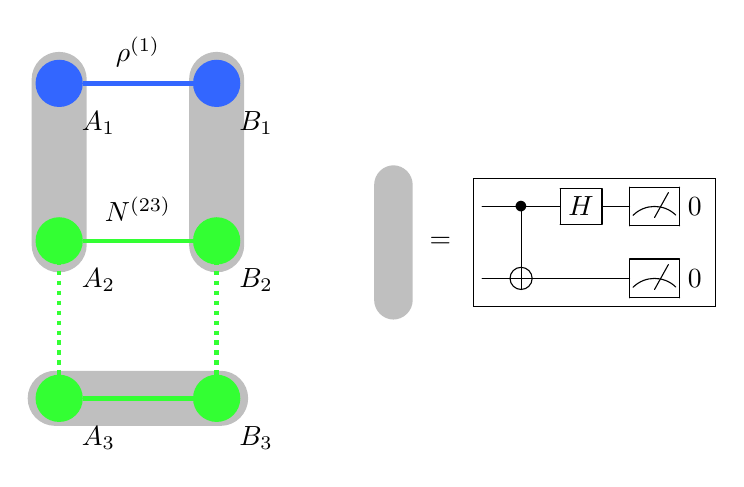
\begin{tikzpicture}[scale=2]
    % Define custom colors
    \definecolor{customBlue}{rgb}{0.2, 0.4, 1}
    \definecolor{customGreen}{rgb}{0.2, 1, 0.2}

    % Round-edged rectangles and dotted lines for both rows
\fill[lightgray, rounded corners=0.35cm] (-0.175,1.2) rectangle (0.175,-0.2);
\fill[lightgray, rounded corners=0.35cm] (-1-0.175,1.2) rectangle (-1+0.175,-0.2);
\fill[lightgray, rounded corners=0.35cm] (-0.5-0.7,-0.825) rectangle (-0.5+0.7,-1.175);
\draw[customGreen, ultra thick, dotted] (0,0) -- (0,-1);
\draw[customGreen, ultra thick, dotted] (-1,0) -- (-1,-1);

% Green ultra thick lines between A2-B2 and A3-B3
\draw[customGreen, ultra thick] (0.15,0) -- (-1+0.15,0);
\draw[customGreen, ultra thick] (0.15,-1) -- (-1+0.15,-1);

% Blue ultra thick line between A1 and B1
\draw[customBlue, ultra thick] (0.15,1) -- (-1+0.15,1);

    % First row of disks
    \fill[customBlue] (0,1) circle (0.15);
    \fill[customGreen] (0,0) circle (0.15);
    \fill[customGreen] (0,-1) circle (0.15);

    % Second row of disks
    \fill[customBlue] (-1,1) circle (0.15);
    \fill[customGreen] (-1,0) circle (0.15);
    \fill[customGreen] (-1,-1) circle (0.15);

    % Captions
    \node at (-0.5,1.2) {$\rho^{(1)}$};
    \node at (-0.5,0.2) {$N^{(23)}$};

% Labels
\node at (-1+0.25,0.75) {$A_1$};
\node at (-1+0.25,-0.25) {$A_2$};
\node at (-1+0.25,-1.25) {$A_3$};
\node at (+0.25,0.75) {$B_1$};
\node at (+0.25,-0.25) {$B_2$};
\node at (+0.25,-1.25) {$B_3$};

    \begin{scope}[xshift=1cm, yshift=-0.5cm, scale=0.7] % Adjust yshift for spacing between figures
        \fill[lightgray, rounded corners=0.25cm] (0,0) rectangle (0.35,1.4);

        \node at (0.6,0.7) {$=$};

        % Quantum Circuit inside a TikZ node
        \node[draw, inner sep=3pt] at (2,0.7) {
            \Qcircuit @C=1em @R=1.2em {
            % Qubit setup
            \lstick{} & \ctrl{1} & \gate{H} & \meter & \rstick{\hspace{-1.2em} 0} \\
            \lstick{} & \targ    & \qw      & \meter & \rstick{\hspace{-1.2em} 0} \\
            }
        };
    \end{scope}
\end{tikzpicture}
}
\caption{ A four-partite network state $N_{23}$ is prepared on $A_2A_3B_2B_3$ to detect an entangled state on $A_1B_1$. Bi-interactions and measurements in the computational basis can construct EWs, see also Eq. (\ref{eq:expew}) in the text. Gray boxes denote a measurement in the basis $|\phi^{+}\rangle$, which is equivalent to a measurement in the computational basis after applying of a controlled-NOT gate followed by a Hadamard gate. }
\label{fig:fig1}
\end{figure}



\subsection{ EWs via entanglement activation}

To show a general construction of network states for arbitrary EWs for high-dimensional quantum systems, we want to clarify their relations to activation of entanglement \cite{PhysRevLett.96.150501}: all EWs can be expressed in the following form, }
\bea
W_{A_2 B_2 } = \tr_{A_3B_3} \big[N (\eta \mathbbm{I} - |\phi_{d}^+ \rangle_{A_3B_3} \langle \phi_{d}^+ |)\big], \label{eq:ewm}
\eea
for some network state $N := N^{(A_2 B_2 A_3 B_3)}$ and a parameter $\eta \in [1/d,1 )$, where $|\phi_{d}^+\rangle = \sum_{j=0}^{d-1}|jj\rangle /\sqrt{d}$. It is worth mentioning an EW above shares similarity with Eq. (\ref{eq:ewr}) Note that the parameter $\eta$ satisfies the condition, $\eta\geq E_d [N]$ where $E_d$ is called a maximal singlet fraction,
\bea
E_d[N] &=& \sup_{\F}~ \langle \phi_{d}^+| \F[ N ] |\phi_{d}^+\rangle ~\mathrm{for~a~local ~filtering~}\F   \nonumber \\
&& \F[N] = \frac{ K_{A}\otimes K_B N K_{A}^{\dagger}\otimes K_{B}^{\dagger} }{ \tr[  K_{A}^{\dagger}K_{A} \otimes K_{B}^{\dagger}K_{B} N ]},\label{eq:fil}
\eea
where $K_A: \H_{A_1A_2}\rightarrow \mathbbm{C}^d $ and $K_B: \H_{B_1B_2}\rightarrow \mathbbm{C}^d $. It is worth mentioning that EWs in Eq. (\ref{eq:ewm}) identify entangled states that activate a network state in the sense that
\bea
E_d[ \sigma\otimes N]>\eta, ~\mathrm{whereas}~ {E_d [N]\leq \eta}.\label{eq:ac}
\eea
In fact, all entangled states can be used to activate some other state: in Eq. (\ref{eq:ac}) a state $\sigma$ is entangled if and only if it can activate some other entangled state $N$.



{ 
\subsection{ Detection protocol from  entanglement activation}

We exploit the scenario of activating entanglement as a framework for detecting entangled states. Namely, a state $\rho$ is entangled if it can be used to activate a state $N$. To this end, we consider a local filtering operation $\Phi$ as follows,
\begin{align}
\Phi (\rho \otimes N) = \tr_{A_1 B_1 A_2 B_2}[ P^{(12)} \rho^{(A_1 B_1)} \otimes N^{(A_2 B_2 A_3 B_3)}]. \nonumber
\end{align}
where $P^{(12)}$ the projection onto maximally entangled states as follows,
\bea
P^{(12 )} = |\phi_{d}^{+}\rangle_{A_1A_2}\langle \phi_{d}^+| \otimes |\phi_{d}^{+}\rangle_{B_1B_2}\langle \phi_{d}^+| \label{eq:projd} 
\eea
and $|\phi_{d}^+\rangle = \sum_{i=1}^d|ii\rangle/\sqrt{d}$. The singlet fraction after the filtering operation is given by,
\begin{align}
F_{\Phi}(\rho \otimes N) = \frac{ \bracket{\phi_d^+}{\Phi(\rho \otimes N)}{\phi_d^+} }{\tr[\Phi(\rho \otimes N)]}.\nonumber
\end{align}
With the specific local operation, the singlet fraction of a network state $N$ can be computed as, 
\begin{align}
\widetilde E_d(N) = \sup_{\sigma \in \mathrm{SEP}} F_{\Phi}(\sigma \otimes N),
\end{align}
where $\mathrm{SEP}$ denotes the set of separable states. It is clear that $\widetilde E_d(N) \le E_d(N)$ since a specific local operation is considered. Note also that for $\eta \in [\frac{1}{d},1)$, there exists a state $N$ such that $E_d(N) = \widetilde E_d(N) = \eta$ \cite{PhysRevLett.96.150501}. It holds that a state $\rho$ is entangled if we have $F_{\Phi}(\rho \otimes N) > \eta $ for $N$ such that $\widetilde E_d(N) \leq \eta$. 
}




\subsection{ General construction of network states }
\label{sec:gc}

Let us then present a construction of a network state for a given EW, see also Eq. (\ref{eq:ewm}). Suppose that an EW on $d\otimes d$ is decomposed as follows,
\bea
W = \sum_{j} a_j W(j)^T ~\mathrm{with}~ W(j) \geq 0 ~\mathrm{and}~ a_j \in \mathbbm{R}, \label{eq:eeww}
\eea
so that one can choose normalized non-negative operators $\{ \Pi(i) \geq 0\}$ and real constants $\{ c_j\}$ such that,
\bea
N_{23} &=&\sum_{j} c_j  W(j)_{A_2B_2} \otimes  \Pi(j)_{A_3B_3}, ~\mathrm{and}  \label{eq:ns} \\
W_2 & =& ~ k \, \tr_{3} [N_{23}^{T_2}  ( \eta \mathbbm{1} - |\phi_{d}^+ \rangle_{A_3B_3} \langle \phi_{d}^+ |  )  ], \label{eq:ewn}
\eea
for some $\eta\geq 1/d$ and $k>0$, where $W_2$ reproduces a given EW in Eq. (\ref{eq:eeww}) on sites $A_2 B_2$. One can find $\{a_j\}$ and $\{c_j \}$ are related as follow,
\bea
a_j = k \, c_j (\eta - \bracket{\phi_{d}^+}{\Pi(j)}{\phi_{d}^+}).\nonumber
\eea
Then, for a state $\rho_1 = \rho^{(A_1B_1)}$ it holds that
\bea
\tr[\rho W] %&=& d^2 ~ \tr[\rho_1 \otimes W_{2}^T P^{(12)}  ]  \nonumber\\
&\propto& \tr[\rho_1 \otimes N_{23} ~ P^{(12)} \otimes ( \eta \mathbbm{1} - |\phi_{d}^+ \rangle_{A_3B_3} \langle \phi_d^+ |  ) ]. ~~~~~ \label{eq:m}
\eea
For an entangled state $\rho$ detected by $W$, i.e., $\tr[\rho W]<0$, Eq. (\ref{eq:m}) shows that
\bea
\eta &<&  _{A_3B_3}\langle \phi_{d}^+| \Lambda^{(1\rightarrow 3)} [\rho_1]|\phi_{d}^+\rangle_{A_3B_3} \nonumber \\
&&\mathrm{where}~ \Lambda^{( 1\rightarrow 3)} [\rho_1]= \frac{ \tr_{12}[\rho_{1}\otimes N_{23} P^{(12)}] }{ \tr[\rho_1\otimes N_{23} P^{(12)}]  }. ~~\label{eq:v}
\eea
Note that the construction above applies to all EWs in general.\\

{
{\it Example.} A straightforward and facile construction of a network state from an EW is as follows. For an EW, we find a decoposition,
\bea
 W = a_+ W_+^T - a_- W_-^T\nonumber
 \eea
with coefficients $a_{\pm} > 0$ and quantum states $W_{\pm}$ (i.e., $W_{\pm} \ge 0$ and $\tr[W_{\pm}]=1$). We choose $\eta = 1/d$ and find a network state as follows,
\begin{align}
N_{23} &=c_+ W_+ \otimes \frac{\I-\dyad{\phi^+_d}}{d^2-1} +  c_- W_- \otimes \dyad{\phi^+_d}.\nonumber
\end{align}
where
\bea
c_+ = \frac{(d-1)a_+}{(d-1)a_+ + a_-} ~~\mathrm{and} ~~c_-= \frac{a_-}{(d-1)a_+ + a_-}. \nonumber
\eea 
We have presented a straightforward one by exploiting a spectral decomposition of an EW. We also stress that a network state is not unique for an EW. \\
}

A quantum teleportation protocol may rephrase Eq. (\ref{eq:v}) as follows. Once a measurement $P^{(12)}$ is successful, a state $\rho$ prepared at $A_1B_1$ is teleported at $A_3B_3$ via a network state $N_{23}$. Note that the map in Eq. (\ref{eq:v}) is a probabilistic operation assisted by entanglement \cite{PhysRevA.64.012317}; to be precise, successful Bell measurements define a channel for a state $\rho_1$ \cite{Jamiokowski:1972aa, Choi:1975aa}. Finally, a singlet fraction is estimated and compared with $\eta$, see Eq. (\ref{eq:v}), to verify entanglement. We have shown that, given an EW, one can always construct a network state for the estimation as above. 

As mentioned, experimental resources for the realization contain preparing a network state and Bell measurements that require bi-interactions and a fixed local measurement setting; see also Fig. \ref{fig:fig1}. In Appendix, we reproduce a network state in Eq. (\ref{eq:wr}) by applying the general construction above.

{
\subsection{ Noisy local projections on $A_1A_2$ and $B_1B_2$: semi measurement-device-independent entanglement witnesses } 
\label{semi MDI}

The framework of detecting entanglement relies on projections to maximally entangled states, see Eq. (\ref{eq:projd}). It bears some similarity with the measurement-device-independent (MDI) scenario \cite{PhysRevLett.108.200401,PhysRevLett.110.060405}, which applies when one wants to relax the assumption to trust measurement devices. Then, an MDI scenario trusts on state preparations and relaxes the assumptions on joint measurements. 

Similarly, we here show that projections on  $A_1A_2$ and $B_1B_2$, joint measurements performed locally, can be relaxed for the verification of entangled states. To this end, we show that untrusted joint measurements on $A_1A_2$ and $B_1B_2$ can unambiguously conclude entangled states. Let us consider a separable state $\sigma = \sum_k p_k \tau_k \otimes \xi_k$ and a threshold  $\eta$. Let $Q^{(A_1 A_2)}$ and $R^{(B_1B_2)}$ denote unknown positive-operator-valued-measure elements that may describe detection events of untrusted measurement devices. It suffices to show that $\sigma$ cannot increase the singlet fraction of $N$ larger than the threshold $\eta$. This means, 
\bea
\tr[(Q^{(A_1 A_2)} \otimes R^{(B_1 B_2)} \sigma_1 \otimes W_{2}^T]  \geq 0 \nonumber
\eea
for all $Q$ and $R$, see also $W_{2}^T$ in Eq. (\ref{eq:ewn}). We then have: 
\bea
&& \sum_k p_k \tr[(Q^{(A_1 A_2)} \otimes R^{(B_1 B_2)}) (\tau_k^{(A_1)} \otimes \xi_k^{(B_1)}) W_{2}^T ] \nonumber \\
%&=& \sum_k p_k \tr[(\widetilde{Q}^{(A_2)} \otimes \widetilde{R}^{(B_2)}) N_{23} (\eta \I - \dyad{\phi^+_d})_3] \nonumber \\
%&\propto \sum_k p_k \tr[(\widetilde{Q} \otimes \widetilde{R})_2 W^T_2] \nonumber\\
&\propto& \sum_k p_k \tr[(\widetilde{Q}^T \otimes \widetilde{R}^T) W] \ge 0 \nonumber 
\eea
since 
\begin{align*}
\widetilde{Q}^{(A_2)} &= \tr_{A_1}[Q^{(A_1 A_2)} (\sigma_k^{(A_1)} \otimes \I^{(A_2)})] \ge 0, \\
\widetilde{R}^{(B_2)} &= \tr_{B_1}[R^{(B_1 B_2)} (\xi_k^{(B_1)} \otimes \I^{(B_2)})] \ge 0\nonumber
\end{align*}
and an EW is non-negative for all separable states. Hence, we have shown that joint measurements on $A_1A_2$ and $B_1B_2$ with untrusted measurements can also unambiguously conclude entangled states. 
}

\section{Examples}


Let us apply the general construction of network states and present network states for EWs known so far, such as decomposable and non-decomposable instances, the latter of which are highly non-trivial in Quantum Information Theory. Identifying all EWs is equivalent to characterizing the set of separable states, which is a challenging mathematical problem \cite{Stormer:1963aa}; the computational complexity also belongs to NP-Hard \cite{10.1145/780542.780545}. The construction of network states applies to all EWs. In what follows, we apply the general construction of network states to non-trivial EWs.

To this end, let $P_{st}$ denote a projection onto a Bell state, for $s,t = 0,\ldots, d-1$, in a dimension $d$,
\bea
P_{st} = |\phi_{st}\rangle \langle \phi_{st}| ~\mathrm{where}~|\phi_{st} \rangle = \frac{1}{\sqrt{d}} \sum_{j = 0}^{d-1} \omega^{t j } \ket{j } \ket{j + s}, ~~ \label{eq:1}
\eea
where $\omega = e^{2\pi i/d}$.
Projectors onto symmetric and anti-symmetric subspaces are denoted by $S_d$ and $A_d$, respectively,
\bea
S_d = \frac{\mathbbm{1+F} }{2}~~\mathrm{and} ~~A_d = \frac{\mathbbm{1 - F} }{2},
\eea
where $\mathbbm{F} = d P_{00}^{\Gamma}$ is a flip operator and $\Gamma$ denotes the partial transpose \cite{PhysRevA.61.062313}. Note that $\tr[A_d]=d(d-1)/2$ and $\tr[S_d] = d(d+1)/2$. Interestingly, high-dimensional Bell states and projections onto symmetric and anti-symmetric subspaces suffice to construct network states for known non-decomposable maps.



\subsection{ Decomposable EWs: the partial transposition }

Firstly, we consider a decomposable EW $W = Q^\Gamma$ for $Q\geq 0$ and $\tr[Q]=1$, for which a network state can be constructed as follows. We write by $\lambda:=\max_{i}|\lambda_i|$ where $\{\lambda_i\} $ are eigenvalues of an EW $W$ and a network state is obtained as,
\bea
N_{23}&=& c_1\left( \frac{\lambda\mathbbm{1} - Q^\Gamma }{\lambda d^2 - 1 }\right)^{(2)} \otimes P_{00}^{(3)} \nonumber\\
&&+ c_2 \left( \frac{ \lambda \mathbbm{1} +  Q^{\Gamma} }{\lambda d^2 + 1}\right)^{(2)} \otimes \left( \frac{\mathbbm{1} - P_{00}}{d^2 - 1}\right)^{(3)}, \label{eq:nsd}
\eea
where superscript $(j)$ stands for systems $A_jB_j$ and
\bea
c_1 = \frac{d^2 \lambda - 1}{d^3 \lambda  + d -2} ~~\mathrm{and}~ ~ c_2 =\frac{(d-1)(d^2 \lambda +1)}{d^3 \lambda  +d-2}. \nonumber
\eea
In the other way around, from a network state $N_{23}$ in Eq. (\ref{eq:nsd}) one can reproduce a decomposable EW, see Eq. (\ref{eq:ewm})
\bea
\tr_3[ N_{23 } (\frac{1}{d} \mathbbm{1} - |\phi_{00}\rangle_{A_3B_3}\langle \phi_{00}|)] = \frac{2(d-1)}{d(d^3 \lambda + d -2)} Q^\Gamma \propto Q^\Gamma.\nonumber
% \\ \tr_3[ N_{23}^{(\mathrm{BH})}~ (\frac{1}{d} \mathbbm{1} - |\phi_{00}\rangle_{A_3B_3}\langle \phi_{00}|)] = \frac{2(d-1)}{d(d^3 \lambda + d -2)} Q^\Gamma \propto Q^\Gamma.\nonumber
\eea
Hence, the partial transpose criteria \cite{PhysRevLett.77.1413} can be generally realized by preparing a network state with a fixed measurement.

As an instance, a network state for the decomposable and optimal EW $W = P_{00}^{\Gamma}$ can be found as
\bea
\frac{1}{d+2} \left( \frac{A_d}{\tr A_d} \right)^{(2)} \otimes P_{00}^{(3)}  +  \frac{d+1}{d+2} \left( \frac{S_d}{\tr S_d} \right)^{(2)} \otimes \left( \frac{\mathbbm{1}-P_{00}}{d^2-1} \right)^{(3)}. \nonumber
\eea
The network state above is known as a symmetric state being $UUVV^*$-invariant, and has been used to activate entanglement distillation with an infinitesimal amount of bound entanglement \cite{PhysRevLett.88.247901}.

\subsection{ Non-decomposable EWs }

Secondly, to construct network states for non-decomposable EWs, we introduce paired Bell-diagonal (PBD) states as follows,
\bea
N_{23}^{(\mathrm{PBD})}(\Vec{\lambda}) = \sum_{s=0}^{d-1} \lambda_s ~\frac{1}{d} \sum_{t=0}^{d-1}  P_{st}^{(2)} \otimes P_{st}^{(3)}, \label{eq:PBD}
\eea
where $\Vec{\lambda}=(\lambda_0, \ldots, \lambda_{d-1})$ and $\sum_{s=0}^{d-1} \lambda_s = 1$.


\subsubsection*{ Bell-diagonal EWs}

A network state in Eq. (\ref{eq:PBD}) can be used to estimate expectation values of Bell-diagonal EWs \cite{chruscinski2014class},
 \bea
W[\Vec{\lambda}] = \sum_{s=0}^{d-1} \lambda_s \Pi_s - P_{00},~~\mathrm{where}~~ \Pi_s = \sum_{t=0}^{d-1} P_{st}.
\label{eq:Wa}
\eea
Note that the Choi map and its generalizations are well-known instances. Then, PBD network states construct Bell-diagonal EWs as follows,
\bea
\frac{\lambda_0}{d} W_2^T [\Vec{\lambda}] &=& \tr_3[ N_{23}^{(\mathrm{PBD})}(\Vec{\lambda}) (\lambda_0 \mathbbm{1} - |\phi_{00}\rangle_{A_3B_3}\langle \phi_{00}|)]. \nonumber
\eea
Hence, it is shown that all entangled states characterized by Bell-diagonal EWs can be detected by a fixed measurement and state preparation.

\subsubsection*{Choi EWs}

Instances of Bell-diagonal EWs for $d=3$ contain the Choi map \cite{Choi:1975aa} and its generalizations \cite{PhysRevA.84.024302, doi:10.1142/S1230161213500066}, that detect PPT entangled states. As it is shown in Eq. (\ref{eq:v}), once a filtering operation with a PBD network state in Eq. (\ref{eq:PBD}) is successful, entangled states are concluded by finding a singlet fraction. For the Choi map, entangled states are detected if the singlet fraction is larger than $2/3$. The proof is provided in Appendix.

\subsubsection*{Multipartite bound entangled states as a network state}

We also observe that a PBD state for $d=2$ with $\vec{\lambda} = (1/2,1/2)$ corresponds to a Smolin state \cite{PhysRevA.63.032306},
\bea
\rho_S = \frac{1}{4}\sum_{s,t=0,1 } P_{st}^{(A_2B_2)} \otimes P_{st}^{(A_3B_3)}. \nonumber
\eea
The state is invariant under permutations of $A_2A_3B_2B_3$ and remains PPT in any bipartite splitting: it is called a four-partite unlockable and undistillable entangled state. A Smolin state can be used to activate distillation of entanglement.

A Smolin state can be generalized to higher dimensions, with $\vec{\lambda} = (1/d,\ldots,1/d)$,
\bea
N_{23} (\Vec{\lambda}) = \frac{1}{d^2} \sum_{s=0}^{d-1} \sum_{t=0}^{d-1}  P_{st}^{(A_2 B_2)} \otimes P_{st}^{(A_3B_3)}. \nonumber
\eea
However, a Smolin state in a higher dimension $d>2$ no longer remains PPT in the bipartite splitting $A_2A_3:B_2B_3$. The network state then realizes an EW,
\bea
W = \frac{1}{d}\sum_{s=0}^{d-1}  \Pi_s - P_{00} = \frac{1}{d} \mathbbm{1} - P_{00} \label{reductionEW}
\eea
which is decomposable. It is also an EW that is derived from a reduction map \cite{PhysRevA.59.4206}. Note that a Smolin state corresponds to a network state that realizes a reduction EW for $d=2$.

\subsubsection*{ EWs from the Breuer-Hall map}


The Breuer-Hall (BH) map shown in Refs. \cite{PhysRevLett.97.080501, Hall_2006} derives highly non-trivial non-decomposable EWs,
\bea
\Lambda_{\textrm{BH}}(\rho) = \frac{1}{d-2} ( \tr(\rho) \mathbbm{1} - \rho - U \rho^T U^\dagger) \label{eq:BH map}
\eea
where $U$ is a skew-symmetric unitary operator satisfying $UU^\dagger = \mathbbm{1}$ and $U^T = -U$.
Then the BH EW is obtained as follows,
\bea
W_{\mathrm{BH}} = \frac{1}{d-2} ( \frac{1}{d}\mathbbm{1} - P_{00} - \frac{1}{d}\mathbbm{F}'), \label{eq:BH EW}
\eea
where $\mathbbm{F}' \equiv (\mathbbm{1} \otimes U) \mathbbm{F} (\mathbbm{1} \otimes U^\dagger)$. Note that the BH EW is optimal.

A network state for the BH EW is obtained as follows,
\bea
N_{23}^{(\textrm{BH})}  %& = & c_0 N^{(23)}_{\textrm{PBD}} + (1-c_0) N^{(23)}_{\textrm{skew}}, \label{eq:bhn} \\
& = & c_0 \frac{1}{d^2} \sum_{s=0}^{d-1} \sum_{t=0}^{d-1} P_{st}^{(2)}  \otimes P_{st}^{(3)} \nonumber \\
&& + c_1 \left( \frac{\mathbbm{1} + \mathbbm{F}' }{d^2+d} \right)^{(2)} \otimes P_{00}^{(3)}   \nonumber \\
&& + c_2 \left( \frac{\mathbbm{1} - \mathbbm{F}' }{d^2-d} \right)^{(2)} \otimes \left( \frac{\mathbbm{1} - P_{00}}{d^2-1} \right)^{(3)}, \label{eq:nbhh}
\eea
where
\bea
c_0 = \frac{2d^2-2d}{3d^2 -3d +2},~\mathrm{and}~ c_1= \frac{d+1}{3d^2-3d+2}, \nonumber
\eea
and $c_2 = 1-c_0-c_1$. One can find that, from Eq. (\ref{eq:ewn})
\bea
W_{\mathrm{BH}}^T ~~\propto~~ \tr_3[ N_{23}^{(\mathrm{BH})}~ (\frac{1}{d} \mathbbm{1} - |\phi_{00}\rangle_{A_3B_3}\langle \phi_{00}|)]. \label{eq:bh}
\eea
Once a filtering operation in Eq. (\ref{eq:v}) is successful, entangled states are detected if a singlet fraction of a resulting state on $A_3B_3$ is larger than $1/d$.


\begin{figure}[t]
\centering
% \includegraphics[width=9.2cm ]{figure2}
\resizebox{0.9\linewidth}{!}{
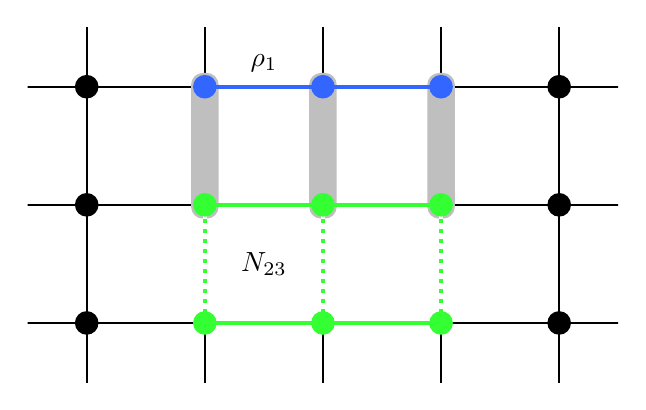
\begin{tikzpicture}[scale=0.5]
    % Define custom colors
\definecolor{customBlue}{rgb}{0.2, 0.4, 1}
\definecolor{customGreen}{rgb}{0.2, 1, 0.2}
\begin{scope}
\clip (-4.5,-1.5) rectangle (10.5,7.5);
\begin{scope}
    \foreach \x in {-6,-3,...,12} {
        \draw[thick, black] (\x,-3) -- (\x,9);
    }
    \foreach \y in {-3,0,...,9} {
        \draw[thick,black] (-6,\y) -- (12,\y);
    }
\end{scope}

    \fill[lightgray, rounded corners=0.15cm] (0-0.35,3+0-0.35) rectangle (0+0.35,6+0+0.35);
    \fill[lightgray, rounded corners=0.15cm] (3-0.35,3+0-0.35) rectangle (3+0.35,6+0+0.35);
    \fill[lightgray, rounded corners=0.15cm] (6-0.35,3+0-0.35) rectangle (6+0.35,6+0+0.35);

    \draw[customGreen, ultra thick] (0,0) -- (3,0) -- (6,0);  
    \draw[customGreen, ultra thick] (0,3) -- (3,3) -- (6,3);
    \draw[customBlue, ultra thick] (0,6) -- (3,6) -- (6,6);
    \draw[white, ultra thick] (0,0) -- (0,3);
    \draw[white, ultra thick] (3,0) -- (3,3);
    \draw[white, ultra thick] (6,0) -- (6,3);
    \draw[customGreen, ultra thick, dotted] (0,0) -- (0,3);
    \draw[customGreen, ultra thick, dotted] (3,0) -- (3,3);
    \draw[customGreen, ultra thick, dotted] (6,0) -- (6,3);


    \fill[black] (-3,0) circle (0.3);
    \fill[black] (-3,3) circle (0.3);
    \fill[black] (-3,6) circle (0.3);

    \fill[black] (9,0) circle (0.3);
    \fill[black] (9,3) circle (0.3);
    \fill[black] (9,6) circle (0.3);


    \fill[customGreen] (0,0) circle (0.3);
    \fill[customGreen] (3,0) circle (0.3);
    \fill[customGreen] (6,0) circle (0.3);

    \fill[customGreen] (0,3) circle (0.3);
    \fill[customGreen] (3,3) circle (0.3);
    \fill[customGreen] (6,3) circle (0.3);

    \fill[customBlue] (0,6) circle (0.3);
    \fill[customBlue] (3,6) circle (0.3);
    \fill[customBlue] (6,6) circle (0.3);

    \node[fill=white, inner sep=0pt] at (1.5,1.5) {$N_{23}$};
    \node at (1.5,6.6) {$\rho_1$};
\end{scope}
\end{tikzpicture}
}
\caption{ A tripartite graph state can be detected by preparing a network state, Bell measurements, and a fixed measurement. Entangled states of arrayed qubits can be detected by state preparation and a fixed measurement. }
\label{fig:chain}
\end{figure}

\begin{figure}
\centering
\resizebox{0.7\linewidth}{!}{
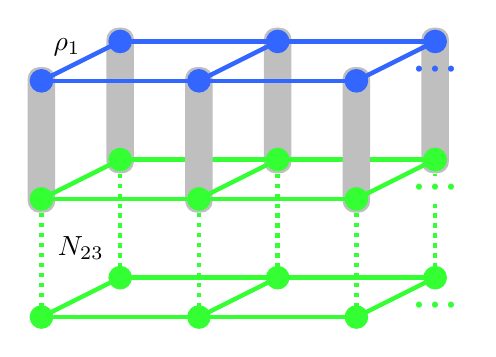
\begin{tikzpicture}[scale=0.5]
    % Define custom colors
    \definecolor{customBlue}{rgb}{0.2, 0.4, 1}
    \definecolor{customGreen}{rgb}{0.2, 1, 0.2}

    \fill[lightgray, rounded corners=0.15cm] (2-0.35,3+1-0.35) rectangle (2+0.35,6+1+0.35);
    \fill[lightgray, rounded corners=0.15cm] (6-0.35,3+1-0.35) rectangle (6+0.35,6+1+0.35);
    \fill[lightgray, rounded corners=0.15cm] (10-0.35,3+1-0.35) rectangle (10+0.35,6+1+0.35);

    \draw[customGreen, ultra thick] (0,0+0) -- (4,0+0) -- (8,0+0);  
    \draw[customGreen, ultra thick] (2,0+1) -- (6,0+1) -- (10,0+1); 
    \draw[customGreen, ultra thick] (0,0+0) -- (2,0+1);  
    \draw[customGreen, ultra thick] (4,0+0) -- (6,0+1);
    \draw[customGreen, ultra thick] (8,0+0) -- (10,0+1);

    \draw[customGreen, ultra thick] (2,3+1) -- (6,3+1) -- (10,3+1);

    \fill[lightgray, rounded corners=0.15cm] (0-0.35,3+0-0.35) rectangle (0+0.35,6+0+0.35);
    \fill[lightgray, rounded corners=0.15cm] (4-0.35,3+0-0.35) rectangle (4+0.35,6+0+0.35);
    \fill[lightgray, rounded corners=0.15cm] (8-0.35,3+0-0.35) rectangle (8+0.35,6+0+0.35);

    \draw[customGreen, ultra thick] (0,3+0) -- (4,3+0) -- (8,3+0);
    \draw[customGreen, ultra thick] (0,3+0) -- (2,3+1);
    \draw[customGreen, ultra thick] (4,3+0) -- (6,3+1);
    \draw[customGreen, ultra thick] (8,3+0) -- (10,3+1);
    
    \draw[customBlue, ultra thick] (0,6+0) -- (4,6+0) -- (8,6+0);
    \draw[customBlue, ultra thick] (2,6+1) -- (6,6+1) -- (10,6+1);
    \draw[customBlue, ultra thick] (0,6+0) -- (2,6+1);
    \draw[customBlue, ultra thick] (4,6+0) -- (6,6+1);
    \draw[customBlue, ultra thick] (8,6+0) -- (10,6+1);


    % First and second rows of disks
    \fill[customGreen] (0,0+0) circle (0.3);
    \fill[customGreen] (4,0+0) circle (0.3);
    \fill[customGreen] (8,0+0) circle (0.3);
    \fill[customGreen] (2,0+1) circle (0.3);
    \fill[customGreen] (6,0+1) circle (0.3);
    \fill[customGreen] (10,0+1) circle (0.3);

    \fill[customGreen] (0,3+0) circle (0.3);
    \fill[customGreen] (4,3+0) circle (0.3);
    \fill[customGreen] (8,3+0) circle (0.3);
    \fill[customGreen] (2,3+1) circle (0.3);
    \fill[customGreen] (6,3+1) circle (0.3);
    \fill[customGreen] (10,3+1) circle (0.3);

    \fill[customBlue] (0,6+0) circle (0.3);
    \fill[customBlue] (4,6+0) circle (0.3);
    \fill[customBlue] (8,6+0) circle (0.3);
    \fill[customBlue] (2,6+1) circle (0.3);
    \fill[customBlue] (6,6+1) circle (0.3);
    \fill[customBlue] (10,6+1) circle (0.3);

    \draw[customGreen, ultra thick, dotted] (0,0+0) -- (0,3+0);
    \draw[customGreen, ultra thick, dotted] (4,0+0) -- (4,3+0);
    \draw[customGreen, ultra thick, dotted] (8,0+0) -- (8,3+0);
    \draw[customGreen, ultra thick, dotted] (2,0+1) -- (2,3+1);
    \draw[customGreen, ultra thick, dotted] (6,0+1) -- (6,3+1);
    \draw[customGreen, ultra thick, dotted] (10,0+1) -- (10,3+1);

    \node at (10,0+0.25) [text=customGreen] {\huge \(\cdot\)\(\cdot\)\(\cdot\)};
    \node[fill=white, inner sep=0pt] at (10,3+0.25) [text=customGreen] {\huge \(\cdot\)\(\cdot\)\(\cdot\)};
    \node at (10,6+0.25) [text=customBlue] {\huge \(\cdot\)\(\cdot\)\(\cdot\)};

    \node[fill=white, inner sep=0pt] at (1,1.75) {$N_{23}$};
    \node at (0.65,6.85) {$\rho_1$};
\end{tikzpicture}
}
\caption{The estimation of entanglement witnesses for multipartite graph states.}
\label{graph state scheme}
\end{figure}

\subsection{ EWs for multipartite systems}

Thirdly, entanglement detection by state preparation can be extended to multipartite quantum states. We here, in particular, consider graph states, a class of states as a resource for MBQC \cite{PhysRevLett.86.5188}. Let us again present an instance for a three-qubit graph state, a Greenberger–Horne–Zeilinger (GHZ) state $|\psi\rangle = (|000\rangle +|111\rangle)/\sqrt{2}$ \cite{PhysRevA.62.062314}, see Fig. \ref{fig:chain}. An EW to detect a GHZ state may be given as,
\bea
W = \frac{1}{2} \mathbbm{1} - |\psi \rangle \langle \psi|.
\eea
A network state for an EW above can be constructed as,
\bea
N_{23} = \frac{1}{8} \sum_{a,b,c=0}^{1} \psi_{abc}^{(A_2 B_2 C_2)} \otimes \psi_{abc}^{(A_3 B_3 C_3)}.
\eea
where $\psi_{abc} = |\psi_{abc}\rangle \langle \psi_{abc}|$,
\bea
|\psi_{abc}\rangle = Z^a \otimes X^b \otimes X^c |\psi\rangle, ~~a,b,c \in \{0,1\}
\eea
with Pauli matrices $X$ and $Z$. It holds that
%\bea
%\tr[\rho W] =  8 \tr[\rho_1\otimes N_{23} P_{12} \otimes (\frac{\mathbbm{1}}{2} - |\psi \rangle\langle \psi |)_{3}], \nonumber
%\eea
\bea
{}_{A_3B_3C_3} \langle \psi |\rho_1 \otimes N_{23} ~P^{(12)} |\psi \rangle_{A_3B_3C_3} = \frac{1}{16} - \frac{1}{8}\tr[\rho W], \nonumber
\eea
which shows detection of a genuinely multipartite entangled state $\rho$ by finding that the left-hand-side is greater than $1/16$. Further generalization for detecting entangled $n$-qubit graph states is provided in Appendix. \\


\subsection{ To construct non-decomposable EWs }


Finally, let us investigate two entangled states defined by an EW. One denotes an entangled state $\rho_1$ detected by an EW, and the other $N_{23}$ realizing an EW by its preparation; see also Eq. (\ref{eq:ewm}). The result in Ref. \cite{PhysRevLett.96.150501} shows that an EW detects a set of entangled states that can activate its network state. Since a pair of PPT states cannot activate each other, either the states $\rho_1$ or $N_{23}$ must be non-PPT. Hence, a network state $N_{23}$ to detect a PPT entangled state $\rho_1$ should be non-PPT. We thus conclude that multipartite non-PPT entangled states can construct non-decomposable EWs, which are then highly non-trivial.
{
Note that non-PPT states can construct both decomposable and nondecomposable EWs, as shown in the example of reduction EWs, see Eq. \eqref{reductionEW}.
}
\\

{ \section{Robustness}
\label{sec:robust}

The framework for detecting entangled states in the subsection \ref{sec:gc} contains elements, the preparation of a network state and a fixed measurement for estimating a singlet fraction. We reiterate the relation between the estimation of an EW and the framework with a network state, 
\begin{align}
\tr[\rho W] = \alpha ~ \tr[\rho_1 \otimes N_{23} P^{(12)} (\eta \I - |\phi_{d}^+\rangle \langle \phi_{d}^+ | )_3 ],
\end{align}
for some $\alpha>0$. We here investigate the effect of noise on the preparation of a network state and a fixed measurement and show that the framework can unambiguously detect entangled states. That is, for separable states, the framework with noisy resources gives a non-negative expectation value. 


\begin{figure*}[t]
    \centering
    \includegraphics[scale=.18]{ fig4.pdf}
    \caption{  {Estimation of an EW in Eq. (\ref{eq:ewex}) can be realized in a circuit, where a network state in Eq. (\ref{eq:wr}) is realized and measurements in the computational basis are applied, see also Eq. (\ref{eq:ewr}). (1) A state for detecting entanglement, $|\psi^{-}\rangle$, is generated in registers $A_1B_1$. (2) A network state from an EW  is prepared to detect entanglement generated in $A_1B_1$. (3) A projection onto a state $|\phi^+\rangle $ is realized by collecting outcomes $00$ in registers $A_1A_2$. (4) A projection onto a state $|\phi^+\rangle $ is realized by collecting outcomes $00$ in registers $B_1B_2$. (5) Given outcomes $0000$ in registers $A_1B_1A_2B_2$, the singlet fraction is estimated in $A_3B_3$: a state in register $A_1B_1$ is entangled if the probability of outcomes $00$ in $A_3B_3$ is larger than $1/2$.  }}
    \label{fig:4}
\end{figure*}


\subsubsection*{ Noisy network states }
Suppose that the network states $N$ is noisy such that
\begin{align*}
\widetilde N &= (1-p) N + p \frac{\I}{d^{2n}},
\end{align*}
with some noise fraction $p$. It follows that,
\bea
&&\alpha~ \tr[\rho_1 \otimes \widetilde N_{23} P^{(12)} (\eta \I -  |\phi_{d}^+\rangle \langle \phi_{d}^+ | )_3 ] \nonumber \\
%&=&  \tr[\rho_1 \otimes ((1-p) N + p \frac{\I}{d^{2n}})_{23} P^{(12)} (\eta \I - \psi)_3 ]  \nonumber \\
&=& (1-p) \tr[\rho W] + \alpha p \frac{1}{d^{2n}} \frac{1}{d^{n}} (\eta d^n-1) \nonumber \\
&\geq & (1-p) \tr[\rho W]. \nonumber
\eea
Note that the term apart from $\tr[\rho W]$ in the second line is not negative since $\eta\leq 1/d$. Hence, noisy network states can be used to detect entangled states unambiguously. 



\subsubsection*{White noise in singlet fraction estimation}
Suppose that a fixed measurement setting for estimating a singlet fraction is noisy,
\begin{align}
(1-q)  |\phi_{d}^+\rangle \langle \phi_{d}^+ | + q \frac{\I}{d^n} \nonumber
\end{align}
with some noise fraction $q$. It follows that
\bea
&& \alpha ~ \tr[\rho_1 \otimes N_{23} P^{(12)} (\eta \I - (1-q)  |\phi_{d}^+\rangle \langle \phi_{d}^+ | - q \frac{\I}{d^n}  )_3 ]  \nonumber \\
 &= & (1-q)\tr[\rho W] + \alpha q \frac{1}{d^n} (\eta - \frac{1}{d^n} \tr[\rho^T N] ) \nonumber \\
 &\geq & (1-q) \tr[\rho W]. \nonumber
\eea
Thus, when a fixed measurement setting is noisy, the framework gives non-negative expectation values for separable states.

% \subsection{White noise in local Bell measurements}
% Now suppose that the local Bell measurements $P_{00}$ are replaced by  
% \begin{align*}
% \widetilde P = (1-r) P_{00} + r \frac{\I}{2^2}, % \label{noisy P}
% \end{align*}
% with the noise fraction $r$.
% With the noisy local Bell measurements, the state of interest $\rho$ is detected by MBEW if
% \begin{align}
% 0 &> \tr[\rho_1 \otimes N_{23} (\widetilde{P}\power{n})_{12} \otimes (\frac{1}{2}\I - \dyad{\vo}_G)^{(S'')}] \lb
% &= \tr \bigg[\rho_1 \otimes N_{23} (\frac{1}{2}\I - \dyad{\vo}_G)^{(S'')} \otimes \lb
% &\phantom{= \tr \bigg[} \left( \sum_{k=0}^{n} \binom{n}{k} q^{n-k} (\frac{1-q}{2^2})^k P_{00}\power{n-k} \otimes \I\power{k} \right)^{(SS')} \bigg] \lb
% &= \frac{1}{2^n} \tr \bigg[\rho_1 \otimes (\frac{1}{2}\I - \dyad{\vo}_G)^{(S')} \lb
% & \phantom{= \frac{1}{2^n} \tr\bigg[} \left( \sum_{k=0}^{n} \binom{n}{k} q^{n-k} (\frac{1-q}{2^2})^k P_{00}\power{n-k} \otimes \I\power{k} \right)^{(SS')} \bigg] \label{Bell noise exact}
% \end{align}
% It is too complicated to calculate exact value of the expression in the Ineq. (\ref{Bell noise exact}). Instead, let us consider an upper bound of the expression given by the worst case: the measurements are $P_{00}\power{n}$  (success) with a probability $q^n$, and $(\frac{\I}{2^2})\power n$ (fail) with a probability $1-q^n$. Then, the state $\rho$ is detected when
% \begin{align}
% \frac{1}{2^n} \left( q^n \frac{1}{2^n} \tr[\rho W] + (1-q^n) \frac{1}{2^{2n}} (\frac{1}{2} 2^n -1) \right) < 0,
% \end{align}
% which implies 
% \begin{align}
% \tr[\rho W] < (\frac{1}{2} - \frac{1}{2^n}) (1 - \frac{1}{q^n}).
% \end{align}
% }


\section{Realization in quantum circuits}


The framework of detecting entangled states by a fixed measurement can be realized in a quantum circuit. Here, we demonstrate the realization of a network state and the estimation of an EW with an example in Eq. (\ref{eq:ewex}). To facilitate the construction of a quantum circuit, we exploit a decomposition of the network state in the following, 
\begin{align}
N_{23} &= \frac{1}{4} \big( \ketbra{\psi^-}_{A_2 B_2} \otimes \ketbra{\phi^+}_{A_3 B_3}  \nonumber \\
&~~~~~~ + \ketbra{\psi^+}_{A_2 B_2} \otimes \ketbra{\psi^+}_{A_3 B_3} \nonumber \\
&~~~~~~ + \ketbra{\phi^-}_{A_2 B_2} \otimes \ketbra{\phi^-}_{A_3 B_3} \nonumber \\
&~~~~~~ + \ketbra{\phi^+}_{A_2 B_2} \otimes \ketbra{\psi-}_{A_3 B_3} \big), 
\end{align}
which is identical to the state in Eq. \eqref{eq:wr}. Then, a circuit for realizing the network state is shown in Fig. \ref{fig:4}, where blocks (1)-(5) describe realizations of a network state, projection on a state $|\phi^+\rangle$, measurements of estimating the singlet fraction. We remark that a fixed measurement setting is used for estimating an EW. 

Considering the effect of noise in Section \ref{sec:robust}, one may expect that the framework can be realized in a noisy implementation of quantum information processing. We then implemented the circuit in the IBMQ Kyiv on April 2, 2025. The results are presented in Fig. \ref{fig:result}, demonstrating the robustness of the proposed framework for estimating EWs in a realistic setting. Although noise is present, the estimation of an EW shows a singlet fraction $0.61$ higher than the threshold $1/2$, detecting the presence of an entangled state in registers $A_1B_1$.


%\begin{figure}[t]
%\centering
%\[
%\Qcircuit @C=1em @R=.7em @!R {
%\lstick{A_1} & \gate{H} & \ctrl{1} & \gate{Z} & \qw        & \qw        & \ctrl{2} & \gate{H} & \qw      & \qw      & \meter & \cw \\
%\lstick{B_1} & \qw      & \targ    & \gate{X} & \qw        & \qw        & \qw      & \qw      & \ctrl{2} & \gate{H} & \meter & \cw \\
%\lstick{A_2} & \gate{H} & \ctrl{1} & \gate{Z} & \qw        & \qw        & \targ    & \qw      & \qw      & \qw      & \meter & \cw \\
%\lstick{B_2} & \qw      & \targ    & \gate{X} & \targ      & \ctrl{0}   & \qw      & \qw      & \targ    & \qw      & \meter & \cw \\
%\lstick{A_3} & \gate{H} & \qw      & \qw      & \ctrl{-1}  & \qw        & \gate{H} & \ctrl{1} & \ctrl{1} & \gate{H} & \meter & \cw \\
%\lstick{B_3} & \gate{H} & \qw      & \qw      & \qw        & \ctrl{-2}  & \qw      & \targ    & \targ    & \qw      & \meter & \cw \\
%}
%\]
%    \caption{ The quantum circuit for detection of $\ket{\psi^-}_{A_1 B_1}$ using a pure network state $\ket{N}_{A_2B_2A_3B_3}$, which implements the EW $W = \tfrac{1}{2} \I - \psi^-$ \eqref{eq:ewex}. The first three layers in $A_1 B_1$ generate $\ket{\psi^-}$ state, while first five layers within $A_2 B_2 A_3 B_3$ generate $N$. The CNOT gates followed by $H$ gate and measurements in $A_1 A_2$ and $B_1 B_2$ implements local Bell projections. The measuremnet outcome $0000$ for the first four bits corresponds to the $\phi^+$ projections on both sides.}
 %   \label{fig:flip EW circuit}
%\end{figure}

\begin{figure}[t]
    \centering
    \includegraphics[scale=.13]{ fig5.pdf}
    \caption{ { The circuit in \ref{fig:4} is run in the IBMQ Kyiv. Given outcomes $0000$ in registers $A_1A_2B_1B_2$, the singlet fraction in registers $A_3B_3$ corresponds to the probability of having an outcome $00$. While $10000$ counts are obtained for registers $A_1A_2A_3B_1B_2B_3$, we have $685$ counts for $0000$ on $A_1A_2B_1B_2$, given which we have the singlet fraction $0.61$ which is larger than $1/2$. While the IBMQ Kyiv is noisy, we have demonstrated the generation and the detection of entangled states on a quantum circuit. 
    }}
    \label{fig:result}
\end{figure}

\section{Conclusion}


In conclusion, we have established an MB framework for estimating observables, in particular EWs, and shown the construction of network states for observables. It is also of fundamental interest to find that entanglement demonstrates elements of quantum theory, both dynamics, i.e., MBQC and observables. Our results shed new light on detecting and manipulating entangled states in a realistic scenario where precise controls via quantum gates are yet limited, such as an array of superconducting qubits, neutral atoms, or photons, where the preparation of a multipartite state and a fixed measurement are readily experimentally feasible. The results also open a new avenue of exploiting entangled states in distributed quantum information processing such as computing and metrology where entanglement is resourceful and quantum estimation {\it per se} corresponds to computing or metrology. 

In future directions, it would be interesting to realize the estimation of EWs via network states experimentally by considering the effects of noise in a realistic setting. Note that some network states, such as Smolin, have been realized in experiment \cite{Amselem:2009aa, PhysRevLett.105.130501, PhysRevLett.109.040501}. It is also interesting to exploit network states in a network and security scenario such as a measurement-device-independent scenario, see Refs. \cite{PhysRevLett.108.200401,PhysRevLett.110.060405}, so that observables such as EWs are estimated by relaxing assumptions on joint measurements; estimation of EWs, as well as detection of entanglement, is achieved in a higher level of robustness against imperfect implementations. 

\section*{Acknowledgement}

This work is supported by National Research Foundation of Korea (NRF-2021R1A2C2006309, NRF-2022M1A3C2069728) and the Institute for Information \& Communication Technology Promotion (IITP) (RS-2023-00229524, the ITRC Program/IITP-2023-2018-0-01402). AB and DC were supported by the Polish National Science Center project No. 2018/30/A/ST2/00837.


\bibliographystyle{quantum}
% \bibliography{bibedsp}
\input{qde.bbl}

\onecolumn
\appendix

\section*{Appendix}

\section{Entanglement detection by state preparation for two-qubit states}
\label{app1}

We here reproduce a duplex state for two-qubit EWs. Let $|\phi^{\pm}\rangle = (|00\rangle\pm |11\rangle )/\sqrt{2}$ and $|\psi^{\pm}\rangle = (|01\rangle\pm |10\rangle )/\sqrt{2}$ denote four Bell states. We show how to construct a duplex state for an EW 
\bea
W = |\phi^+\rangle \langle \phi^+|^{\Gamma} = \frac{1}{2}\mathbbm{I} - |\psi^-\rangle \langle \psi^-|. \nonumber
\eea
One may find a decomposition of the above EW in the following way
\bea
W = \frac{1}{2} (\mathbbm{I} -  |\psi^-\rangle \langle \psi^-|) -\frac{1}{2} |\psi^-\rangle \langle \psi^-|, \nonumber
\eea
where two non-negative operators are obtained as $ |\psi^-\rangle \langle \psi^-|$ and $(\mathbbm{I} -  |\psi^-\rangle \langle \psi^-|)/2$. A duplex state may be written as
\bea
N_{23} &=& c_1 |\psi^-\rangle_{A_2 B_2 } \langle \psi^-| \otimes \Pi_{A_3B_3}(1) + \nonumber\\
&& \frac{c_2}{3} (\mathbbm{I} - |\psi^-\rangle_{A_2 B_2 } \langle \psi^-| ) \otimes \Pi_{A_3B_3}(2), \nonumber
\eea
for some positive constants $c_1,~c_2=1-c_1>0$ and non-negative normalized operators $\Pi(1),~ \Pi(2)\geq 0$. To realize entanglement detection of a state of interest $\rho$ using an entanglement witness $W$, one may seek $N_{23}$ that satisfy 
\bea
\tr[\rho_1 W_1] =  16~ \tr  [\rho_1\otimes N_{23} (\eta \mathbbm{1} - | \phi^+\rangle_{A_3B_3} \langle \phi^+|) \otimes P^{(12)}  ], \nonumber 
\eea
with $\eta = 1/2$, since all two-qubit entangled states are distillable. The goal is now to find the parameters $c_1,~c_2,~ \Pi(1)$ and $\Pi(2)$ that satisfy the relation in the above. The left-hand-side (lhs) is given by
\bea
\mathrm{lhs}= \frac{1}{2} - \langle \psi^-| \rho|\psi^-\rangle, \nonumber
\eea
and the right-hand-side (rhs) by
\bea 
\mathrm{rhs}&=& 2 \tr [\rho_{2}^T N_{23}] - 4 \tr [\rho_{2}^T \otimes |\psi^-\rangle \langle \psi^-|  N_{23} ]    \nonumber \\
&=& c_2( \frac{2}{3}  - \frac{4}{3} \langle \phi^+| \Pi (2) |\phi^+\rangle )  + L \langle \psi^-| \rho |\psi^-\rangle, \nonumber
\eea
where 
\bea
L &=& c_1 (2-4 \langle \phi^+| \Pi(1) | \phi^+\rangle ) +  \nonumber \\
 && c_2 ( - \frac{2}{3}  + \frac{4}{3} \langle \phi^+| \Pi(2) | \phi^+\rangle ). \nonumber
\eea
From the lhs and the rhs, one can find that
\bea
c_2( \frac{2}{3}  - \frac{4}{3} \langle \phi^+| \Pi (1) |\phi^+\rangle )= \frac{1}{2}~\mathrm{and} ~L=-1, \nonumber
\eea
from which 
\bea
&& c_1 (2-4 \langle \phi^+| \Pi(1) | \phi^+\rangle ) = - \frac{1}{2} \nonumber\\
& \iff &c_1 = \frac{1}{8 \langle \phi^+ | \Pi(1) |\phi^+\rangle -4 } >0. \nonumber
\eea
For convenience, we choose $\Pi(1) = |\phi^+\rangle \langle \phi^+|$ although it is not a unique choice. It follows that $c_1=1/4$ and $c_2=3/4$. The consequence is that $\langle \phi^+| \Pi(2) |\phi^+\rangle = 0$. Thus, we have 
\bea
\Pi(2) = \frac{1}{3} ( \mathbbm{I} -|\phi^+\rangle \langle \phi^+| ).\nonumber
\eea
All these conclude a duplex state
\bea
N_{23} &=& \frac{1}{4} |\psi^-\rangle_{A_2B_2} \langle \psi^-| \otimes |\phi^+\rangle_{A_3B_3} \langle \phi^+| + \nonumber \\
&&\frac{1}{12} (\mathbbm{1} - |\psi^-\rangle_{A_2B_2} \langle \psi^-|) \otimes (\mathbbm{1} - |\phi^+\rangle_{A_3B_3} \langle \phi^+|). \nonumber
\eea
Note that a duplex state for an EW is not unique. 


\section{Duplex states for high-dimensional EWs}
\label{app2}

\subsection{The framework}

Recall that for a given EW $W$, we are looking for a duplex state $N_{23} = N^{(A_2 B_2 A_3 B_3)}$, which are separable in $A_2 B_2: A_3 B_3$, satisfying the following condition:
\bea
W_2^T \propto \tr_3[N_{23} (\eta \mathbbm{1} - P_{00})_3], 
\eea
for some $\eta \in [\frac{1}{d}, 1)$.
It is easy to see that the following relation holds:
\bea
\tr[\rho_1 W_1] &=& d^2 \tr[\rho_1 \otimes W_2^T P^{(12)}]
\\ &\propto& \tr[\rho_1 \otimes N_{23} ~ P^{(12)} \otimes (\eta \mathbbm{1} - P_{00})_3], \label{prop}
\eea
where $P^{(12)} = P_{00}^{(A_1 A_2)} \otimes P_{00}^{(B_1 B_2)}$ denotes the Bell measurements on both sides.
The scheme can be understood as follows. First, a filtering operation $\Lambda^{(1 \to 3)}$ teleports the state $\rho_1$ to $A_3 B_3$, leaving a result state $\Lambda(\rho)$:
\bea
\Lambda^{(1 \to 3)} (\rho) = \frac{\tr_{12}[\rho_1 \otimes N_{23} P^{(12)}] }{\tr[\rho_1 \otimes N_{23} P^{(12)}] }. \label{filtering}
\eea
Then the singlet fraction, or the overlap with the Bell state $P_{00}$, of the resulting state $\Lambda(\rho)$ is checked whether it is higher than $\eta$ or not. 

The singlet fraction can also be estimated with a fixed measurement on individual quantum systems. The main idea is to place unitary interactions before a measurement. A $d$-dimensional Hadamard gate and a $d$-dimensional CNOT gate may be obtained as,
\begin{align*}
H &= \sum_{j,k=0}^{d-1} e^{2 \pi ijk/d} \ket{j}\bra{k},~ \mathrm{and}
\\ U_{CNOT} &= \sum_{j=0}^{d-1} \ket{j}\bra{j} \otimes \sum_{k=0}^{d-1} \ket{k+j}\bra{k}.    
\end{align*}
Note that a maximally entangled state can be generated,  $\ket{\phi_{00}} = U_{CNOT}(H \otimes \I) \ket{00}$. Then, instead of a joint measurement, one can first apply $(H^\dagger \otimes \I) U_{CNOT}^\dagger $ to a resulting state $\Lambda^{(1 \to 3)} (\rho)$ and then perform a measurement in the computational basis. The probability of having outcomes $00$ gives the singlet fraction $\langle \phi_{00} | \Lambda(\rho) | \phi_{00} \rangle$.
It holds that $\langle \phi_{00} | \Lambda(\rho) | \phi_{00} \rangle > \eta$ if and only if $\tr[\rho W] < 0$, which certifies that a state $\rho$ given in the beginning is entangled. \\

\subsection{ Decomposable EW}

Consider a decomposable EW $W = Q^\Gamma$ for $Q\geq 0$ and $\tr[Q]=1$. Let $\lambda:=\max_{i}|\lambda_i|$ where $\{\lambda_i\} $ are eigenvalues of $W$. Then, a duplex state for the EW is obtained as
\bea
N_{23}^{\text{(dec)}} &=& c_1\left( \frac{\lambda\mathbbm{1} - Q^\Gamma }{\lambda d^2 - 1 }\right)^{(2)} \otimes P_{00}^{(3)} \nonumber\\
&&+ c_2 \left( \frac{ \lambda \mathbbm{1} +  Q^{\Gamma} }{\lambda d^2 + 1}\right)^{(2)} \otimes \left( \frac{\mathbbm{1} - P_{00}}{d^2 - 1}\right)^{(3)},~~ \label{decom NS}
\eea
with the threshold value $\eta = \frac{1}{d}$, 
\bea
c_1 = \frac{d^2 \lambda - 1}{d^3 \lambda  + d -2} ~~\mathrm{and}~ ~ c_2= \frac{(d-1)(d^2 \lambda +1)}{d^3 \lambda  +d-2}. \nonumber
\eea
The superscript $(j)$ stands for the composite space $A_j B_j$ for $j \in \{1,2,3\}$.
From the equation
\bea
\tr_3[ N_{23 } (\frac{1}{d}\mathbbm{1}-P_{00})_3] = \frac{2(d-1)}{d(d^3 \lambda + d -2)} Q^\Gamma, \nonumber
\eea
it holds that
\bea
& \tr[\rho W] = k ~ \tr[\rho_1 \otimes N_{23} ~ P^{(12)} \otimes (\frac{1}{d}\mathbbm{1}-P_{00})_3], & \nonumber
\\ & \bracket{\phi_{00}}{\Lambda(\rho)}{\phi_{00}} > \frac{1}{d }\iff \tr[\rho W] <0, &
\eea
where $k=\frac{d(d^3 \lambda + d -2)}{2(d-1)}$.

Hence, the partial transpose criteria can be realized by preparing a duplex state in Eq. (\ref{decom NS}). In particular, a duplex state for the decomposable EW 
\bea
W = P_{00}^{\Gamma} = \frac{\mathbbm{F}}{d},
\eea
which is proportional to the flip operator $\mathbbm{F}$ that detects entangled Werner states, can be found as 
\bea
N_{23}^{\text{(flip)}} &=& \frac{1}{d+2} \left( \frac{\mathbbm{1}-\mathbbm{F}}{d^2-d} \right)^{(2)} \otimes P_{00}^{(3)}  \nonumber
\\ && + \frac{d+1}{d+2} \left( \frac{\mathbbm{1}+\mathbbm{F}}{d^2+d} \right)^{(2)} \otimes \left( \frac{\mathbbm{1}-P_{00}}{d^2-1} \right)^{(3)}.~~ \label{flip NS}
\eea
Note that this duplex state is invariant under $U_{A_2} \otimes U_{B_2} \otimes V_{A_3} \otimes V^*_{B_3}$ for any unitary operation $U, V$. This duplex state is positive under the partial transpose $A_2 A_3: B_2 B_3$, so it is undistillable. This state (\ref{flip NS}) has been used in the activation of non-PPT entangled states and proved to be PPT in \cite{PhysRevLett.88.247901}.

\subsection{ Bell-diagonal EW}
The next examples are Bell-diagonal witnesses $W(\Vec{\lambda})$, which are decomposable or non-decomposable depending on the parameter $\Vec{\lambda} = (\lambda_0, \ldots, \lambda_{d-1})$:
\bea
W(\Vec{\lambda}) = \sum_{s=0}^{d-1} \lambda_s \Pi_s - P_{00}, \label{eq:Wa2}
\eea
where $\lambda_s \ge 0 ~\forall s$ and $\sum_{s=0}^{d-1} \lambda_s = 1$. 
Note also that $W[\Vec{\lambda}]$ in Eq. (\ref{eq:Wa2}) is an EW if a vector $\Vec{\lambda}$ satisfies the cyclic inequalities in the following, 
\bea
\sum_{j=0}^{d-1} \frac{t_{j}^2}{\sum_{s=0}^{d-1} \lambda_s t_{j+s}^2} \le d, \nonumber
\eea
for all $t_0, \ldots, t_d \ge 0$.
The value $\lambda_0$ is critical in implementing this witness with state preparation, as shown below. To construct a duplex state for a Bell-diagonal EW, we use paired Bell-diagonal (PBD) states:
\bea
N_{23}^{\textrm{(PBD)}} (\Vec{\lambda}) = \sum_{s=0}^{d-1} \lambda_s \frac{1}{d} \sum_{t=0}^{d-1} P_{st}^{(2)} \otimes P_{st}^{(3)},
\eea
with the threshold value $\eta = \lambda_0$. 
Then the following holds:
%\bea
%& \tr_3[ N_{23}^{\textrm{(PBD)}} (\lambda_0 \mathbbm{1} - P_{00})_3 ] = \frac{\lambda_0}{d} W_2^T (\Vec{\lambda}), & \nonumber
%\eea
\bea
& \tr[\rho W(\Vec{\lambda})] = k ~\tr[\rho_1 \otimes N_{23}^{\textrm{(PBD)}}(\Vec{\lambda})~ P^{(12)} \otimes (\lambda_0 \mathbbm{1} - P_{00})_3 ], & \nonumber
\\ & \bracket{\phi_{00}}{\Lambda(\rho)}{\phi_{00}} > \lambda_0 \iff \tr[\rho W(\Vec{\lambda})] <0. \nonumber &
\eea
where $k = d^3 / \lambda_0$. It is possible to achieve $\bracket{\phi_{00}}{\Lambda(\sigma)}{\phi_{00}} = \lambda_0$ with a separable state $\sigma$:
\bea
\Lambda^{(1 \to 3)} (\sigma) &=& \frac{\tr_{12}[\sigma_1 \otimes N_{23} P^{(12)}] }{\tr[\sigma_1 \otimes N_{23} P^{(12)}] }, \nonumber
\\ \textrm{where } \sigma &=& \frac{1}{d} P_{00} + \frac{1}{d} \sum_{s=1}^{d-1} \frac{\Pi_s}{d}. \nonumber
\eea
In particular, EWs from a reduction map and  the Choi map can be written in the form of Bell-diagonal witness and can be implemented by preparing the corresponding PBD state.
A decomposable EW from the reduction map corresponds to a Bell-diagonal EW with $\Vec{\lambda} = (\frac{1}{d}, \ldots, \frac{1}{d})$:
\bea
W_{\textrm{red}} &=& \sum_{s=0}^{d-1} \frac{1}{d} \Pi_s - P_{00} = \frac{1}{d} \mathbbm{1} - P_{00} \label{red},
\\ N_{23}^{\textrm{(red)}} &=& \frac{1}{d^2} \sum_{s=0}^{d-1} \sum_{t=0}^{d-1} P_{st}^{(2)} \otimes P_{st}^{(3)},
\eea
with the threshold value $\eta = \frac{1}{d}$.

The PBD state $N_{23}^{\textrm{(red)}}$ can be seen as a direct generalization of Smolin state \cite{PhysRevA.63.032306} into $d$-dimension. In $d=2$, Smolin state is PPT in $A_2 A_3:B_2 B_3$. However, the state $N_{23}^{\textrm{(red)}}$ is not PPT in higher dimensions $d \ge 3$ in general. Smolin state in two-dimension is undistillable, but the distillability of $N_{23}^{\textrm{(red)}}$ in higher dimensions is unknown.

Although it can be generalized into higher dimensions \cite{PhysRevA.84.024302, doi:10.1142/S1230161213500066}, the nondecomposable witness from Choi map \cite{Choi:1975aa} is defined in $d=3$ and corresponds to a Bell-diagonal witness with $\Vec{\lambda} = (\frac{2}{3}, \frac{1}{3}, 0)$:
\bea
W_{\textrm{Choi}} &=& \frac{2}{3} \Pi_0 + \frac{1}{3} \Pi_1 - P_{00},
\\ N_{23}^{\textrm{(Choi)}} &=& \frac{2}{9} \sum_{t=0}^{2} P_{0,t}^{(2)} \otimes P_{0,t}^{(3)} + \frac{1}{9} \sum_{t=0}^{2} P_{1,t}^{(2)} \otimes P_{1,t}^{(3)},~~~~~~
\eea
with the threshold value $\eta = \frac{2}{3}$.


\subsection{  Breuer-Hall EW}

The Breuer-Hall map \cite{PhysRevLett.97.080501, Hall_2006} finds an EW,
\bea
W_{\textrm{BH}} = \frac{1}{d} (\mathbbm{1}- \mathbbm{F}') - P_{00} ,
\eea
where $\mathbbm{F}' = (\mathbbm{1} \otimes U) \mathbbm{F} (\mathbbm{1} \otimes U^\dagger)$ for any skew-symmetric unitary operator $U$ such that $UU^\dagger = \mathbbm{1}$ and $U^T = -U$. In even dimensions $d=2n$, one can set $U$ as
\bea
U = \Oplus_{i=1}^{n} 
\begin{bmatrix}
0 & 1 \\
-1 & 0 
\end{bmatrix}, \nonumber
\eea
then it acts as $U \ket{i} = (-1)^{j} \ket{j}$ where $j = i+1$ for even $i$ and $j = i-1$ for odd $i$.

One can think of $W_{\textrm{BH}}$ as a combination of reduction EW (\ref{red}) and the flip operator from reduction map with additional $U$.
A duplex state for the BH EW is as follows,
\bea
N_{23}^{(\textrm{BH})}  %& = & c_0 N^{(23)}_{\textrm{PBD}} + (1-c_0) N^{(23)}_{\textrm{skew}}, \label{eq:bhn} \\
& = & c_0 \frac{1}{d^2} \sum_{s=0}^{d-1} \sum_{t=0}^{d-1} P_{st}^{(2)}  \otimes P_{st}^{(3)} \nonumber \\
&& + c_1 \left( \frac{\mathbbm{1} + \mathbbm{F}' }{d^2+d} \right)^{(2)} \otimes P_{00}^{(3)}   \nonumber \\
&& + c_2 \left( \frac{\mathbbm{1} - \mathbbm{F}' }{d^2-d} \right)^{(2)} \otimes \left( \frac{\mathbbm{1} - P_{00}}{d^2-1} \right)^{(3)},~~~~ \label{eq:nbh} 
\eea
with the threshold value $\eta = \frac{1}{d}$, where $c_0 = \frac{2d^2-2d}{3d^2 -3d +2}$, $c_1= \frac{d+1}{3d^2-3d+2}$, and $c_2 = \frac{d^2-2d+1}{3d^2-3d+2}$. One can show that
\bea
 \tr_3[ N_{23}^{(\mathrm{BH})}~ (\eta \mathbbm{1} - P_{00})_3] = \frac{c_0}{d^2} W_{\mathrm{BH}}^T,
\eea
which leads to
\bea
& \tr[\rho W_{\textrm{BH}}] = k ~\tr[\rho_1 \otimes N_{23}^{\textrm{(BH)}}~ P^{(12)} \otimes (\eta \mathbbm{1} - P_{00})_3 ], & \nonumber
\\ & \bracket{\phi_{00}}{\Lambda(\rho)}{\phi_{00}} > \frac{1}{d} \iff \tr[\rho W_{\textrm{BH}}] <0, \nonumber &
\eea
where $k =  d^4 / c_0$.

%There is a final remark on the relation between the duplex state $N_{23}$ and the corresponding EW $W$. If the state $N_{23}$ is PPT under $A_2A_3:B_2B_3$, then the EW $W$ must be decomposable, and the threshold value is $\eta=\frac{1}{d}$. This can be understood as a view of activating distillability. Suppose that both states $\rho_1$ and $N_{23}$ are PPT, so undistillable. They remain PPT after the local projections $P_{00}^{(A_1 A_2)} \otimes P_{00}^{(B_1 B_2)}$, so the upper bound of the singlet fraction of $\Lambda(\rho)$ is $\frac{1}{d}$. For some state $\tau$, $\Lambda(\tau)$ having a singlet fraction higher than $\frac{1}{d}$ implies that $\tau_1 \otimes N_{23}$ is distillable \cite{PhysRevA.59.4206}, which implies that $\tau$ is non-PPT. The EW constructed from a PPT duplex state cannot detect PPT entangled states, i.e., it is decomposable.
%The contraposition states that to make a nondecomposable EW, the duplex state must be non-PPT. However, the converse does not hold: an EW constructed from a non-PPT duplex state is not always nondecomposable. A counterexample is already given in the paper: the reduction witness is decomposable in any dimension, while high-dimensional Smolin states are non-PPT. The relations between other properties of EW, e.g., atomicity and optimality, and the properties of duplex states remain open questions.



\begin{figure}[t]
\centering
\includegraphics[width=8.8cm ]{figm}
\caption{ A graph state can be detected by preparing a duplex state, Bell measurements, and a fixed measurement. }
\label{fig:figm}
\end{figure}




\section{Entanglement witnesses for graph states}
\label{app3}
A graph $G = (V ,E)$ is defined by a set of vertices $V$ and a set of edges $E$:
\bea
V &=& \{1,\ldots,n\}, ~ \text{where $n$ is the number of vertices,} \nonumber
\\ E &=& \{(i,j)| i,j \in V, i<j, \text{Vertex $i$ and $j$ are connected.}\} \nonumber
\eea
Also define the neighborhood of vertex $i$: $E_i = \{j \in V| (i,j) \in E \text{ or } (j,i) \in E\}$, which is a set of vertices connected to vertex $i$.
% A graph $G = (V ,E)$ is defined by a set $V$ of vertices corresponding to qubits and a set $E = (E_1, \ldots, E_n)$ of edges connecting some of these vertices, where $E_i$ is the set of vertices connected to the $i$-th vertex.

The generators $g_i$ and the projectors $\gamma_i$ of a graph state determined by the graph $G$ are given by
\bea
g_i &=& X_i \prod_{j \in E_i} Z_j, \nonumber
\\ \gamma_i^{(x_i)} &=& \frac{\mathbbm{1}+(-1)^{x_i} g_i}{2}.
\eea
Note that the eigenvalue of $g_i$ is either 1 or -1, and the eigenvalue of $\gamma_i$ is either 1 or 0. Now we define an orthonormal graph state basis consisting of $2^n$ states:
\bea
\ket{\Vec{x}}\bra{\Vec{x}}_G = \prod_{i=1}^{n} \gamma_i^{(x_i)}, ~~ \text{where } \Vec{x} = (x_1, \ldots, x_n) \in \{0,1\}^n. \nonumber
\eea
The states $\ket{\Vec{x}}_G$ are the eigenstates of the generators and projectors: 
\bea
g_i \ket{\Vec{x}}_G &=& (-1)^{x_i} \ket{\Vec{x}}_G, \\
\gamma_i^{(k)} \ket{\Vec{x}}_G &=&
\begin{cases}
\ket{\Vec{x}}_G & \mbox{if}\; x_i = k,\\
0 & \mbox{if}\; x_i \ne k.
\end{cases}
\eea
A graph state, denoted by $\ket{\Vec{0}}\bra{\Vec{0}}_G$, corresponds to an eigenstate with eigenvalue $+1$ for all generators $g_i$ ($i \in \{1, \ldots, n\}$). A state can be obtained by preparing $\ket{+} = (\ket{0}+\ket{1})/\sqrt{2}$ placed at vertices in $V$, and applying the controlled-Z ($CZ$) gate to all edges in $E$, see Fig. \ref{fig:graph}.

\begin{figure}[t]
\centering
\includegraphics[width=7cm]{cluster.pdf}
\caption{A graph consisting of a set of vertices and a set of edges uniquely defines the graph state. The graph state can be obtained by preparing $\ket{+} = (\ket{0}+\ket{1})/\sqrt{2}$ at all vertices in $V$, and applying the controlled-Z ($CZ$) gats to all edges in $E$.}
\label{fig:graph}
\end{figure}

\begin{figure}[t]
\centering
\includegraphics[width=8cm]{Cl4.pdf}
\caption{The four-qubit linear cluster state on the graph $G_{Cl4}$. One can obatin the graph state $\ketbra{0000}_G$ by preparing four $\ket{+}$ states and applying the controlled-Z gate to three edges.}
\label{fig:Cl4}
\end{figure}

For instance, the four-qubit linear cluster state can be defined by a graph $G_{Cl4} = (V_4,E_{Cl4})$, where $V_4 = \{1,2,3,4\}$ and $E_{Cl4} = \{(1,2),(2,3),(3,4)\}$, see Fig. \ref{fig:Cl4}. 
% The neighborhood of vertices are given by $E_1=\{2\}$, $E_2=\{1,3\}$, $E_3=\{2,4\}$, $E_4=\{3\}$. 
The generators define $16$ graph states $\ket{0000}\bra{0000}_G, \ldots,$ and $\ket{1111}\bra{1111}_G$. The graph state $\ket{0000}\bra{0000}_G$ is detected by an EW in the following,
\bea
W_{Cl4} = \frac{1}{2} \sum_{\Vec{x} \in S} \ket{\Vec{x}}\bra{\Vec{x}}_G - \ketbra{0000}_G,
\eea
where $S = \{$0000, 0001, 0010, 0011, 0100, 0101, 0110, 0111, 1000, 1010, 1100, 1110$\}$. Then the duplex state for this graph state can be constructed by 
\bea
N_{23}^{(Cl4)} = \sum_{\Vec{x} \in S} \frac{1}{12} \ketbra{\Vec{x}}_G^{(2)} \otimes \ketbra{\Vec{x}}_G^{(3)}.
\eea
It holds that
\bea
&& \tr[\rho_1 \otimes N_{23}^{(Cl4)} P^{(12)} \otimes ( \frac{1}{2}\mathbbm{1} - \ketbra{0000}_G ) ] \nonumber
\\ && \propto \tr[\rho W_{Cl4}],
\eea
where
\bea
P^{(12 )} &=& |\phi^{+}\rangle_{A_1A_2}\langle \phi^+| \otimes |\phi^{+}\rangle_{B_1B_2}\langle \phi^+| \nonumber
\\ && \otimes |\phi^{+}\rangle_{C_1C_2}\langle \phi^+| \otimes |\phi^{+}\rangle_{D_1D_2}\langle \phi^+|. \nonumber
\eea
Then a four-qubit entangled state $\rho$ is detected by $W_{Cl4}$ when
\bea
{}_{G} \langle 0000| \Lambda [\rho]| 0000\rangle_G > \frac{1}{2},
\eea
where the map $\Lambda^{(1 \to 3)}$ is defined as,
\bea
\Lambda^{( 1\rightarrow 3)} [\rho]= \frac{ \tr_{12}[\rho_{1}\otimes N_{23} P^{(12)}] }{ \tr[\rho_1\otimes N_{23} P^{(12)}]  }. \nonumber
\eea
\\

A typical decomposable EW can be written in the following form \cite{PhysRevA.84.032310}:
\bea
W_G = \frac{1}{2} \sum_{\Vec{x} \in S} \ketbra{\Vec{x}}_G - \ketbra{\Vec{0}}_G,
\eea
where the set $S \subseteq \{0,1\}^n$ depends on $W_G$.
Then the duplex states $N_{23}^{G}$ for this entanglement witnesses are given by
\bea
N_{23}^{(G)} = \sum_{\Vec{x} \in S} \frac{1}{|S|} \ketbra{\Vec{x}}_G^{(2)} \otimes \ketbra{\Vec{x}}_G^{(3)}.
\eea
An $n$-qubit entangled state $\rho$ is detected by $W_G$ when
\bea
{}_{G} \langle \Vec{0}| \Lambda [\rho]| \Vec{0}\rangle_G &>& \frac{1}{2},
\eea
for
\bea
\Lambda^{( 1\rightarrow 3)} [\rho] &=& \frac{ \tr_{12}[\rho_{1}\otimes N_{23} P^{(12)}] }{ \tr[\rho_1\otimes N_{23} P^{(12)}]  }, \nonumber\\ 
P^{(12)} &=& \Otimes_{v \in V} |\phi^+\rangle_{v_1 v_2}\langle\phi^+|, \nonumber
\eea
where $V$ denotes the set of vertices of the graph $G$. 

% Then the overlap with the graph state $\ket{\Vec{0}}_G$ of the result state $\Lambda[\rho]$ is checked whether it is higher than $\frac{1}{2}$ or not. 
The overlap ${}_{G} \langle \Vec{0}| \Lambda [\rho]| \Vec{0}\rangle_G$ can be estimated with a fixed measurement on individual qubits. Note that a graph state is generated as follows, $\ket{\Vec{0}}_G$ is obtained as $\ket{\Vec{0}}_G = (\Otimes_{e \in E} U_{CZ}) (\Otimes_{v \in V} H) \ket{0}^{\otimes n}$. Then, the estimation of a singlet fraction can be achieved by applying an interaction $(\Otimes_{v \in V} H) (\Otimes_{e \in E} U_{CZ})$ to a resulting state $\Lambda^{(1 \to 3)} [\rho]$ and then performing a measurement in the computational basis.  The probability of obtaining an outcome $00$ gives the overlap ${}_{G} \langle \Vec{0}| \Lambda [\rho]| \Vec{0}\rangle_G$.
It holds that ${}_{G} \langle \Vec{0}| \Lambda [\rho]| \Vec{0}\rangle_G > \frac{1}{2}$ if and only if $\tr[\rho W] < 0$, which certifies that $\rho$ is entangled.

\end{document}

\onecolumn
\appendix

\section*{Appendix}

\section{Entanglement detection by state preparation for two-qubit states}
\label{app1}

We here reproduce a duplex state for two-qubit EWs. Let $|\phi^{\pm}\rangle = (|00\rangle\pm |11\rangle )/\sqrt{2}$ and $|\psi^{\pm}\rangle = (|01\rangle\pm |10\rangle )/\sqrt{2}$ denote four Bell states. We show how to construct a duplex state for an EW 
\bea
W = |\phi^+\rangle \langle \phi^+|^{\Gamma} = \frac{1}{2}\mathbbm{I} - |\psi^-\rangle \langle \psi^-|. \nonumber
\eea
One may find a decomposition of the above EW in the following way
\bea
W = \frac{1}{2} (\mathbbm{I} -  |\psi^-\rangle \langle \psi^-|) -\frac{1}{2} |\psi^-\rangle \langle \psi^-|, \nonumber
\eea
where two non-negative operators are obtained as $ |\psi^-\rangle \langle \psi^-|$ and $(\mathbbm{I} -  |\psi^-\rangle \langle \psi^-|)/2$. A duplex state may be written as
\bea
N_{23} &=& c_1 |\psi^-\rangle_{A_2 B_2 } \langle \psi^-| \otimes \Pi_{A_3B_3}(1) + \nonumber\\
&& \frac{c_2}{3} (\mathbbm{I} - |\psi^-\rangle_{A_2 B_2 } \langle \psi^-| ) \otimes \Pi_{A_3B_3}(2), \nonumber
\eea
for some positive constants $c_1,~c_2=1-c_1>0$ and non-negative normalized operators $\Pi(1),~ \Pi(2)\geq 0$. To realize entanglement detection of a state of interest $\rho$ using an entanglement witness $W$, one may seek $N_{23}$ that satisfy 
\bea
\tr[\rho_1 W_1] =  16~ \tr  [\rho_1\otimes N_{23} (\eta \mathbbm{1} - | \phi^+\rangle_{A_3B_3} \langle \phi^+|) \otimes P^{(12)}  ], \nonumber 
\eea
with $\eta = 1/2$, since all two-qubit entangled states are distillable. The goal is now to find the parameters $c_1,~c_2,~ \Pi(1)$ and $\Pi(2)$ that satisfy the relation in the above. The left-hand-side (lhs) is given by
\bea
\mathrm{lhs}= \frac{1}{2} - \langle \psi^-| \rho|\psi^-\rangle, \nonumber
\eea
and the right-hand-side (rhs) by
\bea 
\mathrm{rhs}&=& 2 \tr [\rho_{2}^T N_{23}] - 4 \tr [\rho_{2}^T \otimes |\psi^-\rangle \langle \psi^-|  N_{23} ]    \nonumber \\
&=& c_2( \frac{2}{3}  - \frac{4}{3} \langle \phi^+| \Pi (2) |\phi^+\rangle )  + L \langle \psi^-| \rho |\psi^-\rangle, \nonumber
\eea
where 
\bea
L &=& c_1 (2-4 \langle \phi^+| \Pi(1) | \phi^+\rangle ) +  \nonumber \\
 && c_2 ( - \frac{2}{3}  + \frac{4}{3} \langle \phi^+| \Pi(2) | \phi^+\rangle ). \nonumber
\eea
From the lhs and the rhs, one can find that
\bea
c_2( \frac{2}{3}  - \frac{4}{3} \langle \phi^+| \Pi (1) |\phi^+\rangle )= \frac{1}{2}~\mathrm{and} ~L=-1, \nonumber
\eea
from which 
\bea
&& c_1 (2-4 \langle \phi^+| \Pi(1) | \phi^+\rangle ) = - \frac{1}{2} \nonumber\\
& \iff &c_1 = \frac{1}{8 \langle \phi^+ | \Pi(1) |\phi^+\rangle -4 } >0. \nonumber
\eea
For convenience, we choose $\Pi(1) = |\phi^+\rangle \langle \phi^+|$ although it is not a unique choice. It follows that $c_1=1/4$ and $c_2=3/4$. The consequence is that $\langle \phi^+| \Pi(2) |\phi^+\rangle = 0$. Thus, we have 
\bea
\Pi(2) = \frac{1}{3} ( \mathbbm{I} -|\phi^+\rangle \langle \phi^+| ).\nonumber
\eea
All these conclude a duplex state
\bea
N_{23} &=& \frac{1}{4} |\psi^-\rangle_{A_2B_2} \langle \psi^-| \otimes |\phi^+\rangle_{A_3B_3} \langle \phi^+| + \nonumber \\
&&\frac{1}{12} (\mathbbm{1} - |\psi^-\rangle_{A_2B_2} \langle \psi^-|) \otimes (\mathbbm{1} - |\phi^+\rangle_{A_3B_3} \langle \phi^+|). \nonumber
\eea
Note that a duplex state for an EW is not unique. 


\section{Duplex states for high-dimensional EWs}
\label{app2}

\subsection{The framework}

Recall that for a given EW $W$, we are looking for a duplex state $N_{23} = N^{(A_2 B_2 A_3 B_3)}$, which are separable in $A_2 B_2: A_3 B_3$, satisfying the following condition:
\bea
W_2^T \propto \tr_3[N_{23} (\eta \mathbbm{1} - P_{00})_3], 
\eea
for some $\eta \in [\frac{1}{d}, 1)$.
It is easy to see that the following relation holds:
\bea
\tr[\rho_1 W_1] &=& d^2 \tr[\rho_1 \otimes W_2^T P^{(12)}]
\\ &\propto& \tr[\rho_1 \otimes N_{23} ~ P^{(12)} \otimes (\eta \mathbbm{1} - P_{00})_3], \label{prop}
\eea
where $P^{(12)} = P_{00}^{(A_1 A_2)} \otimes P_{00}^{(B_1 B_2)}$ denotes the Bell measurements on both sides.
The scheme can be understood as follows. First, a filtering operation $\Lambda^{(1 \to 3)}$ teleports the state $\rho_1$ to $A_3 B_3$, leaving a result state $\Lambda(\rho)$:
\bea
\Lambda^{(1 \to 3)} (\rho) = \frac{\tr_{12}[\rho_1 \otimes N_{23} P^{(12)}] }{\tr[\rho_1 \otimes N_{23} P^{(12)}] }. \label{filtering}
\eea
Then the singlet fraction, or the overlap with the Bell state $P_{00}$, of the resulting state $\Lambda(\rho)$ is checked whether it is higher than $\eta$ or not. 

The singlet fraction can also be estimated with a fixed measurement on individual quantum systems. The main idea is to place unitary interactions before a measurement. A $d$-dimensional Hadamard gate and a $d$-dimensional CNOT gate may be obtained as,
\begin{align*}
H &= \sum_{j,k=0}^{d-1} e^{2 \pi ijk/d} \ket{j}\bra{k},~ \mathrm{and}
\\ U_{CNOT} &= \sum_{j=0}^{d-1} \ket{j}\bra{j} \otimes \sum_{k=0}^{d-1} \ket{k+j}\bra{k}.    
\end{align*}
Note that a maximally entangled state can be generated,  $\ket{\phi_{00}} = U_{CNOT}(H \otimes \I) \ket{00}$. Then, instead of a joint measurement, one can first apply $(H^\dagger \otimes \I) U_{CNOT}^\dagger $ to a resulting state $\Lambda^{(1 \to 3)} (\rho)$ and then perform a measurement in the computational basis. The probability of having outcomes $00$ gives the singlet fraction $\langle \phi_{00} | \Lambda(\rho) | \phi_{00} \rangle$.
It holds that $\langle \phi_{00} | \Lambda(\rho) | \phi_{00} \rangle > \eta$ if and only if $\tr[\rho W] < 0$, which certifies that a state $\rho$ given in the beginning is entangled. \\

\subsection{ Decomposable EW}

Consider a decomposable EW $W = Q^\Gamma$ for $Q\geq 0$ and $\tr[Q]=1$. Let $\lambda:=\max_{i}|\lambda_i|$ where $\{\lambda_i\} $ are eigenvalues of $W$. Then, a duplex state for the EW is obtained as
\bea
N_{23}^{\text{(dec)}} &=& c_1\left( \frac{\lambda\mathbbm{1} - Q^\Gamma }{\lambda d^2 - 1 }\right)^{(2)} \otimes P_{00}^{(3)} \nonumber\\
&&+ c_2 \left( \frac{ \lambda \mathbbm{1} +  Q^{\Gamma} }{\lambda d^2 + 1}\right)^{(2)} \otimes \left( \frac{\mathbbm{1} - P_{00}}{d^2 - 1}\right)^{(3)},~~ \label{decom NS}
\eea
with the threshold value $\eta = \frac{1}{d}$, 
\bea
c_1 = \frac{d^2 \lambda - 1}{d^3 \lambda  + d -2} ~~\mathrm{and}~ ~ c_2= \frac{(d-1)(d^2 \lambda +1)}{d^3 \lambda  +d-2}. \nonumber
\eea
The superscript $(j)$ stands for the composite space $A_j B_j$ for $j \in \{1,2,3\}$.
From the equation
\bea
\tr_3[ N_{23 } (\frac{1}{d}\mathbbm{1}-P_{00})_3] = \frac{2(d-1)}{d(d^3 \lambda + d -2)} Q^\Gamma, \nonumber
\eea
it holds that
\bea
& \tr[\rho W] = k ~ \tr[\rho_1 \otimes N_{23} ~ P^{(12)} \otimes (\frac{1}{d}\mathbbm{1}-P_{00})_3], & \nonumber
\\ & \bracket{\phi_{00}}{\Lambda(\rho)}{\phi_{00}} > \frac{1}{d }\iff \tr[\rho W] <0, &
\eea
where $k=\frac{d(d^3 \lambda + d -2)}{2(d-1)}$.

Hence, the partial transpose criteria can be realized by preparing a duplex state in Eq. (\ref{decom NS}). In particular, a duplex state for the decomposable EW 
\bea
W = P_{00}^{\Gamma} = \frac{\mathbbm{F}}{d},
\eea
which is proportional to the flip operator $\mathbbm{F}$ that detects entangled Werner states, can be found as 
\bea
N_{23}^{\text{(flip)}} &=& \frac{1}{d+2} \left( \frac{\mathbbm{1}-\mathbbm{F}}{d^2-d} \right)^{(2)} \otimes P_{00}^{(3)}  \nonumber
\\ && + \frac{d+1}{d+2} \left( \frac{\mathbbm{1}+\mathbbm{F}}{d^2+d} \right)^{(2)} \otimes \left( \frac{\mathbbm{1}-P_{00}}{d^2-1} \right)^{(3)}.~~ \label{flip NS}
\eea
Note that this duplex state is invariant under $U_{A_2} \otimes U_{B_2} \otimes V_{A_3} \otimes V^*_{B_3}$ for any unitary operation $U, V$. This duplex state is positive under the partial transpose $A_2 A_3: B_2 B_3$, so it is undistillable. This state (\ref{flip NS}) has been used in the activation of non-PPT entangled states and proved to be PPT in \cite{PhysRevLett.88.247901}.

\subsection{ Bell-diagonal EW}
The next examples are Bell-diagonal witnesses $W(\Vec{\lambda})$, which are decomposable or non-decomposable depending on the parameter $\Vec{\lambda} = (\lambda_0, \ldots, \lambda_{d-1})$:
\bea
W(\Vec{\lambda}) = \sum_{s=0}^{d-1} \lambda_s \Pi_s - P_{00}, \label{eq:Wa2}
\eea
where $\lambda_s \ge 0 ~\forall s$ and $\sum_{s=0}^{d-1} \lambda_s = 1$. 
Note also that $W[\Vec{\lambda}]$ in Eq. (\ref{eq:Wa2}) is an EW if a vector $\Vec{\lambda}$ satisfies the cyclic inequalities in the following, 
\bea
\sum_{j=0}^{d-1} \frac{t_{j}^2}{\sum_{s=0}^{d-1} \lambda_s t_{j+s}^2} \le d, \nonumber
\eea
for all $t_0, \ldots, t_d \ge 0$.
The value $\lambda_0$ is critical in implementing this witness with state preparation, as shown below. To construct a duplex state for a Bell-diagonal EW, we use paired Bell-diagonal (PBD) states:
\bea
N_{23}^{\textrm{(PBD)}} (\Vec{\lambda}) = \sum_{s=0}^{d-1} \lambda_s \frac{1}{d} \sum_{t=0}^{d-1} P_{st}^{(2)} \otimes P_{st}^{(3)},
\eea
with the threshold value $\eta = \lambda_0$. 
Then the following holds:
%\bea
%& \tr_3[ N_{23}^{\textrm{(PBD)}} (\lambda_0 \mathbbm{1} - P_{00})_3 ] = \frac{\lambda_0}{d} W_2^T (\Vec{\lambda}), & \nonumber
%\eea
\bea
& \tr[\rho W(\Vec{\lambda})] = k ~\tr[\rho_1 \otimes N_{23}^{\textrm{(PBD)}}(\Vec{\lambda})~ P^{(12)} \otimes (\lambda_0 \mathbbm{1} - P_{00})_3 ], & \nonumber
\\ & \bracket{\phi_{00}}{\Lambda(\rho)}{\phi_{00}} > \lambda_0 \iff \tr[\rho W(\Vec{\lambda})] <0. \nonumber &
\eea
where $k = d^3 / \lambda_0$. It is possible to achieve $\bracket{\phi_{00}}{\Lambda(\sigma)}{\phi_{00}} = \lambda_0$ with a separable state $\sigma$:
\bea
\Lambda^{(1 \to 3)} (\sigma) &=& \frac{\tr_{12}[\sigma_1 \otimes N_{23} P^{(12)}] }{\tr[\sigma_1 \otimes N_{23} P^{(12)}] }, \nonumber
\\ \textrm{where } \sigma &=& \frac{1}{d} P_{00} + \frac{1}{d} \sum_{s=1}^{d-1} \frac{\Pi_s}{d}. \nonumber
\eea
In particular, EWs from a reduction map and  the Choi map can be written in the form of Bell-diagonal witness and can be implemented by preparing the corresponding PBD state.
A decomposable EW from the reduction map corresponds to a Bell-diagonal EW with $\Vec{\lambda} = (\frac{1}{d}, \ldots, \frac{1}{d})$:
\bea
W_{\textrm{red}} &=& \sum_{s=0}^{d-1} \frac{1}{d} \Pi_s - P_{00} = \frac{1}{d} \mathbbm{1} - P_{00} \label{red},
\\ N_{23}^{\textrm{(red)}} &=& \frac{1}{d^2} \sum_{s=0}^{d-1} \sum_{t=0}^{d-1} P_{st}^{(2)} \otimes P_{st}^{(3)},
\eea
with the threshold value $\eta = \frac{1}{d}$.

The PBD state $N_{23}^{\textrm{(red)}}$ can be seen as a direct generalization of Smolin state \cite{PhysRevA.63.032306} into $d$-dimension. In $d=2$, Smolin state is PPT in $A_2 A_3:B_2 B_3$. However, the state $N_{23}^{\textrm{(red)}}$ is not PPT in higher dimensions $d \ge 3$ in general. Smolin state in two-dimension is undistillable, but the distillability of $N_{23}^{\textrm{(red)}}$ in higher dimensions is unknown.

Although it can be generalized into higher dimensions \cite{PhysRevA.84.024302, doi:10.1142/S1230161213500066}, the nondecomposable witness from Choi map \cite{Choi:1975aa} is defined in $d=3$ and corresponds to a Bell-diagonal witness with $\Vec{\lambda} = (\frac{2}{3}, \frac{1}{3}, 0)$:
\bea
W_{\textrm{Choi}} &=& \frac{2}{3} \Pi_0 + \frac{1}{3} \Pi_1 - P_{00},
\\ N_{23}^{\textrm{(Choi)}} &=& \frac{2}{9} \sum_{t=0}^{2} P_{0,t}^{(2)} \otimes P_{0,t}^{(3)} + \frac{1}{9} \sum_{t=0}^{2} P_{1,t}^{(2)} \otimes P_{1,t}^{(3)},~~~~~~
\eea
with the threshold value $\eta = \frac{2}{3}$.


\subsection{  Breuer-Hall EW}

The Breuer-Hall map \cite{PhysRevLett.97.080501, Hall_2006} finds an EW,
\bea
W_{\textrm{BH}} = \frac{1}{d} (\mathbbm{1}- \mathbbm{F}') - P_{00} ,
\eea
where $\mathbbm{F}' = (\mathbbm{1} \otimes U) \mathbbm{F} (\mathbbm{1} \otimes U^\dagger)$ for any skew-symmetric unitary operator $U$ such that $UU^\dagger = \mathbbm{1}$ and $U^T = -U$. In even dimensions $d=2n$, one can set $U$ as
\bea
U = \Oplus_{i=1}^{n} 
\begin{bmatrix}
0 & 1 \\
-1 & 0 
\end{bmatrix}, \nonumber
\eea
then it acts as $U \ket{i} = (-1)^{j} \ket{j}$ where $j = i+1$ for even $i$ and $j = i-1$ for odd $i$.

One can think of $W_{\textrm{BH}}$ as a combination of reduction EW (\ref{red}) and the flip operator from reduction map with additional $U$.
A duplex state for the BH EW is as follows,
\bea
N_{23}^{(\textrm{BH})}  %& = & c_0 N^{(23)}_{\textrm{PBD}} + (1-c_0) N^{(23)}_{\textrm{skew}}, \label{eq:bhn} \\
& = & c_0 \frac{1}{d^2} \sum_{s=0}^{d-1} \sum_{t=0}^{d-1} P_{st}^{(2)}  \otimes P_{st}^{(3)} \nonumber \\
&& + c_1 \left( \frac{\mathbbm{1} + \mathbbm{F}' }{d^2+d} \right)^{(2)} \otimes P_{00}^{(3)}   \nonumber \\
&& + c_2 \left( \frac{\mathbbm{1} - \mathbbm{F}' }{d^2-d} \right)^{(2)} \otimes \left( \frac{\mathbbm{1} - P_{00}}{d^2-1} \right)^{(3)},~~~~ \label{eq:nbh} 
\eea
with the threshold value $\eta = \frac{1}{d}$, where $c_0 = \frac{2d^2-2d}{3d^2 -3d +2}$, $c_1= \frac{d+1}{3d^2-3d+2}$, and $c_2 = \frac{d^2-2d+1}{3d^2-3d+2}$. One can show that
\bea
 \tr_3[ N_{23}^{(\mathrm{BH})}~ (\eta \mathbbm{1} - P_{00})_3] = \frac{c_0}{d^2} W_{\mathrm{BH}}^T,
\eea
which leads to
\bea
& \tr[\rho W_{\textrm{BH}}] = k ~\tr[\rho_1 \otimes N_{23}^{\textrm{(BH)}}~ P^{(12)} \otimes (\eta \mathbbm{1} - P_{00})_3 ], & \nonumber
\\ & \bracket{\phi_{00}}{\Lambda(\rho)}{\phi_{00}} > \frac{1}{d} \iff \tr[\rho W_{\textrm{BH}}] <0, \nonumber &
\eea
where $k =  d^4 / c_0$.

%There is a final remark on the relation between the duplex state $N_{23}$ and the corresponding EW $W$. If the state $N_{23}$ is PPT under $A_2A_3:B_2B_3$, then the EW $W$ must be decomposable, and the threshold value is $\eta=\frac{1}{d}$. This can be understood as a view of activating distillability. Suppose that both states $\rho_1$ and $N_{23}$ are PPT, so undistillable. They remain PPT after the local projections $P_{00}^{(A_1 A_2)} \otimes P_{00}^{(B_1 B_2)}$, so the upper bound of the singlet fraction of $\Lambda(\rho)$ is $\frac{1}{d}$. For some state $\tau$, $\Lambda(\tau)$ having a singlet fraction higher than $\frac{1}{d}$ implies that $\tau_1 \otimes N_{23}$ is distillable \cite{PhysRevA.59.4206}, which implies that $\tau$ is non-PPT. The EW constructed from a PPT duplex state cannot detect PPT entangled states, i.e., it is decomposable.
%The contraposition states that to make a nondecomposable EW, the duplex state must be non-PPT. However, the converse does not hold: an EW constructed from a non-PPT duplex state is not always nondecomposable. A counterexample is already given in the paper: the reduction witness is decomposable in any dimension, while high-dimensional Smolin states are non-PPT. The relations between other properties of EW, e.g., atomicity and optimality, and the properties of duplex states remain open questions.



\begin{figure}[t]
\centering
\includegraphics[width=8.8cm ]{figm}
\caption{ A graph state can be detected by preparing a duplex state, Bell measurements, and a fixed measurement. }
\label{fig:figm}
\end{figure}




\section{Entanglement witnesses for graph states}
\label{app3}
A graph $G = (V ,E)$ is defined by a set of vertices $V$ and a set of edges $E$:
\bea
V &=& \{1,\ldots,n\}, ~ \text{where $n$ is the number of vertices,} \nonumber
\\ E &=& \{(i,j)| i,j \in V, i<j, \text{Vertex $i$ and $j$ are connected.}\} \nonumber
\eea
Also define the neighborhood of vertex $i$: $E_i = \{j \in V| (i,j) \in E \text{ or } (j,i) \in E\}$, which is a set of vertices connected to vertex $i$.
% A graph $G = (V ,E)$ is defined by a set $V$ of vertices corresponding to qubits and a set $E = (E_1, \ldots, E_n)$ of edges connecting some of these vertices, where $E_i$ is the set of vertices connected to the $i$-th vertex.

The generators $g_i$ and the projectors $\gamma_i$ of a graph state determined by the graph $G$ are given by
\bea
g_i &=& X_i \prod_{j \in E_i} Z_j, \nonumber
\\ \gamma_i^{(x_i)} &=& \frac{\mathbbm{1}+(-1)^{x_i} g_i}{2}.
\eea
Note that the eigenvalue of $g_i$ is either 1 or -1, and the eigenvalue of $\gamma_i$ is either 1 or 0. Now we define an orthonormal graph state basis consisting of $2^n$ states:
\bea
\ket{\Vec{x}}\bra{\Vec{x}}_G = \prod_{i=1}^{n} \gamma_i^{(x_i)}, ~~ \text{where } \Vec{x} = (x_1, \ldots, x_n) \in \{0,1\}^n. \nonumber
\eea
The states $\ket{\Vec{x}}_G$ are the eigenstates of the generators and projectors: 
\bea
g_i \ket{\Vec{x}}_G &=& (-1)^{x_i} \ket{\Vec{x}}_G, \\
\gamma_i^{(k)} \ket{\Vec{x}}_G &=&
\begin{cases}
\ket{\Vec{x}}_G & \mbox{if}\; x_i = k,\\
0 & \mbox{if}\; x_i \ne k.
\end{cases}
\eea
A graph state, denoted by $\ket{\Vec{0}}\bra{\Vec{0}}_G$, corresponds to an eigenstate with eigenvalue $+1$ for all generators $g_i$ ($i \in \{1, \ldots, n\}$). A state can be obtained by preparing $\ket{+} = (\ket{0}+\ket{1})/\sqrt{2}$ placed at vertices in $V$, and applying the controlled-Z ($CZ$) gate to all edges in $E$, see Fig. \ref{fig:graph}.

\begin{figure}[t]
\centering
\includegraphics[width=7cm]{cluster.pdf}
\caption{A graph consisting of a set of vertices and a set of edges uniquely defines the graph state. The graph state can be obtained by preparing $\ket{+} = (\ket{0}+\ket{1})/\sqrt{2}$ at all vertices in $V$, and applying the controlled-Z ($CZ$) gats to all edges in $E$.}
\label{fig:graph}
\end{figure}

\begin{figure}[t]
\centering
\includegraphics[width=8cm]{Cl4.pdf}
\caption{The four-qubit linear cluster state on the graph $G_{Cl4}$. One can obatin the graph state $\ketbra{0000}_G$ by preparing four $\ket{+}$ states and applying the controlled-Z gate to three edges.}
\label{fig:Cl4}
\end{figure}

For instance, the four-qubit linear cluster state can be defined by a graph $G_{Cl4} = (V_4,E_{Cl4})$, where $V_4 = \{1,2,3,4\}$ and $E_{Cl4} = \{(1,2),(2,3),(3,4)\}$, see Fig. \ref{fig:Cl4}. 
% The neighborhood of vertices are given by $E_1=\{2\}$, $E_2=\{1,3\}$, $E_3=\{2,4\}$, $E_4=\{3\}$. 
The generators define $16$ graph states $\ket{0000}\bra{0000}_G, \ldots,$ and $\ket{1111}\bra{1111}_G$. The graph state $\ket{0000}\bra{0000}_G$ is detected by an EW in the following,
\bea
W_{Cl4} = \frac{1}{2} \sum_{\Vec{x} \in S} \ket{\Vec{x}}\bra{\Vec{x}}_G - \ketbra{0000}_G,
\eea
where $S = \{$0000, 0001, 0010, 0011, 0100, 0101, 0110, 0111, 1000, 1010, 1100, 1110$\}$. Then the duplex state for this graph state can be constructed by 
\bea
N_{23}^{(Cl4)} = \sum_{\Vec{x} \in S} \frac{1}{12} \ketbra{\Vec{x}}_G^{(2)} \otimes \ketbra{\Vec{x}}_G^{(3)}.
\eea
It holds that
\bea
&& \tr[\rho_1 \otimes N_{23}^{(Cl4)} P^{(12)} \otimes ( \frac{1}{2}\mathbbm{1} - \ketbra{0000}_G ) ] \nonumber
\\ && \propto \tr[\rho W_{Cl4}],
\eea
where
\bea
P^{(12 )} &=& |\phi^{+}\rangle_{A_1A_2}\langle \phi^+| \otimes |\phi^{+}\rangle_{B_1B_2}\langle \phi^+| \nonumber
\\ && \otimes |\phi^{+}\rangle_{C_1C_2}\langle \phi^+| \otimes |\phi^{+}\rangle_{D_1D_2}\langle \phi^+|. \nonumber
\eea
Then a four-qubit entangled state $\rho$ is detected by $W_{Cl4}$ when
\bea
{}_{G} \langle 0000| \Lambda [\rho]| 0000\rangle_G > \frac{1}{2},
\eea
where the map $\Lambda^{(1 \to 3)}$ is defined as,
\bea
\Lambda^{( 1\rightarrow 3)} [\rho]= \frac{ \tr_{12}[\rho_{1}\otimes N_{23} P^{(12)}] }{ \tr[\rho_1\otimes N_{23} P^{(12)}]  }. \nonumber
\eea
\\

A typical decomposable EW can be written in the following form \cite{PhysRevA.84.032310}:
\bea
W_G = \frac{1}{2} \sum_{\Vec{x} \in S} \ketbra{\Vec{x}}_G - \ketbra{\Vec{0}}_G,
\eea
where the set $S \subseteq \{0,1\}^n$ depends on $W_G$.
Then the duplex states $N_{23}^{G}$ for this entanglement witnesses are given by
\bea
N_{23}^{(G)} = \sum_{\Vec{x} \in S} \frac{1}{|S|} \ketbra{\Vec{x}}_G^{(2)} \otimes \ketbra{\Vec{x}}_G^{(3)}.
\eea
An $n$-qubit entangled state $\rho$ is detected by $W_G$ when
\bea
{}_{G} \langle \Vec{0}| \Lambda [\rho]| \Vec{0}\rangle_G &>& \frac{1}{2},
\eea
for
\bea
\Lambda^{( 1\rightarrow 3)} [\rho] &=& \frac{ \tr_{12}[\rho_{1}\otimes N_{23} P^{(12)}] }{ \tr[\rho_1\otimes N_{23} P^{(12)}]  }, \nonumber\\ 
P^{(12)} &=& \Otimes_{v \in V} |\phi^+\rangle_{v_1 v_2}\langle\phi^+|, \nonumber
\eea
where $V$ denotes the set of vertices of the graph $G$. 

% Then the overlap with the graph state $\ket{\Vec{0}}_G$ of the result state $\Lambda[\rho]$ is checked whether it is higher than $\frac{1}{2}$ or not. 
The overlap ${}_{G} \langle \Vec{0}| \Lambda [\rho]| \Vec{0}\rangle_G$ can be estimated with a fixed measurement on individual qubits. Note that a graph state is generated as follows, $\ket{\Vec{0}}_G$ is obtained as $\ket{\Vec{0}}_G = (\Otimes_{e \in E} U_{CZ}) (\Otimes_{v \in V} H) \ket{0}^{\otimes n}$. Then, the estimation of a singlet fraction can be achieved by applying an interaction $(\Otimes_{v \in V} H) (\Otimes_{e \in E} U_{CZ})$ to a resulting state $\Lambda^{(1 \to 3)} [\rho]$ and then performing a measurement in the computational basis.  The probability of obtaining an outcome $00$ gives the overlap ${}_{G} \langle \Vec{0}| \Lambda [\rho]| \Vec{0}\rangle_G$.
It holds that ${}_{G} \langle \Vec{0}| \Lambda [\rho]| \Vec{0}\rangle_G > \frac{1}{2}$ if and only if $\tr[\rho W] < 0$, which certifies that $\rho$ is entangled.

\end{document}

\onecolumn
\appendix

\section*{Appendix}

\section{Entanglement detection by state preparation for two-qubit states}
\label{app1}

We here reproduce a duplex state for two-qubit EWs. Let $|\phi^{\pm}\rangle = (|00\rangle\pm |11\rangle )/\sqrt{2}$ and $|\psi^{\pm}\rangle = (|01\rangle\pm |10\rangle )/\sqrt{2}$ denote four Bell states. We show how to construct a duplex state for an EW 
\bea
W = |\phi^+\rangle \langle \phi^+|^{\Gamma} = \frac{1}{2}\mathbbm{I} - |\psi^-\rangle \langle \psi^-|. \nonumber
\eea
One may find a decomposition of the above EW in the following way
\bea
W = \frac{1}{2} (\mathbbm{I} -  |\psi^-\rangle \langle \psi^-|) -\frac{1}{2} |\psi^-\rangle \langle \psi^-|, \nonumber
\eea
where two non-negative operators are obtained as $ |\psi^-\rangle \langle \psi^-|$ and $(\mathbbm{I} -  |\psi^-\rangle \langle \psi^-|)/2$. A duplex state may be written as
\bea
N_{23} &=& c_1 |\psi^-\rangle_{A_2 B_2 } \langle \psi^-| \otimes \Pi_{A_3B_3}(1) + \nonumber\\
&& \frac{c_2}{3} (\mathbbm{I} - |\psi^-\rangle_{A_2 B_2 } \langle \psi^-| ) \otimes \Pi_{A_3B_3}(2), \nonumber
\eea
for some positive constants $c_1,~c_2=1-c_1>0$ and non-negative normalized operators $\Pi(1),~ \Pi(2)\geq 0$. To realize entanglement detection of a state of interest $\rho$ using an entanglement witness $W$, one may seek $N_{23}$ that satisfy 
\bea
\tr[\rho_1 W_1] =  16~ \tr  [\rho_1\otimes N_{23} (\eta \mathbbm{1} - | \phi^+\rangle_{A_3B_3} \langle \phi^+|) \otimes P^{(12)}  ], \nonumber 
\eea
with $\eta = 1/2$, since all two-qubit entangled states are distillable. The goal is now to find the parameters $c_1,~c_2,~ \Pi(1)$ and $\Pi(2)$ that satisfy the relation in the above. The left-hand-side (lhs) is given by
\bea
\mathrm{lhs}= \frac{1}{2} - \langle \psi^-| \rho|\psi^-\rangle, \nonumber
\eea
and the right-hand-side (rhs) by
\bea 
\mathrm{rhs}&=& 2 \tr [\rho_{2}^T N_{23}] - 4 \tr [\rho_{2}^T \otimes |\psi^-\rangle \langle \psi^-|  N_{23} ]    \nonumber \\
&=& c_2( \frac{2}{3}  - \frac{4}{3} \langle \phi^+| \Pi (2) |\phi^+\rangle )  + L \langle \psi^-| \rho |\psi^-\rangle, \nonumber
\eea
where 
\bea
L &=& c_1 (2-4 \langle \phi^+| \Pi(1) | \phi^+\rangle ) +  \nonumber \\
 && c_2 ( - \frac{2}{3}  + \frac{4}{3} \langle \phi^+| \Pi(2) | \phi^+\rangle ). \nonumber
\eea
From the lhs and the rhs, one can find that
\bea
c_2( \frac{2}{3}  - \frac{4}{3} \langle \phi^+| \Pi (1) |\phi^+\rangle )= \frac{1}{2}~\mathrm{and} ~L=-1, \nonumber
\eea
from which 
\bea
&& c_1 (2-4 \langle \phi^+| \Pi(1) | \phi^+\rangle ) = - \frac{1}{2} \nonumber\\
& \iff &c_1 = \frac{1}{8 \langle \phi^+ | \Pi(1) |\phi^+\rangle -4 } >0. \nonumber
\eea
For convenience, we choose $\Pi(1) = |\phi^+\rangle \langle \phi^+|$ although it is not a unique choice. It follows that $c_1=1/4$ and $c_2=3/4$. The consequence is that $\langle \phi^+| \Pi(2) |\phi^+\rangle = 0$. Thus, we have 
\bea
\Pi(2) = \frac{1}{3} ( \mathbbm{I} -|\phi^+\rangle \langle \phi^+| ).\nonumber
\eea
All these conclude a duplex state
\bea
N_{23} &=& \frac{1}{4} |\psi^-\rangle_{A_2B_2} \langle \psi^-| \otimes |\phi^+\rangle_{A_3B_3} \langle \phi^+| + \nonumber \\
&&\frac{1}{12} (\mathbbm{1} - |\psi^-\rangle_{A_2B_2} \langle \psi^-|) \otimes (\mathbbm{1} - |\phi^+\rangle_{A_3B_3} \langle \phi^+|). \nonumber
\eea
Note that a duplex state for an EW is not unique. 


\section{Duplex states for high-dimensional EWs}
\label{app2}

\subsection{The framework}

Recall that for a given EW $W$, we are looking for a duplex state $N_{23} = N^{(A_2 B_2 A_3 B_3)}$, which are separable in $A_2 B_2: A_3 B_3$, satisfying the following condition:
\bea
W_2^T \propto \tr_3[N_{23} (\eta \mathbbm{1} - P_{00})_3], 
\eea
for some $\eta \in [\frac{1}{d}, 1)$.
It is easy to see that the following relation holds:
\bea
\tr[\rho_1 W_1] &=& d^2 \tr[\rho_1 \otimes W_2^T P^{(12)}]
\\ &\propto& \tr[\rho_1 \otimes N_{23} ~ P^{(12)} \otimes (\eta \mathbbm{1} - P_{00})_3], \label{prop}
\eea
where $P^{(12)} = P_{00}^{(A_1 A_2)} \otimes P_{00}^{(B_1 B_2)}$ denotes the Bell measurements on both sides.
The scheme can be understood as follows. First, a filtering operation $\Lambda^{(1 \to 3)}$ teleports the state $\rho_1$ to $A_3 B_3$, leaving a result state $\Lambda(\rho)$:
\bea
\Lambda^{(1 \to 3)} (\rho) = \frac{\tr_{12}[\rho_1 \otimes N_{23} P^{(12)}] }{\tr[\rho_1 \otimes N_{23} P^{(12)}] }. \label{filtering}
\eea
Then the singlet fraction, or the overlap with the Bell state $P_{00}$, of the resulting state $\Lambda(\rho)$ is checked whether it is higher than $\eta$ or not. 

The singlet fraction can also be estimated with a fixed measurement on individual quantum systems. The main idea is to place unitary interactions before a measurement. A $d$-dimensional Hadamard gate and a $d$-dimensional CNOT gate may be obtained as,
\begin{align*}
H &= \sum_{j,k=0}^{d-1} e^{2 \pi ijk/d} \ket{j}\bra{k},~ \mathrm{and}
\\ U_{CNOT} &= \sum_{j=0}^{d-1} \ket{j}\bra{j} \otimes \sum_{k=0}^{d-1} \ket{k+j}\bra{k}.    
\end{align*}
Note that a maximally entangled state can be generated,  $\ket{\phi_{00}} = U_{CNOT}(H \otimes \I) \ket{00}$. Then, instead of a joint measurement, one can first apply $(H^\dagger \otimes \I) U_{CNOT}^\dagger $ to a resulting state $\Lambda^{(1 \to 3)} (\rho)$ and then perform a measurement in the computational basis. The probability of having outcomes $00$ gives the singlet fraction $\langle \phi_{00} | \Lambda(\rho) | \phi_{00} \rangle$.
It holds that $\langle \phi_{00} | \Lambda(\rho) | \phi_{00} \rangle > \eta$ if and only if $\tr[\rho W] < 0$, which certifies that a state $\rho$ given in the beginning is entangled. \\

\subsection{ Decomposable EW}

Consider a decomposable EW $W = Q^\Gamma$ for $Q\geq 0$ and $\tr[Q]=1$. Let $\lambda:=\max_{i}|\lambda_i|$ where $\{\lambda_i\} $ are eigenvalues of $W$. Then, a duplex state for the EW is obtained as
\bea
N_{23}^{\text{(dec)}} &=& c_1\left( \frac{\lambda\mathbbm{1} - Q^\Gamma }{\lambda d^2 - 1 }\right)^{(2)} \otimes P_{00}^{(3)} \nonumber\\
&&+ c_2 \left( \frac{ \lambda \mathbbm{1} +  Q^{\Gamma} }{\lambda d^2 + 1}\right)^{(2)} \otimes \left( \frac{\mathbbm{1} - P_{00}}{d^2 - 1}\right)^{(3)},~~ \label{decom NS}
\eea
with the threshold value $\eta = \frac{1}{d}$, 
\bea
c_1 = \frac{d^2 \lambda - 1}{d^3 \lambda  + d -2} ~~\mathrm{and}~ ~ c_2= \frac{(d-1)(d^2 \lambda +1)}{d^3 \lambda  +d-2}. \nonumber
\eea
The superscript $(j)$ stands for the composite space $A_j B_j$ for $j \in \{1,2,3\}$.
From the equation
\bea
\tr_3[ N_{23 } (\frac{1}{d}\mathbbm{1}-P_{00})_3] = \frac{2(d-1)}{d(d^3 \lambda + d -2)} Q^\Gamma, \nonumber
\eea
it holds that
\bea
& \tr[\rho W] = k ~ \tr[\rho_1 \otimes N_{23} ~ P^{(12)} \otimes (\frac{1}{d}\mathbbm{1}-P_{00})_3], & \nonumber
\\ & \bracket{\phi_{00}}{\Lambda(\rho)}{\phi_{00}} > \frac{1}{d }\iff \tr[\rho W] <0, &
\eea
where $k=\frac{d(d^3 \lambda + d -2)}{2(d-1)}$.

Hence, the partial transpose criteria can be realized by preparing a duplex state in Eq. (\ref{decom NS}). In particular, a duplex state for the decomposable EW 
\bea
W = P_{00}^{\Gamma} = \frac{\mathbbm{F}}{d},
\eea
which is proportional to the flip operator $\mathbbm{F}$ that detects entangled Werner states, can be found as 
\bea
N_{23}^{\text{(flip)}} &=& \frac{1}{d+2} \left( \frac{\mathbbm{1}-\mathbbm{F}}{d^2-d} \right)^{(2)} \otimes P_{00}^{(3)}  \nonumber
\\ && + \frac{d+1}{d+2} \left( \frac{\mathbbm{1}+\mathbbm{F}}{d^2+d} \right)^{(2)} \otimes \left( \frac{\mathbbm{1}-P_{00}}{d^2-1} \right)^{(3)}.~~ \label{flip NS}
\eea
Note that this duplex state is invariant under $U_{A_2} \otimes U_{B_2} \otimes V_{A_3} \otimes V^*_{B_3}$ for any unitary operation $U, V$. This duplex state is positive under the partial transpose $A_2 A_3: B_2 B_3$, so it is undistillable. This state (\ref{flip NS}) has been used in the activation of non-PPT entangled states and proved to be PPT in \cite{PhysRevLett.88.247901}.

\subsection{ Bell-diagonal EW}
The next examples are Bell-diagonal witnesses $W(\Vec{\lambda})$, which are decomposable or non-decomposable depending on the parameter $\Vec{\lambda} = (\lambda_0, \ldots, \lambda_{d-1})$:
\bea
W(\Vec{\lambda}) = \sum_{s=0}^{d-1} \lambda_s \Pi_s - P_{00}, \label{eq:Wa2}
\eea
where $\lambda_s \ge 0 ~\forall s$ and $\sum_{s=0}^{d-1} \lambda_s = 1$. 
Note also that $W[\Vec{\lambda}]$ in Eq. (\ref{eq:Wa2}) is an EW if a vector $\Vec{\lambda}$ satisfies the cyclic inequalities in the following, 
\bea
\sum_{j=0}^{d-1} \frac{t_{j}^2}{\sum_{s=0}^{d-1} \lambda_s t_{j+s}^2} \le d, \nonumber
\eea
for all $t_0, \ldots, t_d \ge 0$.
The value $\lambda_0$ is critical in implementing this witness with state preparation, as shown below. To construct a duplex state for a Bell-diagonal EW, we use paired Bell-diagonal (PBD) states:
\bea
N_{23}^{\textrm{(PBD)}} (\Vec{\lambda}) = \sum_{s=0}^{d-1} \lambda_s \frac{1}{d} \sum_{t=0}^{d-1} P_{st}^{(2)} \otimes P_{st}^{(3)},
\eea
with the threshold value $\eta = \lambda_0$. 
Then the following holds:
%\bea
%& \tr_3[ N_{23}^{\textrm{(PBD)}} (\lambda_0 \mathbbm{1} - P_{00})_3 ] = \frac{\lambda_0}{d} W_2^T (\Vec{\lambda}), & \nonumber
%\eea
\bea
& \tr[\rho W(\Vec{\lambda})] = k ~\tr[\rho_1 \otimes N_{23}^{\textrm{(PBD)}}(\Vec{\lambda})~ P^{(12)} \otimes (\lambda_0 \mathbbm{1} - P_{00})_3 ], & \nonumber
\\ & \bracket{\phi_{00}}{\Lambda(\rho)}{\phi_{00}} > \lambda_0 \iff \tr[\rho W(\Vec{\lambda})] <0. \nonumber &
\eea
where $k = d^3 / \lambda_0$. It is possible to achieve $\bracket{\phi_{00}}{\Lambda(\sigma)}{\phi_{00}} = \lambda_0$ with a separable state $\sigma$:
\bea
\Lambda^{(1 \to 3)} (\sigma) &=& \frac{\tr_{12}[\sigma_1 \otimes N_{23} P^{(12)}] }{\tr[\sigma_1 \otimes N_{23} P^{(12)}] }, \nonumber
\\ \textrm{where } \sigma &=& \frac{1}{d} P_{00} + \frac{1}{d} \sum_{s=1}^{d-1} \frac{\Pi_s}{d}. \nonumber
\eea
In particular, EWs from a reduction map and  the Choi map can be written in the form of Bell-diagonal witness and can be implemented by preparing the corresponding PBD state.
A decomposable EW from the reduction map corresponds to a Bell-diagonal EW with $\Vec{\lambda} = (\frac{1}{d}, \ldots, \frac{1}{d})$:
\bea
W_{\textrm{red}} &=& \sum_{s=0}^{d-1} \frac{1}{d} \Pi_s - P_{00} = \frac{1}{d} \mathbbm{1} - P_{00} \label{red},
\\ N_{23}^{\textrm{(red)}} &=& \frac{1}{d^2} \sum_{s=0}^{d-1} \sum_{t=0}^{d-1} P_{st}^{(2)} \otimes P_{st}^{(3)},
\eea
with the threshold value $\eta = \frac{1}{d}$.

The PBD state $N_{23}^{\textrm{(red)}}$ can be seen as a direct generalization of Smolin state \cite{PhysRevA.63.032306} into $d$-dimension. In $d=2$, Smolin state is PPT in $A_2 A_3:B_2 B_3$. However, the state $N_{23}^{\textrm{(red)}}$ is not PPT in higher dimensions $d \ge 3$ in general. Smolin state in two-dimension is undistillable, but the distillability of $N_{23}^{\textrm{(red)}}$ in higher dimensions is unknown.

Although it can be generalized into higher dimensions \cite{PhysRevA.84.024302, doi:10.1142/S1230161213500066}, the nondecomposable witness from Choi map \cite{Choi:1975aa} is defined in $d=3$ and corresponds to a Bell-diagonal witness with $\Vec{\lambda} = (\frac{2}{3}, \frac{1}{3}, 0)$:
\bea
W_{\textrm{Choi}} &=& \frac{2}{3} \Pi_0 + \frac{1}{3} \Pi_1 - P_{00},
\\ N_{23}^{\textrm{(Choi)}} &=& \frac{2}{9} \sum_{t=0}^{2} P_{0,t}^{(2)} \otimes P_{0,t}^{(3)} + \frac{1}{9} \sum_{t=0}^{2} P_{1,t}^{(2)} \otimes P_{1,t}^{(3)},~~~~~~
\eea
with the threshold value $\eta = \frac{2}{3}$.


\subsection{  Breuer-Hall EW}

The Breuer-Hall map \cite{PhysRevLett.97.080501, Hall_2006} finds an EW,
\bea
W_{\textrm{BH}} = \frac{1}{d} (\mathbbm{1}- \mathbbm{F}') - P_{00} ,
\eea
where $\mathbbm{F}' = (\mathbbm{1} \otimes U) \mathbbm{F} (\mathbbm{1} \otimes U^\dagger)$ for any skew-symmetric unitary operator $U$ such that $UU^\dagger = \mathbbm{1}$ and $U^T = -U$. In even dimensions $d=2n$, one can set $U$ as
\bea
U = \Oplus_{i=1}^{n} 
\begin{bmatrix}
0 & 1 \\
-1 & 0 
\end{bmatrix}, \nonumber
\eea
then it acts as $U \ket{i} = (-1)^{j} \ket{j}$ where $j = i+1$ for even $i$ and $j = i-1$ for odd $i$.

One can think of $W_{\textrm{BH}}$ as a combination of reduction EW (\ref{red}) and the flip operator from reduction map with additional $U$.
A duplex state for the BH EW is as follows,
\bea
N_{23}^{(\textrm{BH})}  %& = & c_0 N^{(23)}_{\textrm{PBD}} + (1-c_0) N^{(23)}_{\textrm{skew}}, \label{eq:bhn} \\
& = & c_0 \frac{1}{d^2} \sum_{s=0}^{d-1} \sum_{t=0}^{d-1} P_{st}^{(2)}  \otimes P_{st}^{(3)} \nonumber \\
&& + c_1 \left( \frac{\mathbbm{1} + \mathbbm{F}' }{d^2+d} \right)^{(2)} \otimes P_{00}^{(3)}   \nonumber \\
&& + c_2 \left( \frac{\mathbbm{1} - \mathbbm{F}' }{d^2-d} \right)^{(2)} \otimes \left( \frac{\mathbbm{1} - P_{00}}{d^2-1} \right)^{(3)},~~~~ \label{eq:nbh} 
\eea
with the threshold value $\eta = \frac{1}{d}$, where $c_0 = \frac{2d^2-2d}{3d^2 -3d +2}$, $c_1= \frac{d+1}{3d^2-3d+2}$, and $c_2 = \frac{d^2-2d+1}{3d^2-3d+2}$. One can show that
\bea
 \tr_3[ N_{23}^{(\mathrm{BH})}~ (\eta \mathbbm{1} - P_{00})_3] = \frac{c_0}{d^2} W_{\mathrm{BH}}^T,
\eea
which leads to
\bea
& \tr[\rho W_{\textrm{BH}}] = k ~\tr[\rho_1 \otimes N_{23}^{\textrm{(BH)}}~ P^{(12)} \otimes (\eta \mathbbm{1} - P_{00})_3 ], & \nonumber
\\ & \bracket{\phi_{00}}{\Lambda(\rho)}{\phi_{00}} > \frac{1}{d} \iff \tr[\rho W_{\textrm{BH}}] <0, \nonumber &
\eea
where $k =  d^4 / c_0$.

%There is a final remark on the relation between the duplex state $N_{23}$ and the corresponding EW $W$. If the state $N_{23}$ is PPT under $A_2A_3:B_2B_3$, then the EW $W$ must be decomposable, and the threshold value is $\eta=\frac{1}{d}$. This can be understood as a view of activating distillability. Suppose that both states $\rho_1$ and $N_{23}$ are PPT, so undistillable. They remain PPT after the local projections $P_{00}^{(A_1 A_2)} \otimes P_{00}^{(B_1 B_2)}$, so the upper bound of the singlet fraction of $\Lambda(\rho)$ is $\frac{1}{d}$. For some state $\tau$, $\Lambda(\tau)$ having a singlet fraction higher than $\frac{1}{d}$ implies that $\tau_1 \otimes N_{23}$ is distillable \cite{PhysRevA.59.4206}, which implies that $\tau$ is non-PPT. The EW constructed from a PPT duplex state cannot detect PPT entangled states, i.e., it is decomposable.
%The contraposition states that to make a nondecomposable EW, the duplex state must be non-PPT. However, the converse does not hold: an EW constructed from a non-PPT duplex state is not always nondecomposable. A counterexample is already given in the paper: the reduction witness is decomposable in any dimension, while high-dimensional Smolin states are non-PPT. The relations between other properties of EW, e.g., atomicity and optimality, and the properties of duplex states remain open questions.



\begin{figure}[t]
\centering
\includegraphics[width=8.8cm ]{figm}
\caption{ A graph state can be detected by preparing a duplex state, Bell measurements, and a fixed measurement. }
\label{fig:figm}
\end{figure}




\section{Entanglement witnesses for graph states}
\label{app3}
A graph $G = (V ,E)$ is defined by a set of vertices $V$ and a set of edges $E$:
\bea
V &=& \{1,\ldots,n\}, ~ \text{where $n$ is the number of vertices,} \nonumber
\\ E &=& \{(i,j)| i,j \in V, i<j, \text{Vertex $i$ and $j$ are connected.}\} \nonumber
\eea
Also define the neighborhood of vertex $i$: $E_i = \{j \in V| (i,j) \in E \text{ or } (j,i) \in E\}$, which is a set of vertices connected to vertex $i$.
% A graph $G = (V ,E)$ is defined by a set $V$ of vertices corresponding to qubits and a set $E = (E_1, \ldots, E_n)$ of edges connecting some of these vertices, where $E_i$ is the set of vertices connected to the $i$-th vertex.

The generators $g_i$ and the projectors $\gamma_i$ of a graph state determined by the graph $G$ are given by
\bea
g_i &=& X_i \prod_{j \in E_i} Z_j, \nonumber
\\ \gamma_i^{(x_i)} &=& \frac{\mathbbm{1}+(-1)^{x_i} g_i}{2}.
\eea
Note that the eigenvalue of $g_i$ is either 1 or -1, and the eigenvalue of $\gamma_i$ is either 1 or 0. Now we define an orthonormal graph state basis consisting of $2^n$ states:
\bea
\ket{\Vec{x}}\bra{\Vec{x}}_G = \prod_{i=1}^{n} \gamma_i^{(x_i)}, ~~ \text{where } \Vec{x} = (x_1, \ldots, x_n) \in \{0,1\}^n. \nonumber
\eea
The states $\ket{\Vec{x}}_G$ are the eigenstates of the generators and projectors: 
\bea
g_i \ket{\Vec{x}}_G &=& (-1)^{x_i} \ket{\Vec{x}}_G, \\
\gamma_i^{(k)} \ket{\Vec{x}}_G &=&
\begin{cases}
\ket{\Vec{x}}_G & \mbox{if}\; x_i = k,\\
0 & \mbox{if}\; x_i \ne k.
\end{cases}
\eea
A graph state, denoted by $\ket{\Vec{0}}\bra{\Vec{0}}_G$, corresponds to an eigenstate with eigenvalue $+1$ for all generators $g_i$ ($i \in \{1, \ldots, n\}$). A state can be obtained by preparing $\ket{+} = (\ket{0}+\ket{1})/\sqrt{2}$ placed at vertices in $V$, and applying the controlled-Z ($CZ$) gate to all edges in $E$, see Fig. \ref{fig:graph}.

\begin{figure}[t]
\centering
\includegraphics[width=7cm]{cluster.pdf}
\caption{A graph consisting of a set of vertices and a set of edges uniquely defines the graph state. The graph state can be obtained by preparing $\ket{+} = (\ket{0}+\ket{1})/\sqrt{2}$ at all vertices in $V$, and applying the controlled-Z ($CZ$) gats to all edges in $E$.}
\label{fig:graph}
\end{figure}

\begin{figure}[t]
\centering
\includegraphics[width=8cm]{Cl4.pdf}
\caption{The four-qubit linear cluster state on the graph $G_{Cl4}$. One can obatin the graph state $\ketbra{0000}_G$ by preparing four $\ket{+}$ states and applying the controlled-Z gate to three edges.}
\label{fig:Cl4}
\end{figure}

For instance, the four-qubit linear cluster state can be defined by a graph $G_{Cl4} = (V_4,E_{Cl4})$, where $V_4 = \{1,2,3,4\}$ and $E_{Cl4} = \{(1,2),(2,3),(3,4)\}$, see Fig. \ref{fig:Cl4}. 
% The neighborhood of vertices are given by $E_1=\{2\}$, $E_2=\{1,3\}$, $E_3=\{2,4\}$, $E_4=\{3\}$. 
The generators define $16$ graph states $\ket{0000}\bra{0000}_G, \ldots,$ and $\ket{1111}\bra{1111}_G$. The graph state $\ket{0000}\bra{0000}_G$ is detected by an EW in the following,
\bea
W_{Cl4} = \frac{1}{2} \sum_{\Vec{x} \in S} \ket{\Vec{x}}\bra{\Vec{x}}_G - \ketbra{0000}_G,
\eea
where $S = \{$0000, 0001, 0010, 0011, 0100, 0101, 0110, 0111, 1000, 1010, 1100, 1110$\}$. Then the duplex state for this graph state can be constructed by 
\bea
N_{23}^{(Cl4)} = \sum_{\Vec{x} \in S} \frac{1}{12} \ketbra{\Vec{x}}_G^{(2)} \otimes \ketbra{\Vec{x}}_G^{(3)}.
\eea
It holds that
\bea
&& \tr[\rho_1 \otimes N_{23}^{(Cl4)} P^{(12)} \otimes ( \frac{1}{2}\mathbbm{1} - \ketbra{0000}_G ) ] \nonumber
\\ && \propto \tr[\rho W_{Cl4}],
\eea
where
\bea
P^{(12 )} &=& |\phi^{+}\rangle_{A_1A_2}\langle \phi^+| \otimes |\phi^{+}\rangle_{B_1B_2}\langle \phi^+| \nonumber
\\ && \otimes |\phi^{+}\rangle_{C_1C_2}\langle \phi^+| \otimes |\phi^{+}\rangle_{D_1D_2}\langle \phi^+|. \nonumber
\eea
Then a four-qubit entangled state $\rho$ is detected by $W_{Cl4}$ when
\bea
{}_{G} \langle 0000| \Lambda [\rho]| 0000\rangle_G > \frac{1}{2},
\eea
where the map $\Lambda^{(1 \to 3)}$ is defined as,
\bea
\Lambda^{( 1\rightarrow 3)} [\rho]= \frac{ \tr_{12}[\rho_{1}\otimes N_{23} P^{(12)}] }{ \tr[\rho_1\otimes N_{23} P^{(12)}]  }. \nonumber
\eea
\\

A typical decomposable EW can be written in the following form \cite{PhysRevA.84.032310}:
\bea
W_G = \frac{1}{2} \sum_{\Vec{x} \in S} \ketbra{\Vec{x}}_G - \ketbra{\Vec{0}}_G,
\eea
where the set $S \subseteq \{0,1\}^n$ depends on $W_G$.
Then the duplex states $N_{23}^{G}$ for this entanglement witnesses are given by
\bea
N_{23}^{(G)} = \sum_{\Vec{x} \in S} \frac{1}{|S|} \ketbra{\Vec{x}}_G^{(2)} \otimes \ketbra{\Vec{x}}_G^{(3)}.
\eea
An $n$-qubit entangled state $\rho$ is detected by $W_G$ when
\bea
{}_{G} \langle \Vec{0}| \Lambda [\rho]| \Vec{0}\rangle_G &>& \frac{1}{2},
\eea
for
\bea
\Lambda^{( 1\rightarrow 3)} [\rho] &=& \frac{ \tr_{12}[\rho_{1}\otimes N_{23} P^{(12)}] }{ \tr[\rho_1\otimes N_{23} P^{(12)}]  }, \nonumber\\ 
P^{(12)} &=& \Otimes_{v \in V} |\phi^+\rangle_{v_1 v_2}\langle\phi^+|, \nonumber
\eea
where $V$ denotes the set of vertices of the graph $G$. 

% Then the overlap with the graph state $\ket{\Vec{0}}_G$ of the result state $\Lambda[\rho]$ is checked whether it is higher than $\frac{1}{2}$ or not. 
The overlap ${}_{G} \langle \Vec{0}| \Lambda [\rho]| \Vec{0}\rangle_G$ can be estimated with a fixed measurement on individual qubits. Note that a graph state is generated as follows, $\ket{\Vec{0}}_G$ is obtained as $\ket{\Vec{0}}_G = (\Otimes_{e \in E} U_{CZ}) (\Otimes_{v \in V} H) \ket{0}^{\otimes n}$. Then, the estimation of a singlet fraction can be achieved by applying an interaction $(\Otimes_{v \in V} H) (\Otimes_{e \in E} U_{CZ})$ to a resulting state $\Lambda^{(1 \to 3)} [\rho]$ and then performing a measurement in the computational basis.  The probability of obtaining an outcome $00$ gives the overlap ${}_{G} \langle \Vec{0}| \Lambda [\rho]| \Vec{0}\rangle_G$.
It holds that ${}_{G} \langle \Vec{0}| \Lambda [\rho]| \Vec{0}\rangle_G > \frac{1}{2}$ if and only if $\tr[\rho W] < 0$, which certifies that $\rho$ is entangled.

\end{document}

\onecolumn
\appendix

\section*{Appendix}

\section{Entanglement detection by state preparation for two-qubit states}
\label{app1}

We here reproduce a duplex state for two-qubit EWs. Let $|\phi^{\pm}\rangle = (|00\rangle\pm |11\rangle )/\sqrt{2}$ and $|\psi^{\pm}\rangle = (|01\rangle\pm |10\rangle )/\sqrt{2}$ denote four Bell states. We show how to construct a duplex state for an EW 
\bea
W = |\phi^+\rangle \langle \phi^+|^{\Gamma} = \frac{1}{2}\mathbbm{I} - |\psi^-\rangle \langle \psi^-|. \nonumber
\eea
One may find a decomposition of the above EW in the following way
\bea
W = \frac{1}{2} (\mathbbm{I} -  |\psi^-\rangle \langle \psi^-|) -\frac{1}{2} |\psi^-\rangle \langle \psi^-|, \nonumber
\eea
where two non-negative operators are obtained as $ |\psi^-\rangle \langle \psi^-|$ and $(\mathbbm{I} -  |\psi^-\rangle \langle \psi^-|)/2$. A duplex state may be written as
\bea
N_{23} &=& c_1 |\psi^-\rangle_{A_2 B_2 } \langle \psi^-| \otimes \Pi_{A_3B_3}(1) + \nonumber\\
&& \frac{c_2}{3} (\mathbbm{I} - |\psi^-\rangle_{A_2 B_2 } \langle \psi^-| ) \otimes \Pi_{A_3B_3}(2), \nonumber
\eea
for some positive constants $c_1,~c_2=1-c_1>0$ and non-negative normalized operators $\Pi(1),~ \Pi(2)\geq 0$. To realize entanglement detection of a state of interest $\rho$ using an entanglement witness $W$, one may seek $N_{23}$ that satisfy 
\bea
\tr[\rho_1 W_1] =  16~ \tr  [\rho_1\otimes N_{23} (\eta \mathbbm{1} - | \phi^+\rangle_{A_3B_3} \langle \phi^+|) \otimes P^{(12)}  ], \nonumber 
\eea
with $\eta = 1/2$, since all two-qubit entangled states are distillable. The goal is now to find the parameters $c_1,~c_2,~ \Pi(1)$ and $\Pi(2)$ that satisfy the relation in the above. The left-hand-side (lhs) is given by
\bea
\mathrm{lhs}= \frac{1}{2} - \langle \psi^-| \rho|\psi^-\rangle, \nonumber
\eea
and the right-hand-side (rhs) by
\bea 
\mathrm{rhs}&=& 2 \tr [\rho_{2}^T N_{23}] - 4 \tr [\rho_{2}^T \otimes |\psi^-\rangle \langle \psi^-|  N_{23} ]    \nonumber \\
&=& c_2( \frac{2}{3}  - \frac{4}{3} \langle \phi^+| \Pi (2) |\phi^+\rangle )  + L \langle \psi^-| \rho |\psi^-\rangle, \nonumber
\eea
where 
\bea
L &=& c_1 (2-4 \langle \phi^+| \Pi(1) | \phi^+\rangle ) +  \nonumber \\
 && c_2 ( - \frac{2}{3}  + \frac{4}{3} \langle \phi^+| \Pi(2) | \phi^+\rangle ). \nonumber
\eea
From the lhs and the rhs, one can find that
\bea
c_2( \frac{2}{3}  - \frac{4}{3} \langle \phi^+| \Pi (1) |\phi^+\rangle )= \frac{1}{2}~\mathrm{and} ~L=-1, \nonumber
\eea
from which 
\bea
&& c_1 (2-4 \langle \phi^+| \Pi(1) | \phi^+\rangle ) = - \frac{1}{2} \nonumber\\
& \iff &c_1 = \frac{1}{8 \langle \phi^+ | \Pi(1) |\phi^+\rangle -4 } >0. \nonumber
\eea
For convenience, we choose $\Pi(1) = |\phi^+\rangle \langle \phi^+|$ although it is not a unique choice. It follows that $c_1=1/4$ and $c_2=3/4$. The consequence is that $\langle \phi^+| \Pi(2) |\phi^+\rangle = 0$. Thus, we have 
\bea
\Pi(2) = \frac{1}{3} ( \mathbbm{I} -|\phi^+\rangle \langle \phi^+| ).\nonumber
\eea
All these conclude a duplex state
\bea
N_{23} &=& \frac{1}{4} |\psi^-\rangle_{A_2B_2} \langle \psi^-| \otimes |\phi^+\rangle_{A_3B_3} \langle \phi^+| + \nonumber \\
&&\frac{1}{12} (\mathbbm{1} - |\psi^-\rangle_{A_2B_2} \langle \psi^-|) \otimes (\mathbbm{1} - |\phi^+\rangle_{A_3B_3} \langle \phi^+|). \nonumber
\eea
Note that a duplex state for an EW is not unique. 


\section{Duplex states for high-dimensional EWs}
\label{app2}

\subsection{The framework}

Recall that for a given EW $W$, we are looking for a duplex state $N_{23} = N^{(A_2 B_2 A_3 B_3)}$, which are separable in $A_2 B_2: A_3 B_3$, satisfying the following condition:
\bea
W_2^T \propto \tr_3[N_{23} (\eta \mathbbm{1} - P_{00})_3], 
\eea
for some $\eta \in [\frac{1}{d}, 1)$.
It is easy to see that the following relation holds:
\bea
\tr[\rho_1 W_1] &=& d^2 \tr[\rho_1 \otimes W_2^T P^{(12)}]
\\ &\propto& \tr[\rho_1 \otimes N_{23} ~ P^{(12)} \otimes (\eta \mathbbm{1} - P_{00})_3], \label{prop}
\eea
where $P^{(12)} = P_{00}^{(A_1 A_2)} \otimes P_{00}^{(B_1 B_2)}$ denotes the Bell measurements on both sides.
The scheme can be understood as follows. First, a filtering operation $\Lambda^{(1 \to 3)}$ teleports the state $\rho_1$ to $A_3 B_3$, leaving a result state $\Lambda(\rho)$:
\bea
\Lambda^{(1 \to 3)} (\rho) = \frac{\tr_{12}[\rho_1 \otimes N_{23} P^{(12)}] }{\tr[\rho_1 \otimes N_{23} P^{(12)}] }. \label{filtering}
\eea
Then the singlet fraction, or the overlap with the Bell state $P_{00}$, of the resulting state $\Lambda(\rho)$ is checked whether it is higher than $\eta$ or not. 

The singlet fraction can also be estimated with a fixed measurement on individual quantum systems. The main idea is to place unitary interactions before a measurement. A $d$-dimensional Hadamard gate and a $d$-dimensional CNOT gate may be obtained as,
\begin{align*}
H &= \sum_{j,k=0}^{d-1} e^{2 \pi ijk/d} \ket{j}\bra{k},~ \mathrm{and}
\\ U_{CNOT} &= \sum_{j=0}^{d-1} \ket{j}\bra{j} \otimes \sum_{k=0}^{d-1} \ket{k+j}\bra{k}.    
\end{align*}
Note that a maximally entangled state can be generated,  $\ket{\phi_{00}} = U_{CNOT}(H \otimes \I) \ket{00}$. Then, instead of a joint measurement, one can first apply $(H^\dagger \otimes \I) U_{CNOT}^\dagger $ to a resulting state $\Lambda^{(1 \to 3)} (\rho)$ and then perform a measurement in the computational basis. The probability of having outcomes $00$ gives the singlet fraction $\langle \phi_{00} | \Lambda(\rho) | \phi_{00} \rangle$.
It holds that $\langle \phi_{00} | \Lambda(\rho) | \phi_{00} \rangle > \eta$ if and only if $\tr[\rho W] < 0$, which certifies that a state $\rho$ given in the beginning is entangled. \\

\subsection{ Decomposable EW}

Consider a decomposable EW $W = Q^\Gamma$ for $Q\geq 0$ and $\tr[Q]=1$. Let $\lambda:=\max_{i}|\lambda_i|$ where $\{\lambda_i\} $ are eigenvalues of $W$. Then, a duplex state for the EW is obtained as
\bea
N_{23}^{\text{(dec)}} &=& c_1\left( \frac{\lambda\mathbbm{1} - Q^\Gamma }{\lambda d^2 - 1 }\right)^{(2)} \otimes P_{00}^{(3)} \nonumber\\
&&+ c_2 \left( \frac{ \lambda \mathbbm{1} +  Q^{\Gamma} }{\lambda d^2 + 1}\right)^{(2)} \otimes \left( \frac{\mathbbm{1} - P_{00}}{d^2 - 1}\right)^{(3)},~~ \label{decom NS}
\eea
with the threshold value $\eta = \frac{1}{d}$, 
\bea
c_1 = \frac{d^2 \lambda - 1}{d^3 \lambda  + d -2} ~~\mathrm{and}~ ~ c_2= \frac{(d-1)(d^2 \lambda +1)}{d^3 \lambda  +d-2}. \nonumber
\eea
The superscript $(j)$ stands for the composite space $A_j B_j$ for $j \in \{1,2,3\}$.
From the equation
\bea
\tr_3[ N_{23 } (\frac{1}{d}\mathbbm{1}-P_{00})_3] = \frac{2(d-1)}{d(d^3 \lambda + d -2)} Q^\Gamma, \nonumber
\eea
it holds that
\bea
& \tr[\rho W] = k ~ \tr[\rho_1 \otimes N_{23} ~ P^{(12)} \otimes (\frac{1}{d}\mathbbm{1}-P_{00})_3], & \nonumber
\\ & \bracket{\phi_{00}}{\Lambda(\rho)}{\phi_{00}} > \frac{1}{d }\iff \tr[\rho W] <0, &
\eea
where $k=\frac{d(d^3 \lambda + d -2)}{2(d-1)}$.

Hence, the partial transpose criteria can be realized by preparing a duplex state in Eq. (\ref{decom NS}). In particular, a duplex state for the decomposable EW 
\bea
W = P_{00}^{\Gamma} = \frac{\mathbbm{F}}{d},
\eea
which is proportional to the flip operator $\mathbbm{F}$ that detects entangled Werner states, can be found as 
\bea
N_{23}^{\text{(flip)}} &=& \frac{1}{d+2} \left( \frac{\mathbbm{1}-\mathbbm{F}}{d^2-d} \right)^{(2)} \otimes P_{00}^{(3)}  \nonumber
\\ && + \frac{d+1}{d+2} \left( \frac{\mathbbm{1}+\mathbbm{F}}{d^2+d} \right)^{(2)} \otimes \left( \frac{\mathbbm{1}-P_{00}}{d^2-1} \right)^{(3)}.~~ \label{flip NS}
\eea
Note that this duplex state is invariant under $U_{A_2} \otimes U_{B_2} \otimes V_{A_3} \otimes V^*_{B_3}$ for any unitary operation $U, V$. This duplex state is positive under the partial transpose $A_2 A_3: B_2 B_3$, so it is undistillable. This state (\ref{flip NS}) has been used in the activation of non-PPT entangled states and proved to be PPT in \cite{PhysRevLett.88.247901}.

\subsection{ Bell-diagonal EW}
The next examples are Bell-diagonal witnesses $W(\Vec{\lambda})$, which are decomposable or non-decomposable depending on the parameter $\Vec{\lambda} = (\lambda_0, \ldots, \lambda_{d-1})$:
\bea
W(\Vec{\lambda}) = \sum_{s=0}^{d-1} \lambda_s \Pi_s - P_{00}, \label{eq:Wa2}
\eea
where $\lambda_s \ge 0 ~\forall s$ and $\sum_{s=0}^{d-1} \lambda_s = 1$. 
Note also that $W[\Vec{\lambda}]$ in Eq. (\ref{eq:Wa2}) is an EW if a vector $\Vec{\lambda}$ satisfies the cyclic inequalities in the following, 
\bea
\sum_{j=0}^{d-1} \frac{t_{j}^2}{\sum_{s=0}^{d-1} \lambda_s t_{j+s}^2} \le d, \nonumber
\eea
for all $t_0, \ldots, t_d \ge 0$.
The value $\lambda_0$ is critical in implementing this witness with state preparation, as shown below. To construct a duplex state for a Bell-diagonal EW, we use paired Bell-diagonal (PBD) states:
\bea
N_{23}^{\textrm{(PBD)}} (\Vec{\lambda}) = \sum_{s=0}^{d-1} \lambda_s \frac{1}{d} \sum_{t=0}^{d-1} P_{st}^{(2)} \otimes P_{st}^{(3)},
\eea
with the threshold value $\eta = \lambda_0$. 
Then the following holds:
%\bea
%& \tr_3[ N_{23}^{\textrm{(PBD)}} (\lambda_0 \mathbbm{1} - P_{00})_3 ] = \frac{\lambda_0}{d} W_2^T (\Vec{\lambda}), & \nonumber
%\eea
\bea
& \tr[\rho W(\Vec{\lambda})] = k ~\tr[\rho_1 \otimes N_{23}^{\textrm{(PBD)}}(\Vec{\lambda})~ P^{(12)} \otimes (\lambda_0 \mathbbm{1} - P_{00})_3 ], & \nonumber
\\ & \bracket{\phi_{00}}{\Lambda(\rho)}{\phi_{00}} > \lambda_0 \iff \tr[\rho W(\Vec{\lambda})] <0. \nonumber &
\eea
where $k = d^3 / \lambda_0$. It is possible to achieve $\bracket{\phi_{00}}{\Lambda(\sigma)}{\phi_{00}} = \lambda_0$ with a separable state $\sigma$:
\bea
\Lambda^{(1 \to 3)} (\sigma) &=& \frac{\tr_{12}[\sigma_1 \otimes N_{23} P^{(12)}] }{\tr[\sigma_1 \otimes N_{23} P^{(12)}] }, \nonumber
\\ \textrm{where } \sigma &=& \frac{1}{d} P_{00} + \frac{1}{d} \sum_{s=1}^{d-1} \frac{\Pi_s}{d}. \nonumber
\eea
In particular, EWs from a reduction map and  the Choi map can be written in the form of Bell-diagonal witness and can be implemented by preparing the corresponding PBD state.
A decomposable EW from the reduction map corresponds to a Bell-diagonal EW with $\Vec{\lambda} = (\frac{1}{d}, \ldots, \frac{1}{d})$:
\bea
W_{\textrm{red}} &=& \sum_{s=0}^{d-1} \frac{1}{d} \Pi_s - P_{00} = \frac{1}{d} \mathbbm{1} - P_{00} \label{red},
\\ N_{23}^{\textrm{(red)}} &=& \frac{1}{d^2} \sum_{s=0}^{d-1} \sum_{t=0}^{d-1} P_{st}^{(2)} \otimes P_{st}^{(3)},
\eea
with the threshold value $\eta = \frac{1}{d}$.

The PBD state $N_{23}^{\textrm{(red)}}$ can be seen as a direct generalization of Smolin state \cite{PhysRevA.63.032306} into $d$-dimension. In $d=2$, Smolin state is PPT in $A_2 A_3:B_2 B_3$. However, the state $N_{23}^{\textrm{(red)}}$ is not PPT in higher dimensions $d \ge 3$ in general. Smolin state in two-dimension is undistillable, but the distillability of $N_{23}^{\textrm{(red)}}$ in higher dimensions is unknown.

Although it can be generalized into higher dimensions \cite{PhysRevA.84.024302, doi:10.1142/S1230161213500066}, the nondecomposable witness from Choi map \cite{Choi:1975aa} is defined in $d=3$ and corresponds to a Bell-diagonal witness with $\Vec{\lambda} = (\frac{2}{3}, \frac{1}{3}, 0)$:
\bea
W_{\textrm{Choi}} &=& \frac{2}{3} \Pi_0 + \frac{1}{3} \Pi_1 - P_{00},
\\ N_{23}^{\textrm{(Choi)}} &=& \frac{2}{9} \sum_{t=0}^{2} P_{0,t}^{(2)} \otimes P_{0,t}^{(3)} + \frac{1}{9} \sum_{t=0}^{2} P_{1,t}^{(2)} \otimes P_{1,t}^{(3)},~~~~~~
\eea
with the threshold value $\eta = \frac{2}{3}$.


\subsection{  Breuer-Hall EW}

The Breuer-Hall map \cite{PhysRevLett.97.080501, Hall_2006} finds an EW,
\bea
W_{\textrm{BH}} = \frac{1}{d} (\mathbbm{1}- \mathbbm{F}') - P_{00} ,
\eea
where $\mathbbm{F}' = (\mathbbm{1} \otimes U) \mathbbm{F} (\mathbbm{1} \otimes U^\dagger)$ for any skew-symmetric unitary operator $U$ such that $UU^\dagger = \mathbbm{1}$ and $U^T = -U$. In even dimensions $d=2n$, one can set $U$ as
\bea
U = \Oplus_{i=1}^{n} 
\begin{bmatrix}
0 & 1 \\
-1 & 0 
\end{bmatrix}, \nonumber
\eea
then it acts as $U \ket{i} = (-1)^{j} \ket{j}$ where $j = i+1$ for even $i$ and $j = i-1$ for odd $i$.

One can think of $W_{\textrm{BH}}$ as a combination of reduction EW (\ref{red}) and the flip operator from reduction map with additional $U$.
A duplex state for the BH EW is as follows,
\bea
N_{23}^{(\textrm{BH})}  %& = & c_0 N^{(23)}_{\textrm{PBD}} + (1-c_0) N^{(23)}_{\textrm{skew}}, \label{eq:bhn} \\
& = & c_0 \frac{1}{d^2} \sum_{s=0}^{d-1} \sum_{t=0}^{d-1} P_{st}^{(2)}  \otimes P_{st}^{(3)} \nonumber \\
&& + c_1 \left( \frac{\mathbbm{1} + \mathbbm{F}' }{d^2+d} \right)^{(2)} \otimes P_{00}^{(3)}   \nonumber \\
&& + c_2 \left( \frac{\mathbbm{1} - \mathbbm{F}' }{d^2-d} \right)^{(2)} \otimes \left( \frac{\mathbbm{1} - P_{00}}{d^2-1} \right)^{(3)},~~~~ \label{eq:nbh} 
\eea
with the threshold value $\eta = \frac{1}{d}$, where $c_0 = \frac{2d^2-2d}{3d^2 -3d +2}$, $c_1= \frac{d+1}{3d^2-3d+2}$, and $c_2 = \frac{d^2-2d+1}{3d^2-3d+2}$. One can show that
\bea
 \tr_3[ N_{23}^{(\mathrm{BH})}~ (\eta \mathbbm{1} - P_{00})_3] = \frac{c_0}{d^2} W_{\mathrm{BH}}^T,
\eea
which leads to
\bea
& \tr[\rho W_{\textrm{BH}}] = k ~\tr[\rho_1 \otimes N_{23}^{\textrm{(BH)}}~ P^{(12)} \otimes (\eta \mathbbm{1} - P_{00})_3 ], & \nonumber
\\ & \bracket{\phi_{00}}{\Lambda(\rho)}{\phi_{00}} > \frac{1}{d} \iff \tr[\rho W_{\textrm{BH}}] <0, \nonumber &
\eea
where $k =  d^4 / c_0$.

%There is a final remark on the relation between the duplex state $N_{23}$ and the corresponding EW $W$. If the state $N_{23}$ is PPT under $A_2A_3:B_2B_3$, then the EW $W$ must be decomposable, and the threshold value is $\eta=\frac{1}{d}$. This can be understood as a view of activating distillability. Suppose that both states $\rho_1$ and $N_{23}$ are PPT, so undistillable. They remain PPT after the local projections $P_{00}^{(A_1 A_2)} \otimes P_{00}^{(B_1 B_2)}$, so the upper bound of the singlet fraction of $\Lambda(\rho)$ is $\frac{1}{d}$. For some state $\tau$, $\Lambda(\tau)$ having a singlet fraction higher than $\frac{1}{d}$ implies that $\tau_1 \otimes N_{23}$ is distillable \cite{PhysRevA.59.4206}, which implies that $\tau$ is non-PPT. The EW constructed from a PPT duplex state cannot detect PPT entangled states, i.e., it is decomposable.
%The contraposition states that to make a nondecomposable EW, the duplex state must be non-PPT. However, the converse does not hold: an EW constructed from a non-PPT duplex state is not always nondecomposable. A counterexample is already given in the paper: the reduction witness is decomposable in any dimension, while high-dimensional Smolin states are non-PPT. The relations between other properties of EW, e.g., atomicity and optimality, and the properties of duplex states remain open questions.



\begin{figure}[t]
\centering
\includegraphics[width=8.8cm ]{figm}
\caption{ A graph state can be detected by preparing a duplex state, Bell measurements, and a fixed measurement. }
\label{fig:figm}
\end{figure}




\section{Entanglement witnesses for graph states}
\label{app3}
A graph $G = (V ,E)$ is defined by a set of vertices $V$ and a set of edges $E$:
\bea
V &=& \{1,\ldots,n\}, ~ \text{where $n$ is the number of vertices,} \nonumber
\\ E &=& \{(i,j)| i,j \in V, i<j, \text{Vertex $i$ and $j$ are connected.}\} \nonumber
\eea
Also define the neighborhood of vertex $i$: $E_i = \{j \in V| (i,j) \in E \text{ or } (j,i) \in E\}$, which is a set of vertices connected to vertex $i$.
% A graph $G = (V ,E)$ is defined by a set $V$ of vertices corresponding to qubits and a set $E = (E_1, \ldots, E_n)$ of edges connecting some of these vertices, where $E_i$ is the set of vertices connected to the $i$-th vertex.

The generators $g_i$ and the projectors $\gamma_i$ of a graph state determined by the graph $G$ are given by
\bea
g_i &=& X_i \prod_{j \in E_i} Z_j, \nonumber
\\ \gamma_i^{(x_i)} &=& \frac{\mathbbm{1}+(-1)^{x_i} g_i}{2}.
\eea
Note that the eigenvalue of $g_i$ is either 1 or -1, and the eigenvalue of $\gamma_i$ is either 1 or 0. Now we define an orthonormal graph state basis consisting of $2^n$ states:
\bea
\ket{\Vec{x}}\bra{\Vec{x}}_G = \prod_{i=1}^{n} \gamma_i^{(x_i)}, ~~ \text{where } \Vec{x} = (x_1, \ldots, x_n) \in \{0,1\}^n. \nonumber
\eea
The states $\ket{\Vec{x}}_G$ are the eigenstates of the generators and projectors: 
\bea
g_i \ket{\Vec{x}}_G &=& (-1)^{x_i} \ket{\Vec{x}}_G, \\
\gamma_i^{(k)} \ket{\Vec{x}}_G &=&
\begin{cases}
\ket{\Vec{x}}_G & \mbox{if}\; x_i = k,\\
0 & \mbox{if}\; x_i \ne k.
\end{cases}
\eea
A graph state, denoted by $\ket{\Vec{0}}\bra{\Vec{0}}_G$, corresponds to an eigenstate with eigenvalue $+1$ for all generators $g_i$ ($i \in \{1, \ldots, n\}$). A state can be obtained by preparing $\ket{+} = (\ket{0}+\ket{1})/\sqrt{2}$ placed at vertices in $V$, and applying the controlled-Z ($CZ$) gate to all edges in $E$, see Fig. \ref{fig:graph}.

\begin{figure}[t]
\centering
\includegraphics[width=7cm]{cluster.pdf}
\caption{A graph consisting of a set of vertices and a set of edges uniquely defines the graph state. The graph state can be obtained by preparing $\ket{+} = (\ket{0}+\ket{1})/\sqrt{2}$ at all vertices in $V$, and applying the controlled-Z ($CZ$) gats to all edges in $E$.}
\label{fig:graph}
\end{figure}

\begin{figure}[t]
\centering
\includegraphics[width=8cm]{Cl4.pdf}
\caption{The four-qubit linear cluster state on the graph $G_{Cl4}$. One can obatin the graph state $\ketbra{0000}_G$ by preparing four $\ket{+}$ states and applying the controlled-Z gate to three edges.}
\label{fig:Cl4}
\end{figure}

For instance, the four-qubit linear cluster state can be defined by a graph $G_{Cl4} = (V_4,E_{Cl4})$, where $V_4 = \{1,2,3,4\}$ and $E_{Cl4} = \{(1,2),(2,3),(3,4)\}$, see Fig. \ref{fig:Cl4}. 
% The neighborhood of vertices are given by $E_1=\{2\}$, $E_2=\{1,3\}$, $E_3=\{2,4\}$, $E_4=\{3\}$. 
The generators define $16$ graph states $\ket{0000}\bra{0000}_G, \ldots,$ and $\ket{1111}\bra{1111}_G$. The graph state $\ket{0000}\bra{0000}_G$ is detected by an EW in the following,
\bea
W_{Cl4} = \frac{1}{2} \sum_{\Vec{x} \in S} \ket{\Vec{x}}\bra{\Vec{x}}_G - \ketbra{0000}_G,
\eea
where $S = \{$0000, 0001, 0010, 0011, 0100, 0101, 0110, 0111, 1000, 1010, 1100, 1110$\}$. Then the duplex state for this graph state can be constructed by 
\bea
N_{23}^{(Cl4)} = \sum_{\Vec{x} \in S} \frac{1}{12} \ketbra{\Vec{x}}_G^{(2)} \otimes \ketbra{\Vec{x}}_G^{(3)}.
\eea
It holds that
\bea
&& \tr[\rho_1 \otimes N_{23}^{(Cl4)} P^{(12)} \otimes ( \frac{1}{2}\mathbbm{1} - \ketbra{0000}_G ) ] \nonumber
\\ && \propto \tr[\rho W_{Cl4}],
\eea
where
\bea
P^{(12 )} &=& |\phi^{+}\rangle_{A_1A_2}\langle \phi^+| \otimes |\phi^{+}\rangle_{B_1B_2}\langle \phi^+| \nonumber
\\ && \otimes |\phi^{+}\rangle_{C_1C_2}\langle \phi^+| \otimes |\phi^{+}\rangle_{D_1D_2}\langle \phi^+|. \nonumber
\eea
Then a four-qubit entangled state $\rho$ is detected by $W_{Cl4}$ when
\bea
{}_{G} \langle 0000| \Lambda [\rho]| 0000\rangle_G > \frac{1}{2},
\eea
where the map $\Lambda^{(1 \to 3)}$ is defined as,
\bea
\Lambda^{( 1\rightarrow 3)} [\rho]= \frac{ \tr_{12}[\rho_{1}\otimes N_{23} P^{(12)}] }{ \tr[\rho_1\otimes N_{23} P^{(12)}]  }. \nonumber
\eea
\\

A typical decomposable EW can be written in the following form \cite{PhysRevA.84.032310}:
\bea
W_G = \frac{1}{2} \sum_{\Vec{x} \in S} \ketbra{\Vec{x}}_G - \ketbra{\Vec{0}}_G,
\eea
where the set $S \subseteq \{0,1\}^n$ depends on $W_G$.
Then the duplex states $N_{23}^{G}$ for this entanglement witnesses are given by
\bea
N_{23}^{(G)} = \sum_{\Vec{x} \in S} \frac{1}{|S|} \ketbra{\Vec{x}}_G^{(2)} \otimes \ketbra{\Vec{x}}_G^{(3)}.
\eea
An $n$-qubit entangled state $\rho$ is detected by $W_G$ when
\bea
{}_{G} \langle \Vec{0}| \Lambda [\rho]| \Vec{0}\rangle_G &>& \frac{1}{2},
\eea
for
\bea
\Lambda^{( 1\rightarrow 3)} [\rho] &=& \frac{ \tr_{12}[\rho_{1}\otimes N_{23} P^{(12)}] }{ \tr[\rho_1\otimes N_{23} P^{(12)}]  }, \nonumber\\ 
P^{(12)} &=& \Otimes_{v \in V} |\phi^+\rangle_{v_1 v_2}\langle\phi^+|, \nonumber
\eea
where $V$ denotes the set of vertices of the graph $G$. 

% Then the overlap with the graph state $\ket{\Vec{0}}_G$ of the result state $\Lambda[\rho]$ is checked whether it is higher than $\frac{1}{2}$ or not. 
The overlap ${}_{G} \langle \Vec{0}| \Lambda [\rho]| \Vec{0}\rangle_G$ can be estimated with a fixed measurement on individual qubits. Note that a graph state is generated as follows, $\ket{\Vec{0}}_G$ is obtained as $\ket{\Vec{0}}_G = (\Otimes_{e \in E} U_{CZ}) (\Otimes_{v \in V} H) \ket{0}^{\otimes n}$. Then, the estimation of a singlet fraction can be achieved by applying an interaction $(\Otimes_{v \in V} H) (\Otimes_{e \in E} U_{CZ})$ to a resulting state $\Lambda^{(1 \to 3)} [\rho]$ and then performing a measurement in the computational basis.  The probability of obtaining an outcome $00$ gives the overlap ${}_{G} \langle \Vec{0}| \Lambda [\rho]| \Vec{0}\rangle_G$.
It holds that ${}_{G} \langle \Vec{0}| \Lambda [\rho]| \Vec{0}\rangle_G > \frac{1}{2}$ if and only if $\tr[\rho W] < 0$, which certifies that $\rho$ is entangled.

\end{document}